% VAR Toolbox Handbook. Updated: 2026-06-01% -----------------------------------------------------------------------
\documentclass[12pt]{article}
\usepackage{eurosym}
\usepackage{makeidx}
\usepackage{amssymb}
\usepackage{amsfonts} 
\usepackage{amsmath}
\usepackage{verbatim}
\usepackage{appendix}
\usepackage{setspace} 
\usepackage[hmargin={1.1in,1.1in},vmargin={1in,1in}]{geometry}
\usepackage{graphicx}
\usepackage[labelsep=colon,labelfont=bf,skip=1pt,justification=centering]{caption}
\usepackage[dvipsnames]{xcolor}
\usepackage[normalem]{ulem}
\usepackage{colortbl}
\usepackage{rotating}
\usepackage{bbding} 
\usepackage{booktabs}
\usepackage{tabularx}
\usepackage{moresize} 
\usepackage{longtable}
\usepackage[comma]{natbib} 
\usepackage{bm}
\usepackage{framed}
\usepackage[section]{placeins}
\usepackage{chngcntr}
\usepackage{tocloft}
\usepackage[colorlinks=true,linkcolor=note,citecolor=note,urlcolor=note]{hyperref}
\usepackage{relsize}
\usepackage{tikz}
\usepackage[scaled]{helvet}
\usepackage{FiraSans}
\usepackage{titlesec}
\usepackage{courier}
\usepackage{fancyvrb}
\usepackage{newverbs}
\usepackage{mathpazo} 
\usepackage[most]{tcolorbox} 
\tcbuselibrary{listings,skins}
%\usepackage[sfdefault]{cabin}
%\usepackage[scaled]{helvet}
%\renewcommand\familydefault{\sfdefault} 
\usepackage{enumitem}
\setlist[itemize]{noitemsep, topsep=0pt}
\usepackage[indent]{parskip}
\usepackage{silence}
\WarningFilter{latex}{Command \underbar}
\WarningFilter{latex}{Command \underline}
\WarningFilter{latex}{Overfull}
\WarningFilter{latex}{Underfull}

% Suppress overfull/underfull box warnings
\hfuzz=\maxdimen
\vfuzz=\maxdimen
\hbadness=10000
\vbadness=10000
\emergencystretch=3em

% Colors
%-----------------------------------------------------
\definecolor{math}{RGB}{0,0,150}
\definecolor{brick}{RGB}{203, 92, 65}
\definecolor{matlabbg}{RGB}{255,250,235}
% Bank of England palette
\definecolor{BoEblue}{RGB}{18,38,62}       % Dark navy
\definecolor{BoEacqua}{RGB}{61,215,217}    % Bright teal
\definecolor{BoEorange}{RGB}{255,114,0}    % Orange
\definecolor{BoEpurple}{RGB}{159,112,225}  % Lavender
\definecolor{BoEgold}{RGB}{213,175,54}     % Muted gold
\definecolor{BoEgray}{RGB}{197,201,207}    % Light gray
\definecolor{BoEred}{RGB}{254,1,91}        % Bright red
\definecolor{carandache}{RGB}{218,165,32}  % Goldenrod — default \lapis underline color
% General palette
\definecolor{green}{RGB}{0,179,0}
\definecolor{cmd}{gray}{0.99}
\definecolor{script}{RGB}{255,250,235}
\definecolor{shadecolor}{rgb}{0.95,0.95,0.95}
\definecolor{title}{RGB}{0,0,90}
\definecolor{note}{RGB}{49,79,179}
\definecolor{light}{RGB}{70,130,180}
\definecolor{green}{RGB}{0,179,0}
\definecolor{purple}{RGB}{150,40,160}
\definecolor{red}{RGB}{140,0,0}
\definecolor{blue}{RGB}{0,0,255}
\definecolor{maroon}{RGB}{128,0,0}
\definecolor{subsection}{RGB}{0,0,90}
\definecolor{section}{RGB}{0,0,90}
% MATLAB syntax colors
\definecolor{matlabgreen}{RGB}{0,153,0}
\definecolor{matlabpurple}{RGB}{127,0,255}
\definecolor{matlabblue}{RGB}{0,42,252}

% Comments
%-----------------------------------------------------
\definecolor{tomato}{RGB}{217, 83, 79}
\newcommand{\ACB}[1]{\noindent \textcolor{tomato}{{\hand \small \underline{ACB}: #1}}} %show 
%\newcommand{\ACB}[1]{} %hide comments

\newcommand{\claude}[1]{\noindent \textcolor{BoEpurple}{{\hand \small \underline{Claude}: #1}}} %show
\newcommand{\edttick}[1]{\textbf{\textcolor{BoEblue}{#1}}}
\newcommand{\edtcross}[1]{\textcolor{BoEred}{\sout{#1}}}


% Table set up
%-----------------------------------------------------
\makeatletter
\newcommand*\notesize{\@setfontsize\notesize{8.5}{9.0}}
\newcommand*\codesize{\@setfontsize\codesize{9.0}{10.5}}
\newcommand*\mcsize{\@setfontsize\mcsize{10.0}{11.5}}
\makeatother
\newcommand{\mc}[1]{\colorbox{script!80}{\mcsize\texttt{#1}}}
\newcommand{\mci}[1]{\colorbox{script!80}{\texttt{#1}}}
\let\oldfootnote\footnote
\renewcommand{\footnote}[1]{%
  \oldfootnote{{\renewcommand{\mc}[1]{\colorbox{script!80}{\codesize\texttt{##1}}}%
               \renewcommand{\mci}[1]{\colorbox{script!80}{\codesize\texttt{##1}}}#1}}%
}
\renewcommand{\arraystretch}{1.15}
\newcolumntype{Y}{>{\centering\arraybackslash\leavevmode}X}

% Appendix set up
%-----------------------------------------------------
\newcommand*\backmatter{\setcounter{section}{0}\renewcommand\theHsection{back.\Roman{section}}}

% Define the Matlab language style
%-----------------------------------------------------
\lstdefinestyle{matlab}{
    language=Matlab,
    basicstyle=\codesize\ttfamily,     % Monospaced font
    keywordstyle=\color{matlabblue},      % Keywords in blue
    commentstyle=\color{matlabgreen},     % Comments in green
    stringstyle=\color{matlabpurple},     % Strings in purple
    numberstyle=\tiny\color{gray},
    numbers=none,                          % No line numbers (set to 'left' if wanted)
    breaklines=true,                       % Automatic line breaking
    breakatwhitespace=true,
    showstringspaces=false,               % Don't show spaces in strings
    tabsize=4,
    keepspaces=true,
    columns=flexible,
    frame=none,
    backgroundcolor=\color{matlabbg},
    xleftmargin=3pt,
    xrightmargin=3pt,
    aboveskip=0pt,
    belowskip=0pt,
    deletekeywords={detc,beta,sign,NaN,type,pi},  % VAR Toolbox variables, not built-ins
    extendedchars=true,
    literate={—}{{\textemdash}}1,          % UTF-8 em-dash in code comments
}
% Set Matlab as default
\lstset{style=matlab}
% OPTION 2: tcolorbox with listings (colored box)
\newtcblisting{matlabcode}{
    listing only,
    listing options={style=matlab},
    colback=script,              % Your existing script color
    colframe=black!50,
    boxrule=0.6pt,
    arc=2pt,
    left=3pt,
    right=3pt,
    top=3pt,
    bottom=3pt,
    before={\par\vspace{6pt}},
    breakable,                   % Allow page breaks
}

% Environment for MATLAB output
\newenvironment{matlaboutput}
{\par\vspace{1pt}\singlespacing\codesize\ttfamily\Verbatim}
{\endVerbatim\par\vspace{3pt}\setstretch{1.2}\normalsize}

% Environment for note boxes with normal paragraph indentation
% Labels must be passed via label=box:... option (not \label inside content).
% tcolorbox uses \stepcounter for the box counter, so \@currentlabel is never set;
% a \label inside the content picks up the stale subsection number instead.
% The label= option routes through tcolorbox's phantom mechanism, which calls
% \refstepcounter before \label and correctly sets \@currentlabel.
% \p@boxcounter provides the section prefix; \theboxcounter gives the letter.
\newcounter{boxcounter}[section]
\makeatletter\renewcommand{\p@boxcounter}{\arabic{section}.}\makeatother
\AtBeginDocument{\renewcommand{\theboxcounter}{\Alph{boxcounter}}}
\newtcolorbox[use counter=boxcounter]{notebox}[1][]{
    breakable,
    colback=note!10,
    colframe=note!10,
    before skip=.5cm,
    after skip=.5cm,
    before upper={\vspace{-.2cm}\setstretch{1.15}\setlength{\parskip}{0.2cm}\noindent\handdotfill\enskip{\handbold{Box~\arabic{section}.\Alph{boxcounter}}}\enskip\handdotfill\par\sffamily\footnotesize},
    #1
}

% List of Boxes
%-----------------------------------------------------
\newlistof{boxes}{lob}{List of Boxes}
\setlength{\cftboxesindent}{0em}
\setlength{\cftboxesnumwidth}{5.5em}
\renewcommand{\cftboxespresnum}{Box~}
\newcommand{\boxentry}[1]{%
    \addcontentsline{lob}{boxes}{\protect\numberline{\arabic{section}.\Alph{boxcounter}}#1}}

% Tikz
%-----------------------------------------------------
\usetikzlibrary{calc,decorations,patterns,arrows,decorations.pathmorphing}
\makeatletter
\tikzset{nstyle/.style={inner sep=0pt,anchor=base}}
\tikzset{tstyle/.style={remember picture,baseline}}
\tikzset{tpstyle/.style={overlay, remember picture}}
\makeatother
%\pgfmathsetseed{1}

% Pencil sketch decoration
%-----------------------------------------------------
\newcommand{\jambrowiggleamp}{0.4pt}

\pgfset{
    /pgf/decoration/randomness/.initial=2,
    /pgf/decoration/wavelength/.initial=150
}

\makeatletter
\pgfdeclaredecoration{sketch}{init}{
    \state{init}[width=0pt,next state=draw,
        persistent precomputation={\pgfmathsetmacro\pgf@lib@dec@sketch@t0}]{}%
    \state{draw}[
        width=\pgfdecorationsegmentlength,
        auto corner on length=\pgfdecorationsegmentlength,
        persistent precomputation={
            \pgfmathsetmacro\pgf@lib@dec@sketch@t{
                mod(\pgf@lib@dec@sketch@t
                    + pow(\pgfkeysvalueof{/pgf/decoration/randomness}, rand),
                \pgfkeysvalueof{/pgf/decoration/wavelength})
            }
        }]{
        \pgfmathparse{
            sin(2*\pgf@lib@dec@sketch@t*pi/\pgfkeysvalueof{/pgf/decoration/wavelength}r)
        }
        \pgfpathlineto{
            \pgfqpoint{\pgfdecorationsegmentlength}%
                      {\pgfmathresult\pgfdecorationsegmentamplitude}
        }
    }
    \state{final}{}
}
\makeatother

\tikzset{
    pencil/.style={
        carandache,
        line width=0.05cm,
        decorate,
        decoration={
            sketch,
            segment length=1.2pt,
            amplitude=\jambrowiggleamp
        }
    }
}

% Hand writing font
%-----------------------------------------------------
\DeclareRobustCommand{\hand}{%
\fontfamily{augie}\fontseries{m}\fontshape{n}\selectfont}
\DeclareTextFontCommand{\textaugie}{\hand}
\newcommand{\handbold}[2][0.6]{%
    {\hand\pdfliteral direct{#1 w 2 Tr}#2\pdfliteral direct{0 w 0 Tr}}%
}
\newcommand{\handdotfill}{\leavevmode\xleaders\hbox{\handbold[]{·}  }\hfill\kern0pt}

% Pencil underline
%-----------------------------------------------------
% \lapis{text}          — carandache (goldenrod) underline
% \lapis[color]{text}   — custom color underline
\newcommand{\lapis}[2][]{%
    \def\FirstArg{#1}%
    \ifx\FirstArg\empty
        \tikz[tstyle]{\node[nstyle](node1){#2}}%
        \begin{tikzpicture}[tpstyle]
            \draw[pencil,very thick]
                ([yshift=-0.5ex]node1.base west)
                to ([yshift=-0.5ex]node1.base east);
        \end{tikzpicture}%
        \hspace{-0.025cm}%
    \else
        \tikz[tstyle]{\node[nstyle](node1){#2}}%
        \begin{tikzpicture}[tpstyle]
            \draw[pencil,very thick,#1]
                ([yshift=-0.5ex]node1.base west)
                to ([yshift=-0.5ex]node1.base east);
        \end{tikzpicture}%
        \hspace{-0.025cm}%
    \fi
}

% Pencil box (hand-drawn rectangle around text)
%-----------------------------------------------------
% \lapisbox{text}                — gold box
% \lapisbox[color=BoEred]{text}  — custom color box
% \lapisbox[label=mynode]{text}  — named node for arrow targeting
\makeatletter
\pgfkeys{
    /pencilbox/.is family, /pencilbox,
    label/.estore in=\lapisbox@label,
    color/.estore in=\lapisbox@color,
}
\def\lapisbox@label{}
\def\lapisbox@color{gold}
\newcommand{\lapisbox}[2][]{%
    \pgfkeys{/pencilbox, #1}%
    % Build a call-local style so repeated uses do not leak color state.
    \tikzset{
        jambro@pencilboxstyle/.style={
            pencil,
            draw,
            \lapisbox@color!80,
            line width=0.04cm,
            fill=yellow!0,
            inner xsep=1.2pt,
            inner ysep=1.4pt,
            baseline
        }
    }%
    \hspace{0cm}%
    \raisebox{0pt}[0pt][0pt]{%
        \ifx\lapisbox@label\@empty
            % No label: just create box
            \tikz[baseline=(X.base), remember picture]{%
                \node[jambro@pencilboxstyle, text=.] (X) {\strut #2};
            }
        \else
            % With label: create named node for arrow targeting
            \tikz[baseline=(\lapisbox@label.base), remember picture]{%
                \node[jambro@pencilboxstyle, text=.=] (\lapisbox@label) {\strut #2};
            }
        \fi
    }%
    \hspace{-0.1cm}%
}
\makeatother

% Theorems
%-----------------------------------------------------
\newtheorem{corollary}{Corollary}
\newtheorem{proposition}{Proposition}
\newtheorem{assumption}{Assumption}
\newtheorem{remark}{Remark}
\newenvironment{proof}[1][Proof]{\noindent\textbf{#1.}}{\ \rule{0.5em}{0.5em}}

% Star
%-----------------------------------------------------
\makeatletter
\renewcommand*{\@fnsymbol}[1]{\ifcase#1 \or \FiveStarOpen \or
$\dagger$\or $\ddagger$\or $\mathSection$\or \else \@ctrerr
\fi}\setlength{\@fptop}{0pt}
\makeatother

\graphicspath{{./Primer/graphics/}{./Replic/ADRR2018/}{./Replic/BQ1989/}{./Replic/GK2015/}{./Replic/JT2025/}{./Replic/SW2001/}{./Replic/Uhlig2005/}}

% Section formatting
%-----------------------------------------------------
\renewcommand{\thesection}{\Roman{section}}
\renewcommand{\thesubsection}{\Roman{section}.\Alph{subsection}}
\titleformat{\section}[block]{\centering\Large\sffamily\bfseries\color{section}}{\thesection.}{0.5em}{}
\titleformat{\subsection}[block]{\centering\large\sffamily\bfseries\color{subsection}}{\thesubsection}{0.5em}{}
\renewcommand{\cfttoctitlefont}{\Large\sffamily\bfseries\color{section}}
% Widen TOC number boxes so wide labels (e.g. "VIII.", "VIII.A") do not
% overlap the entry titles
\setlength{\cftsecnumwidth}{2.6em}
\setlength{\cftsubsecnumwidth}{3.6em}
% Heading injected into the TOC, styled like the "List of Boxes" title
% (no page number, no dotted leader)
\newcommand{\tocheading}[1]{%
  \par\addvspace{14pt}%
  \noindent{\Large\sffamily\bfseries\color{section}#1}\par\addvspace{6pt}}

% Paragraphs
%-----------------------------------------------------
\setstretch{1.25}
\setcounter{secnumdepth}{3}

\begin{document} 
 

\title{\textbf{\sffamily\color{section} \huge The VAR Toolbox Handbook}\thanks{{The views expressed in this paper are those of the author and do not necessarily represent the views of the Bank of England.\medskip}}}

\author{Ambrogio Cesa-Bianchi\thanks{Bank of England, CEPR, and CFM. \newline Email: \href{mailto:ambrogio.cesa-bianchi@bankofengland.co.uk}{\texttt{ambrogio.cesa-bianchi@bankofengland.co.uk}}.\newline Web: \href{https://sites.google.com/site/ambropo}{\texttt{https://sites.google.com/site/ambropo}}}}
\maketitle

\abstract{\noindent This handbook documents the design, theoretical foundations, and practical use of the VAR Toolbox. The VAR Toolbox is a collection of open-source MATLAB routines for structural VAR analysis. The toolbox is designed around a single principle: every step of the SVAR pipeline---from reduced-form estimation to structural identification to inference---is implemented in plain, readable code with each computational step exposed and documented. The target audience is researchers and PhD students who want not only to run VAR models but to understand how they work. The handbook pairs each implementation with the underlying theory, it describes the algorithms and their properties, and connects the algebra to the code. Supported identification schemes include zero short-run restrictions, zero long-run restrictions, sign restrictions, narrative sign restrictions, external instruments (proxy SVARs), identification with exogenous variables, and combinations thereof. Outputs include impulse responses, forecast error variance decompositions, and historical decompositions. Local projections are covered as an alternative approach to estimating impulse responses, with a discussion of their relationship to VARs. The handbook includes replications of well-known studies in the VAR literature, which serve as worked examples of the full pipeline from data to results.}
 
\newpage

\tableofcontents
\bigskip
\bigskip
\addtocontents{toc}{\protect\vspace{6pt}}
\phantomsection
%\addcontentsline{toc}{section}{List of Boxes}
\noindent{\Large\sffamily\bfseries\color{section}List of Boxes}\par\bigskip\bigskip
\makeatletter
\@starttoc{lob}
\makeatother

\newpage

\normalsize
\setlength{\parskip}{.25cm}

\section{VAR Toolbox: High-Level Description}\label{sec:intro}

The VAR Toolbox is a collection of MATLAB routines to perform Vector Autoregressive (VAR) analysis. Since their introduction to macroeconomics by \cite{Sims1980}, VAR models have remained one of the most important tools in a macroeconometrician's toolkit. As \cite{StockWatson2001} put it, VAR models can be used to describe the dynamic relations in macroeconomic and financial data, make forecasts, draw inference about the true (but unobserved) structure of the macroeconomy, and advise policymakers.

This handbook explains the workings of VARs through simple examples. Used alongside a formal textbook, it builds intuition that formal instruction alone rarely provides. The exposition alternates between theoretical derivations and their direct MATLAB implementation, so that every result can be reproduced and inspected. The focus is on the core concepts and most commonly used features, leaving aside more advanced functionality.

The VAR Toolbox is transparent and pedagogical: it exposes every step of the computation so users can follow, modify, and extend each routine. In this regard, it differs from more comprehensive toolboxes, such as the Bayesian BEAR toolbox of \cite{DieppeVanRoyeLegrand2016} and the Empirical Macro toolbox of \cite{CanovaFerroni2020}, which both offer broader coverage and greater computational efficiency, perhaps at the cost of transparency.\footnote{Other toolboxes covering similar topics include the Econometrics Toolbox of \cite{LeSage1999}, the Dynare project \citep{AdjemianEtAl2011}, the Global VAR Toolbox \citep{SmithGalesi2014}, and the mixed-frequency state-space toolbox of \cite{BraveButtersKelley2022}.} In terms of scope, the toolbox covers the most commonly used identification schemes and computes impulse responses, forecast error variance decompositions, and historical decompositions. Estimation is equation-by-equation OLS by default; Bayesian techniques are also available.

The origin of the VAR Toolbox traces back to the early days of my PhD, when I was trying to understand the mechanics of VARs by replicating existing papers in the literature. In my experience, replication is key: a method becomes concrete only when you code it yourself. The VAR Toolbox would not exist if it were not for James LeSage's \href{https://www.spatial-econometrics.com/}{Econometrics Toolbox}, which greatly helped my understanding of VARs and econometrics more generally. The main function for the estimation of reduced-form VARs in the VAR Toolbox is a slightly modified version of LeSage's original function. Relative to LeSage's Toolbox, the VAR Toolbox is much narrower in scope, focusing on the estimation and structural identification of VAR models. The toolbox has developed over the years with the help of many users, colleagues, and co-authors who made useful suggestions and spotted typos or bugs. I am grateful to all of you.

\textit{Disclaimer}: All files available in the VAR Toolbox are for educational and research purposes only. I take no responsibility or liability for the use of any source code made available here. While the codes have been tested extensively, and despite every effort to ensure they are error-free, some may still contain bugs. If you find any, please email me at \url{ambrogio.cesabianchi@gmail.com} or open an issue on GitHub at \url{https://github.com/ambropo/VAR-Toolbox}. Whenever the software is used, I would appreciate a citation to this working paper as acknowledgment. 

\noindent \textbf{\sffamily\underline{Getting started}.} No installation is required. Simply fork or download the latest version of the toolbox from \url{https://github.com/ambropo/VAR-Toolbox} to a folder on your hard drive. The only required step is to add the relevant subfolders to the MATLAB path. The code below adds each subfolder explicitly rather than using \mc{addpath(genpath(root))}. This is safer as it avoids polluting the path with unneeded functions. It is good practice to remove the toolbox from the path at the end of each script to avoid clashes with other functions:

\begin{matlabcode}
% Identify the toolbox root from file's location (one up from Primer)
root = fileparts(fileparts(mfilename('fullpath')));

% Add each relevant subfolder explicitly
addpath(fullfile(root, 'VAR'));
addpath(fullfile(root, 'Figure'));
addpath(fullfile(root, 'Stats'));
addpath(fullfile(root, 'Utils'));
addpath(fullfile(root, 'Primer'));
addpath(fullfile(root, 'Auxiliary'));
disp('VAR Toolbox 4.0 path set.');
 .
 .
% Remove the toolbox from the path at the end of the script 
rmpath(genpath(root))
\end{matlabcode}

\noindent The files are grouped into eight categories, each stored in its own subfolder within the root folder (to which all folder references in this handbook are relative):

\begin{itemize}
	\item \path{VAR}: codes for VAR analysis, including estimation, identification, impulse response functions, forecast error variance decompositions, historical decompositions, etc.
	\item \path{Stats}: codes for commonly used descriptive statistics, e.g.\ moving-window averages or sums, pairwise correlations, etc.
	\item \path{Utils}: utility codes that support the smooth functioning of the toolbox, e.g.\ functions to vectorize matrices, manage variable naming conventions, or format numerical output.
	\item \path{Auxiliary}: codes borrowed from other public sources. Each m-file contains a reference to the original source.
	\item \path{Figure}: codes for plotting high-quality figures, particularly suited for time series data, e.g.\ functions to control dates on the horizontal axis, customize legends, or plot charts with shaded error bands.
	\item \path{Primer}: the primer script (\path{VARToolbox_Primer.m}) that reproduces the worked examples used throughout this handbook, demonstrating VAR estimation, the identification schemes, and local projections.
	\item \path{Replic}: replication scripts for published empirical papers in the VAR literature, each stored in its own subfolder named after the paper.
	\item \path{Exercise}: a self-contained empirical exercise accompanying the handbook.
\end{itemize}

The current version of the toolbox is 4.0, available at \url{https://github.com/ambropo/VAR-Toolbox}. The VAR Toolbox 4.0 has been tested with MATLAB R2022b on macOS 26 (Apple Silicon, arm64). Older versions of the toolbox are available at \url{https://sites.google.com/site/ambropo/}. 

The remainder of this handbook is organized as follows. Section~\ref{sec:overview} provides a concise, software-free introduction to VAR models: the reduced-form and structural representations, the moving-average (Wold) representation, the stability condition, and the identification problem. Section~\ref{sec:rfvar_toolbox} turns to estimation in the VAR Toolbox: loading and preparing the data, OLS estimation of the reduced-form VAR, and verification of stability. Section~\ref{sec:ident} covers seven identification schemes in detail: zero contemporaneous restrictions, zero long-run restrictions, sign restrictions, narrative sign restrictions, external instruments, combined sign-IV restrictions, and identification with exogenous variables. Section~\ref{sec:inference} introduces bootstrap and Bayesian inference procedures for quantifying uncertainty around structural impulse responses, variance decompositions, and historical decompositions. Section~\ref{sec:dynamic} develops the three main tools of structural dynamic analysis: impulse response functions, forecast error variance decompositions, and historical decompositions. Section~\ref{sec:lp} introduces local projections as an alternative estimator of impulse responses. The Appendix presents six empirical replications that put these methods to work.

\section{A Brief Overview of VAR Models}\label{sec:overview}

This section develops the core theoretical objects --- the reduced-form and structural representations, the moving-average (Wold) representation, the stability condition, and the identification problem --- before turning to practical implementation in Section~\ref{sec:rfvar_toolbox}. Readers already familiar with VAR theory may proceed directly to Section~\ref{sec:rfvar_toolbox}.

\subsection{The Reduced-Form VAR}\label{sec:rfvar}

A VAR with $k$ endogenous variables and $p$ lags --- a VAR($p$) --- describes the evolution of the $k\times 1$ vector $x_t$ as a function of its own lags, a constant, and a serially uncorrelated error term:
\begin{equation}
	x_{t}= c + \Phi_1 x_{t-1} + \cdots + \Phi_p x_{t-p} + u_{t}, \label{eq:red_var_0}
\end{equation}
where $c$ is a $k\times 1$ vector of intercepts; $\Phi_1,\ldots,\Phi_p$ are $k\times k$ matrices of autoregressive coefficients; and $u_t$ is a $k\times 1$ vector of serially uncorrelated reduced-form residuals with zero mean and time-invariant covariance matrix $\mathbb{V}(u_{t})\equiv \Sigma_{u}$ (homoskedasticity). The covariance matrix $\Sigma_u$ is symmetric and positive definite. Its off-diagonal elements capture the contemporaneous co-movement of the reduced-form residuals.

The running example used throughout this handbook is a bivariate VAR(1) in $x_t=(y_t,r_t)'$, where $y_t$ is the log-difference of US real GDP and $r_t$ is the 1-year US Treasury bill yield. Setting $p=1$ leaves a single autoregressive matrix, and we write $\Phi\equiv\Phi_1$ from here on. The notebox below explains the role this example plays throughout the handbook and the limitations that come with it.

\begin{notebox}[label=box:example]
\boxentry{The running example}
\textbf{The running example.}
The bivariate VAR(1) in real GDP growth and the short-term interest rate serves a purely pedagogical purpose. With $k=2$ variables and $p=1$ lag, every object encountered in the handbook --- the companion matrix, the Wold (moving-average) representation, the structural impact matrix $B$, and the identifying restrictions --- can be written out in full and matched line by line to the corresponding output of the VAR Toolbox. A larger system would bury this mapping in matrices too big to display, and the connection between theory and code would be lost.\par

The two variables are also chosen so that the identification schemes introduced later carry a recognisable economic interpretation. A recursive ordering in which output does not respond within the period to the interest rate, sign restrictions on the response of output to a monetary shock, or the use of an external instrument for the policy rate all have a natural reading in a system of activity and a policy variable. This keeps the identifying assumptions easy to motivate while the algebra stays transparent.\par

These assumptions are illustrative, not substantive. A two-variable, single-lag system is far too small to serve as a credible empirical model: it omits variables that any serious analysis of output and interest rates would include --- prices first among them --- and a single lag is too short to capture the dynamics of macroeconomic data. The shortage of variables and the shortage of shocks are the same limitation seen from two sides: because the structural impact matrix $B$ is square, a system with $k$ variables admits exactly $k$ structural shocks, so the bivariate example attributes every movement in output to just two disturbances. The fluctuations of GDP reflect many more --- technology, demand, fiscal, and financial shocks among them --- and these cannot be recovered from a system that allows only two. The identifying restrictions are therefore defensible only as teaching devices. The numerical results reported throughout should be read as demonstrations of the toolbox, not as empirical findings, and no economic conclusions should be drawn from them.
\end{notebox}

The reduced-form representation is:
\begin{equation}
	\left[
	\begin{array}{c}
		y_{t} \\
		r_{t}%
	\end{array}%
	\right] =%
	\begin{bmatrix}
		c_{y} \\
		c_{r} %
	\end{bmatrix}%
	+
	\begin{bmatrix}
		\phi _{11} & \phi _{12} \\
		\phi _{21} & \phi _{22}%
	\end{bmatrix}%
	\left[
	\begin{array}{c}
		y_{t-1} \\
		r_{t-1}%
	\end{array}%
	\right] +\left[
	\begin{array}{c}
		u_{yt} \\
		u_{rt}%
	\end{array}%
	\right]   \label{eq:red_var_1}
\end{equation}%
or:
\begin{equation}
	\begin{array}{c}
		y_{t}=c_y+ \phi _{11}y_{t-1}+\phi _{12}r_{t-1}+u_{yt}, \\
		r_{t}=c_r+ \phi _{21}y_{t-1}+\phi _{22}r_{t-1}+u_{rt},%
	\end{array}
	\label{eq:red_var_2}
\end{equation}
with residual covariance matrix:
\begin{equation}
	\Sigma_{u}=\left[
	\begin{array}{cc}
		\sigma _{y}^{2} & \sigma _{yr} \\
		\sigma _{yr} & \sigma _{r}^{2}%
	\end{array}%
	\right].  \label{eq:red_cov_1}
\end{equation}%
The diagonal elements $\sigma_y^2$ and $\sigma_r^2$ are the variances of the two residuals; the off-diagonal element $\sigma_{yr}$ captures their contemporaneous co-movement after controlling for persistence. This covariance is particularly important: it collects the information on the contemporaneous relations among the variables in the system and is the key input to the identification problem (Section~\ref{sec:identproblem}). The parameters $c$ and $\Phi$ can be estimated consistently by OLS; $\Sigma_u$ is estimated as the sample covariance matrix of OLS residuals. No distributional assumption is required for OLS consistency; normality is introduced only where it is explicitly invoked. Section~\ref{sec:rfvar_toolbox} describes the implementation in the VAR Toolbox.

\subsection{The Structural VAR Representation}\label{sec:struct_var}

The reduced-form VAR(1) introduced above can be written in its structural form as:
\begin{equation}
	x_{t} = c + \Phi x_{t-1}+B\varepsilon_{t}
	\label{eq:struct_var_0}
\end{equation}%
where $x_{t}$, $c$, and $\Phi$ have already been defined above; $B$ is a $k \times k$ matrix of coefficients, typically referred to as the \textit{structural impact matrix}; and $\varepsilon_{t}$ is a $k \times 1$ vector of serially uncorrelated innovations (with $k=2$ in the running example), known as \textit{structural shocks}, which are assumed to be mutually uncorrelated with zero mean and unit variance.\footnote{The unit-variance normalization is harmless and involves no loss of generality (provided the diagonal elements of $B$ remain unrestricted). An alternative normalization is to leave the variance of the structural innovations unrestricted, $\varepsilon_{it}\sim \mathcal{N}(0,\sigma_i^2)$, and set the diagonal elements of $B$ equal to $1$.} The relation between the structural shocks and the reduced-form innovations is therefore given by the following identity:
\begin{equation}\label{eq:struct_shocks}
	u_{t} = B\varepsilon_{t}.
\end{equation}%
The structural VAR (\ref{eq:struct_var_0}) provides a finite-order linear approximation to the dynamics implied by the \textit{solution} of a structural model of the economy (for example, the equilibrium dynamics of a DSGE model); the structural shocks $\varepsilon_t$ are designed to recover the model's economic shocks (for example, TFP shocks or monetary policy shocks).\footnote{The existence of a (finite-order) VAR representation of the DSGE solution requires the structural shocks to be fundamental for the observables, i.e.\ recoverable from current and past values of the data; see \cite{FernandezVillaverdeRubioRamirezSargentWatson2007}.}

In our simple example of a bivariate VAR(1), let the two structural shocks be a demand shock $\left( \varepsilon_{t}^{Demand} \right)$ and a monetary policy shock $\left( \varepsilon_{t}^{MonPol} \right)$. With only two shocks, all variation in output growth and the interest rate is attributed to these two disturbances, whereas in reality many more drive both series. The impulse responses reported below should therefore be read as illustrations of the identification schemes, not as realistic estimates, and need not match standard economic priors. Box~\ref{box:example} discusses this simplification and its limitations in detail.

The simple structural VAR(1) can be written as a system of linear equations:
\begin{equation}\label{eq:struct_var_1}
	\begin{bmatrix}
		y_{t} \\
		r_{t}%
	\end{bmatrix}%
	=%
	\begin{bmatrix}
		c_{y} \\
		c_{r}
	\end{bmatrix}%
	+
	\begin{bmatrix}
		\phi _{11} & \phi _{12} \\
		\phi _{21} & \phi _{22}%
	\end{bmatrix}%
	\begin{bmatrix}
		y_{t-1} \\
		r_{t-1}%
	\end{bmatrix}%
	+%
	\begin{bmatrix}
		b_{11} & b_{12} \\
		b_{21} & b_{22}%
	\end{bmatrix}%
	\begin{bmatrix}
		\varepsilon_{t}^{Demand} \\
		\varepsilon_{t}^{MonPol}%
	\end{bmatrix}%
\end{equation}%
or:
\begin{equation}\label{eq:struct_var_2}
	\begin{array}{c}
		y_{t}=c_{y} + \phi _{11}y_{t-1}+\phi _{12}r_{t-1}+b_{11}\varepsilon
		_{t}^{Demand}+b_{12}\varepsilon_{t}^{MonPol} \\
		r_{t}=c_{r} + \phi _{21}y_{t-1}+\phi _{22}r_{t-1}+b_{21}\varepsilon
		_{t}^{Demand}+b_{22}\varepsilon_{t}^{MonPol}%
	\end{array}
\end{equation}%
Moreover, as $\varepsilon_{t}=\left( \varepsilon_{t}^{Demand},\varepsilon_{t}^{MonPol}\right)'$ is assumed to be a $2\times 1$ vector of mutually uncorrelated white noise processes, its covariance matrix can be written as:
\begin{equation} \label{eq:struct_cov_1}
	\mathbb{V}(\varepsilon_{t})\equiv \Sigma_{\varepsilon }=\left[
	\begin{array}{cc}
		1 & 0 \\
		0 & 1%
	\end{array}%
	\right] =I_{2}.
\end{equation}%
The assumption that the elements of $\varepsilon_{t}$ are mutually uncorrelated is crucial for interpreting each element as a distinct, independent structural shock. It implies that we can track the effects that a shock to, say, $\varepsilon_{t}^{Demand}$ has on all variables in the VAR keeping the other shock to zero (and vice versa). The $B$ matrix is also crucial. To see that, consider a unit surprise in $\varepsilon_{t}^{MonPol}$, i.e.\ a surprise tightening in monetary policy. What are the consequences for output growth $y_{t}$ and the short-term interest rate $r_{t}$? The answer to this question is given by the second column of the $B$ matrix: $y_{t}$ will move by $b_{12}$ and $r_{t}$ will move by $b_{22}$. This is why the $B$ matrix is also known as the structural impact matrix. The $\Phi $ matrix can then be used to track the dynamic effects of the shocks in $t+1$, $t+2$, etc. (as we shall see in more detail in Sections~\ref{sec:ident} and~\ref{sec:dynamic}).

The structural innovations $\varepsilon_{t}$ are unobservable, which means that we cannot directly estimate (\ref{eq:struct_var_2}). However, we can link the structural innovations and impact matrix to the reduced-form innovations using \eqref{eq:struct_shocks}:
\begin{equation}
	\begin{array}{c}
		u_{yt}=b_{11}\varepsilon_{t}^{Demand}+b_{12}\varepsilon_{t}^{MonPol},
		\\
		u_{rt}=b_{21}\varepsilon_{t}^{Demand}+b_{22}\varepsilon_{t}^{MonPol}.%
	\end{array}
	\label{eq:red_resid_1}
\end{equation}%
Equation \eqref{eq:red_resid_1} shows how the reduced-form innovations $u_{t}=\left( u_{yt}',u_{rt}'\right)'$ are a linear combination of the structural innovations. Thus, a reduced-form VAR cannot be used to trace the causal effects of economically interpretable shocks: absent an estimate of $B$, any observed movement in $u_{yt}$ cannot be attributed to a single structural source. Recovering the $B$ matrix is therefore the prerequisite for tracing the causal effects of structural shocks. This is the essence of identification in VARs, which is the subject of Section~\ref{sec:ident}.

\subsection{The Moving-Average (Wold) Representation}\label{sec:wold}

The structural moving-average (MA) representation --- also known as Wold representation --- underpins both the stability analysis of the next subsection and the structural dynamic analysis of Section~\ref{sec:dynamic}. It expresses each observation as a function of a deterministic component, past structural shocks, and initial conditions.

The structural MA representation can be obtained by recursively substituting the lagged values on the right-hand side of the structural VAR. Starting from:
\begin{equation}
	x_{t}= c + \Phi x_{t-1}+B\varepsilon_{t},
\end{equation}%
we can substitute $x_{t-1}= c + \Phi x_{t-2}+B\varepsilon_{t-1}$ into the equation above to get:
\begin{equation}
	x_{t}= c + \Phi(c + \Phi x_{t-2}+B\varepsilon_{t-1})+B\varepsilon_{t}= (I + \Phi)c + \Phi^{2}x_{t-2}+\Phi B\varepsilon_{t-1}+B\varepsilon_{t}.
\end{equation}%
Repeating this process recursively yields:
\begin{equation}\label{eq:wold}
	x_{t}=\sum_{j=0}^{t-1}\Phi^{j}c + \Phi^{t}x_{0}+\sum_{j=0}^{t-1}\Phi^{j}B\varepsilon_{t-j},
\end{equation}%
where $x_{0}$ is the initial condition of the process (in practice, the first observation of the available data in a finite sample). The sums run to $t-1$ because the representation is anchored at $t=0$: the shock term at position $j$ is $\varepsilon_{t-j}$, so at $j=t-1$ it equals $\varepsilon_{t-(t-1)}=\varepsilon_{1}$, the shock at the first period. The initial condition $x_0$ is taken as given; the representation holds for $t \geq 1$. This is the structural MA representation of the VAR. It shows that each observation ($x_{t}$) can be decomposed into three components:
\begin{itemize}
	\item A term capturing the cumulative effect of the constant: $\sum_{j=0}^{t-1}\Phi^{j}c$
	\item A term capturing the influence of the initial condition: $\Phi^{t}x_{0}$
	\item A weighted sum of all past and present structural shocks: $\sum_{j=0}^{t-1}\Phi^{j}B\varepsilon_{t-j}$
\end{itemize}
The structural MA representation is more than a mathematical curiosity. It provides the foundation for the structural dynamic analysis tools we will develop in Section~\ref{sec:dynamic}: impulse response functions trace out the matrices $\Phi^{j}B$, forecast error variance decompositions measure, for each horizon $h$, the share of the forecast error variance $\text{Var}\!\left(\sum_{j=0}^{h}\Phi^{j}B\varepsilon_{t-j}\right)$ attributable to each structural shock, and historical decompositions use this representation to attribute observed movements in $x_t$ to specific realizations of past shocks, initial conditions, and deterministic trends. It is also essential for understanding the stability properties of VARs, as discussed next.

\subsection{Stability}\label{sec:stability}

Now consider the limiting case in which we let $t\to\infty$, extending the Wold representation to the infinite past. Then we can re-write the finite-horizon representation \eqref{eq:wold} as:
\begin{equation}
	x_{t}=\sum_{j=0}^{\infty}\Phi^{j}c + \lim_{j\to\infty}\Phi^j x_{t-j}+\sum_{j=0}^{\infty}\Phi^{j}B\varepsilon_{t-j}.
\end{equation}%
The matrix $\Phi$ (and its powers) plays a crucial role here: it determines whether a shock from the infinitely distant past still has an effect on $x_t$ today. Recall that (in most cases) VARs are tools designed to study cyclical variations around trends, i.e.\ business cycle fluctuations --- not permanent shifts. During a recession, growth slows down but eventually rebounds and output resumes its trend pace. In other words, the shocks that drive business cycles are transitory: they move variables away from their equilibrium, but eventually their effects fade. Stability is the formal expression of this idea: deviations of the modeled variables from their mean are temporary, not permanent. For this to happen, two conditions must hold: the infinite sums $\sum_{j=0}^{\infty}\Phi^{j}$ must converge to finite values, and the middle term $\Phi^{\infty}x_{t-\infty}$ must vanish.

Mathematically, stability requires all eigenvalues of $\Phi$ to lie strictly inside the unit circle:
\begin{equation}
	|\lambda_i(\Phi)| < 1 \quad \forall i,
\end{equation}%
where $\lambda_i(\Phi)$ are the eigenvalues of $\Phi$. When this condition holds, $\Phi^j \to 0$ as $j\to\infty$, and the Wold representation \eqref{eq:wold} simplifies to the infinite-horizon form:
\begin{equation}\label{eq:wold_inf}
	x_{t}=\sum_{j=0}^{\infty}\Phi^{j}c+\sum_{j=0}^{\infty}\Phi^{j}B\varepsilon_{t-j}.
\end{equation}%
In the absence of new shocks, $x_t$ converges to its equilibrium at a rate governed by the eigenvalues of $\Phi$. For a VAR($p$) with $p>1$, the stability condition must be applied to the $(kp\times kp)$ companion matrix $\mathcal{F}$ (formally defined in Box~\ref{box:companion}) rather than to $\Phi_1$ alone: checking $|\lambda_i(\Phi_1)|<1$ is neither necessary nor sufficient.

\begin{notebox}[label=box:companion]
\boxentry{The companion-form representation}
\textbf{The companion-form representation.}
So far we have focused on VAR(1) models for simplicity. To extend the same machinery to a VAR($p$) with $p > 1$ lags, we rewrite the model in companion form: a VAR($p$) in $k$ variables is stacked into an equivalent VAR(1) in $kp$ variables, so that all the VAR(1) results derived above apply unchanged.\par

Consider a VAR(2):
\begin{equation*}
\begin{bmatrix}
y_t \\
r_t
\end{bmatrix}
=
\underbrace{
\begin{bmatrix}
\phi_{11}^1 & \phi_{12}^1 \\
\phi_{21}^1 & \phi_{22}^1
\end{bmatrix}}_{\Phi_1}
\begin{bmatrix}
y_{t-1} \\
r_{t-1}
\end{bmatrix}
+
\underbrace{
\begin{bmatrix}
\phi_{11}^2 & \phi_{12}^2 \\
\phi_{21}^2 & \phi_{22}^2
\end{bmatrix}}_{\Phi_2}
\begin{bmatrix}
y_{t-2} \\
r_{t-2}
\end{bmatrix}
+
\underbrace{
\begin{bmatrix}
b_{11} & b_{12} \\
b_{21} & b_{22}
\end{bmatrix}}_{B}
\begin{bmatrix}
\varepsilon_t^{Demand} \\
\varepsilon_t^{MonPol}
\end{bmatrix}
\end{equation*}

We can rewrite this as a VAR(1) by defining an expanded state vector that includes lagged values:
\begin{equation*}
\begin{bmatrix}
y_t \\
r_t \\
y_{t-1} \\
r_{t-1}
\end{bmatrix}
=
\underbrace{
\begin{bmatrix}
\phi_{11}^1 & \phi_{12}^1 & \phi_{11}^2 & \phi_{12}^2 \\
\phi_{21}^1 & \phi_{22}^1 & \phi_{21}^2 & \phi_{22}^2 \\
1 & 0 & 0 & 0 \\
0 & 1 & 0 & 0
\end{bmatrix}}_{\text{Companion matrix } \mathcal{F}}
\begin{bmatrix}
y_{t-1} \\
r_{t-1} \\
y_{t-2} \\
r_{t-2}
\end{bmatrix}
+
\underbrace{
\begin{bmatrix}
b_{11} & b_{12} \\
b_{21} & b_{22} \\
0 & 0 \\
0 & 0
\end{bmatrix}}_{\text{Impact matrix } \mathcal{B}}
\begin{bmatrix}
\varepsilon_t^{Demand} \\
\varepsilon_t^{MonPol}
\end{bmatrix}
\end{equation*}

The companion matrix $\mathcal{F}$ has dimension $(kp \times kp)$, and the expanded impact matrix $\mathcal{B}$ has dimension $(kp \times k)$: the original $k \times k$ structural impact matrix $B$ padded with zeros, as shown above. With this representation, impulse responses for a VAR($p$) of any order follow from the same recursion used for the VAR(1) in Section~\ref{sec:irf}, with $\mathcal{F}$ and $\mathcal{B}$ in place of $\Phi$ and $B$; only the first $k$ rows of the result correspond to the original variables of interest, while the remaining rows track lagged values and are not reported. In the VAR Toolbox, the companion form is constructed internally by \mci{VARmodel}; users never need to form $\mathcal{F}$ explicitly.
\end{notebox}

\begin{notebox}
\boxentry{Why eigenvalues govern stability}
\textbf{Why eigenvalues govern stability.} \ Start with the scalar case: suppose $x_t = \phi\, x_{t-1}$. After $j$ periods, $x_t = \phi^j x_0$. The sequence $\{x_t\}$ is a geometric series in $\phi$: it converges to zero if $|\phi| < 1$ and diverges if $|\phi| > 1$. The scalar $\phi$ encodes the persistence of the system in a single number.

A VAR is the same idea with matrices. The matrix $\Phi$ can scale different directions of the system by different amounts. A scalar $\lambda$ is an eigenvalue of $\Phi$ if there exists a non-zero vector $v$ such that $\Phi v = \lambda v$: that is, $\Phi$ acts on $v$ purely as scalar multiplication by $\lambda$, with no rotation. The $k$ values of $\lambda$ for which such a $v$ exists are the solutions to the characteristic equation $\det(\Phi - \lambda I) = 0$. Each eigenvalue $\lambda_i$ plays exactly the role of $\phi$ along the direction defined by its eigenvector $v_i$: it is the scalar that summarizes how the system evolves along that particular direction.

To see this, decompose $\Phi = P\Lambda P^{-1}$, where $P$ is the matrix of eigenvectors and $\Lambda = \mathrm{diag}(\lambda_1,\ldots,\lambda_k)$. Raising to the $j$-th power gives:
\begin{equation*}
\Phi^j = P\Lambda^j P^{-1} = P\,\mathrm{diag}(\lambda_1^j,\ldots,\lambda_k^j)\,P^{-1}.
\end{equation*}
This is again a geometric series, now running independently along each axis. It converges to zero if and only if $|\lambda_i| < 1$ for all $i$: a single eigenvalue with $|\lambda_i| \geq 1$ is sufficient for non-stationarity.

The largest eigenvalue in modulus governs how slowly the system returns to equilibrium. An eigenvalue close to 1 implies highly persistent responses to shocks; an eigenvalue close to 0 implies rapid decay. This is why impulse responses of persistent VARs remain elevated for many horizons.
\end{notebox}

Stability is verified numerically after estimating the VAR. Section~\ref{sec:rfvar_toolbox} describes how the VAR Toolbox computes the eigenvalues of $\mathcal{F}$ .

\noindent \textbf{\sffamily\underline{Equilibrium (aka, the unconditional mean)}.} Suppose a shock has displaced the system to some arbitrary initial position $x_0$. The question is where the system will be in the infinitely distant future. The answer follows from iterating the VAR forward and taking conditional expectations. The same substitution used to derive the Wold representation in \eqref{eq:wold} yields the $h$-step-ahead conditional expectation:
\begin{equation}\label{eq:hstep}
	\mathbb{E}\!\left[x_{h}\mid x_0\right]
	=\Phi^{h}x_{0}
	\;+\;\sum_{j=0}^{h-1}\Phi^{j}c
	\;+\;\sum_{j=0}^{h-1}\Phi^{j}B\,\mathbb{E}[\varepsilon_{h-j}].
\end{equation}
Under stability, $\Phi^{h}\to 0$ as $h\to\infty$, so the initial-condition term vanishes. The geometric series $\sum_{j=0}^{h-1}\Phi^{j}$ converges under stability, so the deterministic component has a finite limit. The last term vanishes because future shocks have zero conditional expectation, $\mathbb{E}[\varepsilon_{h-j}]=0$ for $j=0,\ldots,h-1$. Taking the limit, only the deterministic component survives:
\begin{equation}\label{eq:mu}
	\lim_{h\to\infty}\mathbb{E}\!\left[x_{h}\mid x_0\right]
	=\sum_{j=0}^{\infty}\Phi^{j}c
	=(I-\Phi)^{-1}c
	\;\equiv\;\mu,
\end{equation}
where $\sum_{j=0}^{\infty}\Phi^{j}=(I-\Phi)^{-1}$ is the matrix geometric-series sum, which converges under stability. The limit $\mu=(I-\Phi)^{-1}c$ is the equilibrium of the VAR. Because the initial-condition term $\Phi^{h}x_0$ vanishes, the limiting forecast retains no dependence on the conditioning information $x_0$: it is the same fixed point regardless of where the system started. A conditional expectation that no longer depends on what is conditioned on coincides with the unconditional mean; this is why the equilibrium computed here as a limit of conditional means is also $\mu=\mathbb{E}[x_t]$. The same value follows directly by applying the expectations operator to \eqref{eq:wold_inf} and using $\mathbb{E}[\varepsilon_{t-j}]=0$.

In our simple example, a monetary policy easing that raises output growth above its long-run trend, will do so only temporarily: once the impulse dissipates, the system converges back to $\mu$ (namely, the average growth rate of real GDP over the sample period) at a rate governed by the eigenvalues of $\Phi$.

\subsection{The Identification Problem}\label{sec:identproblem}

The key difference between the structural and reduced-form VARs lies in the covariance matrix of their innovations. While the covariance matrix of the structural VAR innovations is diagonal ($\Sigma_{\varepsilon }=I_{2}$), in general the reduced-form innovations are correlated among themselves, so that their covariance is given by a non-diagonal symmetric positive-definite matrix $\Sigma_{u}$ (defined in \eqref{eq:red_cov_1}).

As established in Section~\ref{sec:rfvar}, the covariance matrix of the reduced-form residuals captures the contemporaneous co-movement across variables. Using \eqref{eq:struct_shocks}, it can be linked directly to the structural impact matrix $B$:
\begin{equation}
	\Sigma_{u}=\mathbb{E}\left[ u_{t}u_{t}'\right] =B\mathbb{E}\left[
	\varepsilon_{t}\varepsilon_{t}'\right] B'=BB'
	\label{eq:red2struct_0}
\end{equation}%
This means that there is a mapping between the estimated covariance matrix of the reduced-form residuals ($\Sigma_{u}$)\ and the unobserved matrix of structural impact coefficients ($B$). The identification problem amounts to finding a $B$ matrix that satisfies $\Sigma_{u}=BB'$.

Unfortunately this is not as easy as it sounds. We can think of (\ref{eq:red2struct_0}) as a system of equations in the $4$ unknown coefficients of the $B$ matrix. That is:
\begin{equation}
	\left[
	\begin{array}{cc}
		\sigma _{y}^{2} & \sigma _{yr} \\
		\sigma _{yr} & \sigma _{r}^{2}%
	\end{array}%
	\right] =\left[
	\begin{array}{cc}
		b_{11}^{2}+b_{12}^{2} & b_{11}b_{21}+b_{12}b_{22} \\
		b_{11}b_{21}+b_{12}b_{22} & b_{21}^{2}+b_{22}^{2}%
	\end{array}%
			\right],  \label{eq:red2struct_2}
\end{equation}%
which can be rewritten as the following system of equations:%
\begin{equation}
	\left\{
	\begin{array}{l}
		\sigma _{y}^{2}=b_{11}^{2}+b_{12}^{2} \\
		\sigma _{yr}=b_{11}b_{21}+b_{12}b_{22} \\
		\sigma _{yr}=b_{11}b_{21}+b_{12}b_{22} \\
		\sigma _{r}^{2}=b_{21}^{2}+b_{22}^{2}%
	\end{array}%
	\right.   \label{eq:red2struct_3}
\end{equation}
The problem is that the $\Sigma_{u}$ matrix, given its symmetric nature, leads to only $3$ independent restrictions. In other words, the second and the third equation are identical. This means that we are left with $4$ unknowns (the $b$'s) but only $3$ equations. The system is underidentified, meaning that there are infinitely many combinations of the $b$'s that solve the system of equations implied by (\ref{eq:red2struct_3}).

\begin{notebox}[label=box:rotation]
\boxentry{The rotation representation of the identification problem}
\textbf{The rotation representation of the identification problem.} \ The underdetermination of $B$ has a clean geometric structure. Because $\Sigma_u$ is symmetric and positive definite, there exists at least one matrix $B_0$ satisfying $\Sigma_u = B_0 B_0'$; fix any such $B_0$. Then for any $k \times k$ orthogonal matrix $Q$ satisfying $QQ' = I_k$, the matrix $B_0 Q$ is also a valid solution:
\begin{equation*}
(B_0 Q)(B_0 Q)' = B_0 \underbrace{QQ'}_{=I_k} B_0' = B_0 B_0' = \Sigma_u.
\end{equation*}
The set of all solutions to $\Sigma_u = BB'$ is therefore the orbit $\{B_0 Q : QQ' = I_k\}$. Every identification scheme amounts to a rule for selecting one particular $Q$.

In the bivariate case ($k=2$), all $2\times 2$ orthogonal matrices with determinant $+1$ are plane rotations:
\begin{equation*}
Q(\theta) = \begin{bmatrix} \cos\theta & -\sin\theta \\ \sin\theta & \cos\theta \end{bmatrix}, \quad \theta \in [0,2\pi).
\end{equation*}
The single free parameter $\theta$ is exactly the one degree of freedom left unconstrained by the three equations of $\Sigma_u = BB'$. Each identification scheme imposes one additional restriction that pins down $\theta$. In higher dimensions, the space of orthogonal matrices is more complex, but the principle is the same: there are $k(k-1)/2$ free parameters in $Q$ (an orthogonal matrix has $k^2$ entries constrained by $k(k+1)/2$ orthonormality conditions, leaving $k^2 - k(k+1)/2 = k(k-1)/2$ free parameters), and identification requires $k(k-1)/2$ independent restrictions to pin down a unique solution.

\textbf{Geometric intuition.} A rotation $Q(\theta)$ acts rigidly on the plane: it turns every vector counterclockwise by angle $\theta$ without altering its length or the angle between any two vectors. The two columns of $B = B_0 Q(\theta)$ are the contemporaneous impact vectors of the structural shocks --- they record how a unit shock to each structural disturbance propagates to the $k$ variables at time $t$. Post-multiplying $B_0$ by $Q(\theta)$ spins these two impact vectors together by $\theta$, keeping them the same length and mutually orthogonal. Because $\Sigma_u = BB'$ depends only on lengths and inner products, the covariance matrix is invariant to $\theta$: any orientation of the impact vectors is consistent with the same reduced-form second moments. The identification problem is therefore geometric: the data pins down the shape of the residual covariance ellipse, but not the directions of the structural axes within it. Identification amounts to anchoring those directions --- choosing the angle at which the shock axes sit in the space spanned by the reduced-form residuals.
\end{notebox}

How to solve a system of $3$ equations in $4$ unknowns? As we shall see in Section~\ref{sec:ident}, the solution is to impose an additional restriction drawn from economic theory --- a fourth equation that, together with the three equations in $\Sigma_u = BB'$, uniquely determines $B$ (or, under set identification, narrows the set of admissible $B$ matrices). The toolbox implements seven identification schemes, each of which selects the rotation matrix $Q$, a $k\times k$ orthogonal matrix satisfying $QQ'=I_k$, in $B = B_0 Q$ according to a different principle (see Box~\ref{box:rotation}):
\begin{itemize}
    \item \textit{Zero contemporaneous restrictions} (Section~\ref{sec:short}): selected off-diagonal elements of $B$ set to zero at impact (lower-triangular $B$).
    \item \textit{Zero long-run restrictions} (Section~\ref{sec:long}): cumulative impulse response of specified variables constrained to zero at infinite horizon.
    \item \textit{Sign restrictions} (Section~\ref{sec:sr}): sign of specified impulse responses constrained across a set of horizons.
    \item \textit{Narrative sign restrictions} (Section~\ref{sec:narr}): sign restrictions augmented by constraints on shock realizations at specific historical dates.
    \item \textit{External instruments} (Section~\ref{sec:iv}): a proxy variable used to isolate one structural shock via IV projection.
    \item \textit{Combining sign restrictions and external instruments} (Section~\ref{sec:iv_sign}): one or more shocks point-identified via IV, with the remaining shocks set-identified via sign restrictions applied to the orthogonal complement.
    \item \textit{Identification with exogenous variables} (Section~\ref{sec:exog}): the instrument enters directly as a contemporaneous regressor, with its estimated coefficient vector serving as one column of $B$.
\end{itemize}

\noindent Each scheme is grounded in different economic assumptions about the nature of the shocks; the choice of identification scheme should be guided by those assumptions rather than statistical convenience.

\section{VAR Estimation in the VAR Toolbox}\label{sec:rfvar_toolbox}

With the theoretical framework established in Section~\ref{sec:overview}, this section turns to practical implementation using the VAR Toolbox. We begin by describing how to load and prepare the data, then estimate the reduced-form VAR of Section~\ref{sec:rfvar} by OLS, and verify the stability condition of Section~\ref{sec:stability}, before connecting the estimation outputs to the identification problem of Section~\ref{sec:identproblem} and setting the stage for the identification schemes in Section~\ref{sec:ident}.

\subsection{Prelims:\ Loading and Preparing the Data}\label{sec:basics}

The data for the examples in this handbook are stored in the spreadsheet \path{Primer_Data.xlsx}, located in \path{Primer/data/}. The file contains two US time series at quarterly frequency, real GDP and the yield on the 1-year Treasury Bill, over the sample period 1989:Q1 to 2019:Q4 ($T=124$ observations). The Data Appendix reports the source of each series used.

The code below shows how to load and manage the data following VAR Toolbox conventions. Specifically, the code reads from the spreadsheet \path{Primer_Data.xlsx} and stores each time series into the structure \mc{DATA} as a separate variable. The convention of the VAR Toolbox is that time series are stored in column-vectors, so that the number of rows corresponds to the number of observations for a given time series. 

The VAR Toolbox can handle data at any frequency. Dedicated helper functions for date management and plotting are provided for quarterly and monthly data, as these are the most common frequencies in macroeconomic analysis; annual or higher-frequency data can be used directly without those helpers. Dates can be supplied in two formats:
\begin{itemize}
	\item \underline{\textit{String format}} \ Quarters (months) are denoted with $q$ ($m$). For example, \mc{\color{matlabpurple}'2000q1'} (\mc{\color{matlabpurple}'2000m1'}) corresponds to the first quarter (month) of the year 2000.
	\item \underline{\textit{Numeric format}} \ Following the convention in \cite{CanovaFerroni2020}, the first quarter (month) of the year corresponds to the integer of that year. For example, 2000q1 (or 2000m1 for monthly data) corresponds to \mc{2000.00}. Subsequent quarters are encoded as: Q2 $\to$ year$+0.25$, Q3 $\to$ year$+0.50$, Q4 $\to$ year$+0.75$. For monthly data, month $j$ corresponds to year$+(j-1)/12$.
\end{itemize}
\noindent In the code below, dates are read in string format from the spreadsheet \path{Primer_Data.xlsx} and stored in the cell array \mc{dates}. The function \mc{Date2Num} converts dates from string to numeric format, while \mc{Date2Cell} performs the reverse conversion (returning a cell array of date strings in the original $q$/$m$ format, e.g.\ \mc{\color{matlabpurple}'2000q1'}).

\begin{matlabcode}
% Load data from the Primer_Data spreadsheet
raw         = readcell('data/Primer_Data.xlsx', 'Sheet', 'Sheet1');
dates       = raw(3:end, 1);   % vector of dates in string format
datesnum    = Date2Num(dates); % vector of dates in numeric format
vnames = raw(1, 2:end);   % full variable names (display labels)
mnem   = raw(2, 2:end);   % variable mnemonics (valid identifiers)
nvar   = length(mnem);    % number of variables in spreadsheet
data   = cellfun(@double, raw(3:end, 2:end)); % numeric data matrix

% Store each variable in the DATA struct, keyed by mnemonic
for ii=1:length(mnem)
    DATA.(mnem{ii}) = data(:,ii);
end

% Record the raw number of observations
nobs_raw = size(data,1);

% Helper for bold epsilon shock labels with latex interpreter
bfeps = @(s) ['${\bf \epsilon}_{t}^{\mathrm{' s '}}$'];
\end{matlabcode}

VAR analysis typically requires transforming the raw data before estimation, and the VAR Toolbox provides built-in functions to perform the most commonly used data treatments. The code below shows how to use the in-built function \mc{datatreat} to compute the log-difference of real GDP and the first difference of the 1-year Treasury Bill yield, adding the two new variables to the structure \mc{DATA} --- this is just an example: recall that, throughout the handbook, the VAR is estimated on the log-difference of GDP and the \emph{level} of the 1-year rate. 

The function \mc{datatreat} takes as inputs the data structure \mc{DATA}; a cell array \mc{tnames} of the field names to transform; a vector \mc{ttreat} of transformation codes, one per variable, where 1 = log (\mc{ln}), 2 = first difference (\mc{d}), 3 = log-difference (\mc{dln}), and 4 = fractional change (\mc{g}); and an optional vector \mc{tscale} of rescaling factors. Each transformed series is written back into \mc{DATA} under a prefixed field name, so that the log-difference of \mc{gdp} is stored as \mc{dlngdp} and the first difference of \mc{i1yr} as \mc{di1yr}. The function stops with an error if a target field name already exists, which prevents silent overwriting; difference-based transforms (codes 2--4) use one lag by default, and an optional fifth argument \mc{nlag} sets the lag order.

\begin{matlabcode}
% Variable mnemonics, transformation codes, and rescaling factors
tnames = {'gdp','i1yr'};  % variable mnemonics
ttreat = {3, 2};          % transformation: 3=log-diff, 2=diff
tscale = [100 1];         % rescaling factor

% Apply transformations; results stored in DATA as dlngdp and di1yr
DATA = datatreat(DATA,tnames,ttreat,tscale);
\end{matlabcode}

\begin{notebox}
\boxentry{VAR estimation: log-levels versus log-differences}
\textbf{VAR estimation: log-levels versus log-differences.} The standard theory for a stable VAR assumes that the variables are covariance stationary. In practice this means that their unconditional mean, variance, and autocovariances do not depend on time, so that the series fluctuate around a fixed long-run level with a stable degree of persistence rather than trending or drifting. Under this assumption, the VAR has a well-defined unconditional mean, a finite unconditional covariance matrix, and a convergent moving-average representation. This makes the initial condition, constant term, impulse responses, and variance and historical decompositions easier to interpret. Some of these concepts --- in particular stationarity, the moving-average representation (Section~\ref{sec:wold}), and stability (Section~\ref{sec:stability}) --- were introduced in Section~\ref{sec:overview}; impulse responses, variance and historical decompositions are developed in Section~\ref{sec:dynamic}. This box may become clearer on a return visit after reading those sections.

Many macroeconomic aggregates, however, are not stationary in log-levels. Real GDP, consumption, investment, and similar variables are often well described as containing stochastic trends. This creates a practical choice: transform the data into stationary growth rates, or estimate the VAR in log-levels despite the presence of unit roots.

\noindent\textit{Estimation in log-differences.} Taking log-differences removes a unit root in log-levels and turns the variable into a growth rate. If the transformed variables are stationary and the VAR is stable (Section~\ref{sec:stability}), the first term of the vector $(I-\mathcal{F})^{-1}c$ captures the average growth rate of GDP in the VAR sample. Impulse responses describe the temporary effect of shocks on growth rates: these effects dissipate over time, and the growth rate eventually returns to its long-run average. The implied effect on the log-level can be obtained by cumulating the growth-rate responses. Because each growth-rate shock is transitory, cumulating the growth-rate responses still yields a non-zero permanent level shift: a monetary policy shock, for instance, may cause growth to slow for several quarters and then recover, but the accumulated shortfall may leave the log-level of GDP permanently lower. That is, this cumulated response converges to a well-defined long-run level effect, which may be non-zero.

\noindent\textit{Estimation in log-levels.} A VAR can also be estimated directly in log-levels, even when some variables contain unit roots. The presence of unit roots does not prevent consistent OLS estimation of the VAR coefficients \citep{SimsStockWatson1990}, though standard $t$- and $F$-tests may not have their usual asymptotic distributions. One reason why many empirical VARs are estimated in levels is that the levels specification preserves low-frequency comovement among the variables and avoids discarding long-run information by differencing.

A VAR in log-levels need not be explosive. With enough lags, the companion matrix can have all eigenvalues strictly inside the unit circle even when individual variables contain unit roots, and the stability condition of Section~\ref{sec:stability} can be verified after estimation. If the VAR is stable, impulse responses describe the effect of shocks on the log-level of each variable: these are persistent but eventually dissipate, so shocks are transitory \textit{in levels}. This is different from the log-differences case, where shocks are transitory in growth rates but leave a permanent imprint on the log-level.

Moreover, the interpretation of the constant and initial condition differs fundamentally from the covariance-stationary case. The constant $c$ implies an unconditional mean equal to $(I - \mathcal{F})^{-1}c$ --- which is the sample average of log GDP. Unlike the average growth rate in the log-differences VAR, this has no stand-alone economic interpretation (it grows over time, and is sample dependent). Similarly, the initial condition $x_0$ is the log-level of GDP in the first period of the sample, which for a growing economy will lie below the sample mean.

Together, however, the initial condition and constant in the historical decomposition capture something meaningful. Since the VAR structural shocks are all transitory (I(0) by the stability assumption), everything in log GDP that is not explained by the shocks must be the low-frequency trending component. By a Beveridge-Nelson-type argument, subtracting I(0) shock contributions from an I(1) series leaves an I(1) residual: the sum of the initial-condition and constant contributions traces the underlying stochastic trend in log GDP. Within the sample this is visible in the mechanics: the initial condition contribution decays from $x_0$ toward zero, while the constant contribution rises from zero toward the sample mean; their sum traces an upward path from $x_0$ to the sample mean that resembles the I(1) trend. This is a finite-sample phenomenon --- in the model's own terms, eigenvalues strictly below one imply eventual convergence --- but over typical sample lengths the convergence is slow enough that the baseline closely tracks the stochastic trend. See the box on historical decomposition in Section~\ref{sec:dynamic} for further discussion.

\noindent In this handbook we estimate the benchmark VAR in log-differences. This choice makes the stationarity assumption transparent and gives the intercept a simple interpretation as average growth. The cost is that the benchmark specification focuses on short-run fluctuations in growth rates and does not explicitly model possible cointegrating relationships among log-levels.
\end{notebox}

As mentioned above, the example used throughout the handbook is based on a deliberately simple bivariate VAR with $k=2$ endogenous variables: the log-difference of US real GDP (as computed above and denoted by $y_{t}$) and the 1-year yield on the US Treasury bill (denoted by $r_{t}$).\footnote{As discussed in more detail in Box~\ref{box:example}, such a simple VAR cannot realistically describe the complex interactions of the US economy, but it is a useful pedagogical device: with only two variables and one lag, the algebra is tractable and the toolbox mechanics are easy to follow. The VAR Toolbox also includes more realistic examples based on replications of existing papers (see the appendix); the replication codes can be found in the folder \path{Replic/}.} The VAR Toolbox follows the convention that the $k$ endogenous variables are stored as the columns of a $T \times k$ matrix \mc{X}, where $T$ is the number of time periods and $k$ the number of variables.\footnote{The two conventions are related as follows: the $t$-th row of \mci{X} is the row vector $x_t'$, for $t=1,\ldots,T$.} In our bivariate example $k=2$, so that:
\begin{equation}\label{eq:convention}
	\text{\mc{X}}=\left[ 
	\begin{array}{cc}
		y_{1} & r_{1} \\ 
		y_{2} & r_{2} \\ 
		... & ... \\ 
		y_{T} & r_{T}%
	\end{array}%
	\right]
\end{equation}
The code below shows a general way to construct such an \mc{X} matrix in MATLAB.

\begin{matlabcode}
% Endogenous variable mnemonics and display labels for plots
Xmnem = {'dlngdp','i1yr'};
Xvnames = {'Real GDP Growth','1-year Int. Rate'};
% Number of endogenous variables
Xnvar = length(Xmnem);
% Assemble matrix X by pulling columns from the DATA struct
X = nan(nobs_raw,Xnvar);
for ii=1:Xnvar
    X(:,ii) = DATA.(Xmnem{ii});
end
% Balance the sample (dlngdp is missing because of log-differencing)
[X, fo, lo] = CommonSample(X);
% Keep the date vectors aligned with the trimmed data
nobs     = size(X,1);
dates    = dates(fo+1 : fo+nobs);
datesnum = datesnum(fo+1 : fo+nobs);
\end{matlabcode}

The key elements of this code are the following:
\begin{itemize}
	\item \mc{Xmnem} and \mc{Xvnames}. The cell array \mc{Xmnem} holds the variable \emph{mnemonics} --- short valid-identifier strings (here \mc{dlngdp} and \mc{i1yr}) that select the columns of the \mc{DATA} struct and, at the estimation stage, name the per-equation sub-structures returned by \mc{VARmodel}. The cell array \mc{Xvnames} holds the corresponding \emph{display labels} (here \mc{Real GDP Growth} and \mc{1-year Int. Rate}) used in figure titles and legends.

	\item \mc{CommonSample}. A VAR must be estimated on a balanced set of endogenous variables, but the two series enter \mc{X} with different starting points: log-differencing real GDP costs one observation, so the first entry of \mc{dlngdp} is missing (\mc{NaN}), whereas the 1-year rate \mc{i1yr} is observed from the first period. \mc{CommonSample} trims \mc{X} to the largest contiguous block in which every column is observed --- here it removes the first row --- and returns the number of leading and trailing rows dropped in \mc{fo} and \mc{lo} (equal to $1$ and $0$, respectively).

	\item Sample size and dates. After trimming, the working number of observations is \mc{nobs}$\,=123$, down from the raw count \mc{nobs\_raw}$\,=124$, and the date vectors \mc{dates} and \mc{datesnum} are sliced by the same \mc{fo} and \mc{lo} offsets so that they remain aligned with the data. The resulting \mc{X} is therefore $123 \times 2$, spanning the sample 1989:Q2--2019:Q4.\footnote{With one lag and a constant, OLS estimation in turn uses the $122=123-1$ effective observations that remain once the lagged regressor is formed.}
\end{itemize}
The same code, with updated \mc{Xmnem} and \mc{Xvnames}, can be used to assemble a custom \mc{X} for any set of variables available in \mc{DATA}.

The VAR Toolbox includes functions to plot time series quickly and export them as high-quality PDFs, so that they can be used directly in research papers. The code shows how to plot the two (common-sample) time series in \mc{X}.

\begin{matlabcode}
% Plot the common-sample series
figure;
FigSize(24,6)
for ii=1:Xnvar
    subplot(1,2,ii)
    H(ii) = plot(X(:,ii),'LineWidth',3,'Color',pantone('Blue'));
    title(['\textbf{' Xvnames{ii} '}'],'FontWeight','bold','FontSize',13);
    DatesPlot(datesnum(1),nobs,6,'q') % Set the x-axis labels
    set(gca,'FontSize',11,'Layer','bottom'); grid on;
    set(findobj(gca,'Type','line'),'Clipping','off');
    SetAxesDual(gca);
end
% Save figure
SaveFigure('graphics/data',2)
\end{matlabcode}

\noindent Some useful functions used in the code above are:

\begin{itemize}
	\item \mc{FigSize.m}: allows the user to choose the size and the proportions of the window for plotting the figure. This is particularly useful when creating figures with many panels.
	
	\item \mc{DatesPlot.m}: adds the dates (in numeric format) to the horizontal axis of a chart (at monthly, quarterly, or annual frequency) using a specified number of ticks (6 in the above example).
	
	\item \mc{SaveFigure.m}: saves the chart to a specified location. 
\end{itemize}

\noindent Figure~\ref{fig:data} shows the behavior of the log-difference of US real GDP and the interest rate on the US 1-year Treasury bill over the common-sample period 1989:Q2 to 2019:Q4.

\vspace{0.2cm}
\begin{figure}[th]
	\centering%
	\begin{minipage}[b]{.9\textwidth}
		\begin{center}
			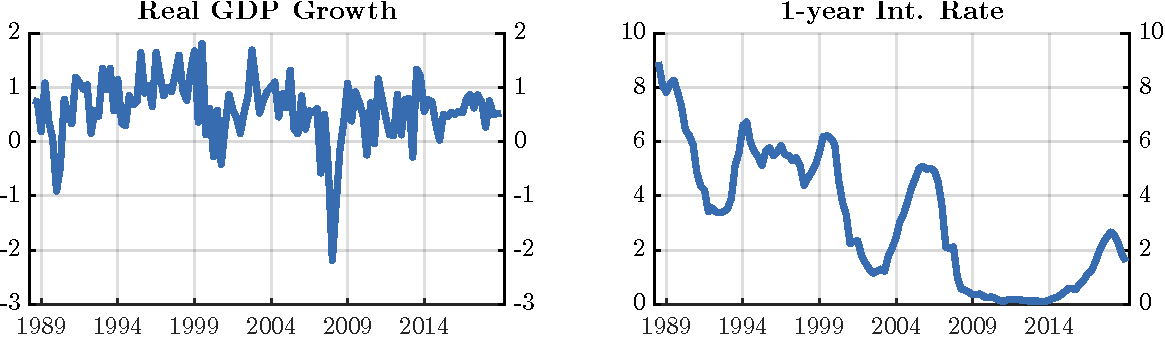
\includegraphics[width=.9\textwidth]{data}
		\end{center}%
		\vspace{0.2cm}
		\caption{\scshape{Endogenous Variables in the Simple VAR}}
		\vspace{0.2cm}
		\scriptsize{{\scshape Note.} Log-difference of US real GDP and the 1-year Treasury bill yield, the two endogenous variables of the bivariate VAR used throughout the identification examples in this handbook. Both series are in percent. Sample: 1989:Q2--2019:Q4.}
		\label{fig:data}
	\end{minipage}
\end{figure}

\subsection{Estimation}\label{sec:reducedform}

With the data in hand, we estimate the bivariate VAR(1) introduced in Section~\ref{sec:rfvar}.\footnote{Estimation hats are suppressed throughout for readability.} For reference, the model (equations \eqref{eq:red_var_1}--\eqref{eq:red_cov_1}) is:%
\begin{equation*}
	\begin{array}{c}
		y_{t}=c_y+ \phi _{11}y_{t-1}+\phi _{12}r_{t-1}+u_{yt}, \\
		r_{t}=c_r+ \phi _{21}y_{t-1}+\phi _{22}r_{t-1}+u_{rt},%
	\end{array}
\end{equation*}
which in matrix form can be written more compactly as
\begin{equation*}
	x_{t}= c + \Phi x_{t-1}+u_{t},
\end{equation*}
where $x_{t}$ is a $2 \times 1$ column vector collecting the two endogenous variables at time $t$;\footnote{The relationship between \mci{X} and $x_t$ is described in the footnote attached to equation~\eqref{eq:convention} above.} $c$ is a $2 \times 1$ vector of constants; $\Phi$ is a $2 \times 2$ matrix of autoregressive coefficients; and $u_{t}$ is a $2 \times 1$ vector of serially uncorrelated innovations, generally referred to as \textit{reduced-form residuals}.\footnote{The assumption that $u_t$ is serially uncorrelated can be tested using standard portmanteau tests (e.g.\ the Ljung-Box test) applied to the estimated residuals. Residual serial correlation typically signals that the lag order $p$ is too low or that the model is otherwise misspecified; in practice, it is good practice to increase $p$ until residual autocorrelation is no longer present.} Typically, the reduced-form residuals are correlated among themselves. Their covariance matrix can be written as:
\begin{equation*}
	\mathbb{V}(u_{t})\equiv \Sigma_{u}=\left[
	\begin{array}{cc}
		\sigma _{y}^{2} & \sigma _{yr} \\
		\sigma _{yr} & \sigma _{r}^{2}%
	\end{array}%
	\right].
\end{equation*}%
The covariance matrix $\Sigma_{u}$ is a $2 \times 2$ symmetric matrix. Its diagonal elements are the variances of the estimated reduced-form innovations, $\sigma _{y}^{2}$ and $\sigma _{r}^{2}$; and its off-diagonal elements --- equal to each other by symmetry --- give the covariance between the reduced-form residuals, $\sigma _{yr}$.

A VAR model is estimated with a single call to the function \mc{VARmodel.m}. There are three required inputs to this function: (i) a matrix of endogenous variables, \mc{X}; (ii) an integer specifying the number of lags, \mc{nlag}; and (iii) an integer specifying the deterministic component, \mc{detc} (0 = no deterministic component, 1 = constant, 2 = constant and trend). An optional fourth argument \mc{VARopt} holds all estimation and identification options (created with \mc{VARoption}; a sensible default is used if omitted). Optional fifth and sixth arguments \mc{EXOG} and \mc{nlag\_ex} accept a matrix of exogenous regressors and their lag order, respectively.

Although \mc{VARopt} is optional --- the reduced-form OLS fit can be obtained directly with \mc{VARmodel(X,nlags,detc)} --- in the example below it is created so that the variable mnemonics can be passed to \mc{VARmodel} through \mc{VARopt.mnem}. These mnemonics are used to label the estimation output, as detailed below. The code estimates the simple VAR model in \eqref{eq:red_var_1}:

\begin{matlabcode}
% Initialise VAR options and set the variable mnemonics
VARopt = VARoption;
VARopt.mnem = Xmnem;
% Deterministic component: 1=constant, 2=constant+trend
detc = 1;
% Lag order
nlags = 1;
% Estimate VAR by OLS (reduced form only)
VAR_redform = VARmodel(X,nlags,detc,VARopt);
\end{matlabcode}

\begin{notebox}
\boxentry{Choosing the lag order}
\textbf{Choosing the lag order.} \ The lag order $p$ is a critical specification choice. Setting $p$ too low leads to omitted-variable bias and serially correlated residuals; setting $p$ too high wastes degrees of freedom and inflates parameter uncertainty. Several \textit{information criteria} are available to select the VAR lag order. The two most common are:
\begin{align*}
\text{AIC} &= \ln|\hat{\Sigma}_u| + \frac{2}{T}pk^2, \\
\text{BIC} &= \ln|\hat{\Sigma}_u| + \frac{\ln T}{T}pk^2,
\end{align*}
where $k$ is the number of endogenous variables, $T$ is the sample size, and $|\hat{\Sigma}_u|$ is the determinant of the estimated residual covariance matrix. Here $pk^2$ counts the autoregressive coefficients only. In practice, \mci{VARlag} uses the total number of regressors per equation (including deterministic terms) in the penalty, replacing $pk^2$ with $k(pk+d)$ where $d$ is the number of deterministic regressors ($d=1$ for a constant, $d=2$ for a constant and trend). BIC (also known as the Schwarz Information Criterion, SIC; both acronyms refer to the same criterion) applies a heavier penalty than AIC and tends to select more parsimonious models. A \textit{sequential likelihood-ratio (LR) test} provides an alternative: start from a maximum lag $p_{\max}$ and test down, removing one lag at a time until the LR statistic first becomes insignificant.

In practice, quarterly VARs often use 4--8 lags; monthly VARs typically use 12--24. With $k$ variables and $p$ lags, each equation has $kp + d$ regressors. As a rough guideline, the total number of estimated parameters per equation should remain well below $T/10$ to preserve adequate degrees of freedom. Regardless of the criterion used, it is good practice to verify that the chosen lag order yields serially uncorrelated residuals --- a necessary condition for valid inference.

The VAR Toolbox provides the function \mci{VARlag.m} to automate lag selection. It evaluates AIC and BIC over all lag lengths from 1 to a user-specified maximum and returns the optimal lag under each criterion:
\begin{matlabcode}
[AIC, BIC, logL] = VARlag(X, maxlag, detc);
\end{matlabcode}
\noindent where \mci{X} is the matrix of endogenous variables, \mci{maxlag} is the maximum lag length to consider, and \mci{detc} is the deterministic specification (same as in \mci{VARmodel}). The function returns the optimal lag length under AIC (\mci{AIC}) and BIC (\mci{BIC}), and the log-likelihood value at each candidate lag order from 1 to \mci{maxlag} (\mci{logL}, a vector of length \mci{maxlag}). In case of disagreement between AIC and BIC, it is advisable to check robustness of the results under both.
\end{notebox}

The results of the VAR estimation are stored in the structure \mc{VAR\_redform}. Together with the options structure \mc{VARopt}, it forms one of the two central objects of the VAR Toolbox. The two play complementary roles: \mc{VARopt} is the input side --- a MATLAB struct, created once with \mc{VARoption}, that can be reused and modified across successive calls to \mc{VARmodel} and related functions, so that options set in one step carry over to the next without re-specification --- while \mc{VAR\_redform} is the output side, collecting both the inputs and the estimation results.

Specifically, \mc{VAR\_redform} stores the inputs to \mc{VARmodel.m} --- the matrix of endogenous variables (\mc{VAR\_redform.ENDO}), the chosen number of lags (\mc{VAR\_redform.nlag}), the number of endogenous variables (\mc{VAR\_redform.nvar}), and so on --- alongside the estimation output. Its fields can be inspected with \mc{disp(VAR\_redform)}, or, in the MATLAB desktop environment, by double-clicking on the structure in the Workspace browser:

\begin{matlaboutput}
>> disp(VAR_redform)
	ENDO: [123×2 double]
	nlag: 1
	const: 1
	EXOG: []
	nvar: 2
	nvar_ex: 0
	nlag_ex: 0
	ncoeff_es: 0
	nobs: 122
	ncoeff: 2
	ntotcoeff: 3
	eqnames: {2×1 cell}
	dlngdp: [1×1 struct]
	i1yr: [1×1 struct]
	Ft: [3×2 double]
	F: [2×3 double]
	sigma: [2×2 double]
	resid: [122×2 double]
	X: [122×3 double]
	Y: [122×2 double]
	Fcomp: [2×2 double]
	maxEig: 0.9559
	B: []
	PSI: []
	Fp: []
	IR: []
	VD: []
	HD: []
	ident: ''
\end{matlaboutput}

\noindent A few of the elements of the structure \mc{VAR\_redform}\ are worth describing in detail.

\begin{itemize}
\item \underline{\textit{Estimated coefficients}}. \ The matrix \mc{VAR\_redform.F} collects all estimated coefficients following the notation in \eqref{eq:red_var_1}, so that \mc{VAR\_redform.F}$=[c \ \hat{\Phi}_1 \ \cdots \ \hat{\Phi}_p]$. For the VAR(1) considered here ($p=1$, $k=2$, plus a constant), \mc{VAR\_redform.F} is a $2\times 3$ matrix, as shown below:
\begin{matlaboutput}
>> disp(VAR_redform.F)
	 0.3630    0.3788    0.0041
	-0.0729    0.2607    0.9541
\end{matlaboutput}

\item \underline{\textit{VAR residuals}} \ The matrix \mc{VAR\_redform.resid} collects the VAR reduced-form residuals, as defined by \eqref{eq:red_var_1}. The $t$-th row of \mc{VAR\_redform.resid} is the row vector $u_t'$, for $t=p+1,\ldots,T$. For a VAR with $p$ lags, \mc{VAR\_redform.resid} is a $(T-p)\times k$ matrix (as $p$ observations are lost when computing lags of $x_t$), here $122\times 2$.\medskip

\item \underline{\textit{Reduced-form covariance matrix}} \ The matrix \mc{VAR\_redform.sigma} collects the covariance matrix of the VAR reduced-form residuals defined by \eqref{eq:red_cov_1}. The convention is such that \mc{VAR\_redform.sigma}=$\Sigma_{u}$. The estimate is degrees-of-freedom corrected: $\hat{\Sigma}_u = \hat{u}'\hat{u}\,/\,(T_{\text{eff}} - (pk+d))$, where $T_{\text{eff}}=T-p$ is the number of observations left after lag removal and $pk+d$ is the number of regressors per equation --- $k$ coefficients on each of the $p$ lags, plus $d$ deterministic terms ($d=1$ for a constant, $d=2$ for a constant and trend), and any exogenous regressors when present. This count is what the toolbox stores in \mc{VAR\_redform.ntotcoeff}, equal to $3$ in the printout above ($p=1$, $k=2$, $d=1$). For a VAR with $2$ endogenous variables, the covariance matrix \mc{VAR\_redform.sigma} is a symmetric $2\times 2$ matrix:
\begin{matlaboutput}
>> disp(VAR_redform.sigma)
	0.2891    0.0782
	0.0782    0.1473
\end{matlaboutput}

\item \phantomsection\label{item:companion}\underline{\textit{Companion matrix}} \ The matrix \mc{VAR\_redform.Fcomp} stores the companion matrix. The companion matrix allows rewriting VARs with lags greater than $1$ as VAR(1) (see Box~\ref{box:companion} in Section~\ref{sec:stability}). For a VAR(1), the companion matrix \mc{VAR\_redform.Fcomp} equals \mc{VAR\_redform.F} with the deterministic columns removed. The companion matrix plays a central role in computing impulse responses and in implementing identification schemes; Section~\ref{sec:dynamic} develops this in detail (see also Box~\ref{box:companion} in Section~\ref{sec:stability}).\medskip

\item \underline{\textit{Equation-by-equation estimation output}}. The structures \mc{VAR\_redform.dlngdp} and \mc{VAR\_redform.i1yr} include the OLS equation-by-equation estimation results (coefficients, standard errors, $t$-statistics, $p$-values, fitted values, residuals, and goodness-of-fit statistics for each equation). These sub-structures take their names from the mnemonics in \mc{VARopt.mnem}, set above to \mc{\{'dlngdp','i1yr'\}}, so each equation is accessed by variable name --- convenient for reading the output of larger systems. When \mc{mnem} is not provided the sub-structures are named \mc{eq1}, \ldots, \mc{eqk} instead; the same fallback applies whenever \mc{mnem} is empty, of the wrong length, non-unique, contains entries that are not valid field names (e.g.\ labels with spaces), or clashes with a reserved field of the VAR structure. The resolved names are also recorded in \mc{VAR\_redform.eqnames}, a $k\times 1$ cell array (here \mc{\{'dlngdp','i1yr'\}}) that downstream functions such as \mc{VARprint} use to read the equations by the same labels. The labelling affects only the field names: the contents and the column order of every output are unchanged. The mnemonics in \mc{VARopt.mnem} are used solely to name these sub-structures, while \mc{VARopt.vnames} holds the variable labels used by the plotting functions.
\end{itemize}

\noindent The VAR structure includes several empty objects, which fall into two categories. Some are empty because they depend on an identification step that has not yet been performed. The most important is \mc{VAR\_redform.B}, which stores the \textit{structural impact matrix} $B$ --- the $k\times k$ matrix defined by $u_t = B\varepsilon_t$ (equation \eqref{eq:struct_shocks}) that links structural shocks to reduced-form residuals. Since identification is taken up in Section~\ref{sec:ident}, \mc{VAR\_redform.B} remains empty for now. Others are empty because the current specification does not include the corresponding feature. For example, \mc{VAR\_redform.EXOG} stores any variables treated as fully exogenous: variables entered as additional regressors in every equation of the VAR but not modeled as endogenous. In the current bivariate VAR no exogenous variables are included (\mc{nvar\_ex = 0}), so \mc{VAR\_redform.EXOG} is empty. A natural application where one would populate \mc{VAR\_redform.EXOG} is, for example, a small open economy VAR, where world oil prices are typically treated as fully exogenous on the grounds that the small economy cannot affect them. Rather than adding oil prices as an endogenous variable --- which would require modeling their dynamics as a function of the domestic variables --- they enter each equation as exogenous regressors, passed as the optional fifth argument of \mc{VARmodel} (after \mc{VARopt}), with a user-specific number of lags.

The structure \mc{VARopt} is created by \mc{VARoption} and holds all options for identification, inference, and plotting. Table~\ref{tab:varopt} lists every field, grouped by role, together with its default value and meaning; the table mirrors the content in \mc{VARoption.m}, which can be inspected directly for the same information. All fields have sensible defaults; the user sets only those relevant to the current step.\bigskip

\begingroup
\footnotesize
\setlength{\defaultaddspace}{0.8em}
\renewcommand{\arraystretch}{0.9}
\renewcommand{\mc}[1]{\colorbox{script!80}{\texttt{#1}}}
\begin{longtable}{l@{\hspace{0.7em}}p{0.6\textwidth}}
\caption{Fields of the \mc{VARopt} options structure, with default values.}\label{tab:varopt}\\\toprule
\textbf{Field (default)} & \textbf{Description}\\
\midrule
\endfirsthead
\multicolumn{2}{l}{\itshape Table~\ref{tab:varopt}, continued}\\
\toprule
\textbf{Field (default)} & \textbf{Description}\\
\midrule
\endhead
\midrule
\multicolumn{2}{r}{\footnotesize\itshape continued on next page}\\
\endfoot
\bottomrule
\endlastfoot
\addlinespace
\multicolumn{2}{l}{\underline{\textit{Variable and shock labels}}}\\[2pt]
\mc{mnem = []}            & Endogenous variable mnemonics: valid MATLAB identifiers (no spaces or special characters) used to name the per-equation sub-structs. Falls back to \mc{eq1},\ldots,\mc{eqN} if empty or invalid.\\
\mc{vnames = []}          & Endogenous variable names: display labels for plots and tables (may contain spaces or \LaTeX). Falls back to \mc{mnem} if empty.\\
\mc{vnames\_ex = []}      & Exogenous variable names.\\
\mc{snames = []}          & Shock names (default to \mc{vnames} if empty).\\
\addlinespace
\multicolumn{2}{l}{\underline{\textit{Identification}}}\\[2pt]
\mc{ident = ''}           & Identification scheme: \mc{''} (none, reduced form only), \mc{'short'} (zero contemporaneous), \mc{'long'} (zero long-run), \mc{'sign'} (sign restrictions), \mc{'sign+iv'} (sign restrictions with an IV-identified first shock), \mc{'iv'} (external instrument), \mc{'exog'} (exogenous variable).\\
\mc{IV = []}              & External instrument matrix for \mc{ident='iv'} or \mc{'sign+iv'}.\\
\mc{exoshock = []}        & Exogenous shock variable for \mc{ident='exog'}.\\
\mc{nlag\_exoshock = 0}   & Lag order for \mc{exoshock} (0 = contemporaneous only).\\
\addlinespace
\multicolumn{2}{l}{\underline{\textit{IRF and FEVD computation}}}\\[2pt]
\mc{nsteps = 40}          & Number of horizons for IRFs and FEVDs.\\
\mc{impact = 0}           & Shock size: 0 = one standard deviation, 1 = unit shock.\\
\mc{shut = 0}             & Force the IRF of one variable to zero (0 = off).\\
\mc{recurs = 'wold'}      & MA representation: \mc{'wold'} (recursive Wold) or companion form \mc{'comp'}.\\
\addlinespace
\multicolumn{2}{l}{\underline{\textit{Inference}}}\\[2pt]
\mc{inference = 1}        & 1 = parameter uncertainty (default); 0 = point estimates only.\\
\mc{ndraws = 1000}        & Number of bootstrap draws.\\
\mc{mult = 10}            & Print progress every \mc{mult} draws.\\
\mc{pctg = 95}            & Outer confidence level for error bands (percent).\\
\mc{method = 'bs'}        & Bootstrap method: \mc{'bs'} standard, \mc{'wild'} wild.\\
\addlinespace
\multicolumn{2}{l}{\underline{\textit{Sign restrictions}}}\\[2pt]
\mc{R = []}               & Sign restriction matrix or struct (required for \mc{ident='sign'} or \mc{'sign+iv'}).\\
\mc{sr\_hor = 1}          & Number of periods over which sign restrictions apply.\\
\mc{sr\_rot = 500}        & Maximum rotations per draw.\\
\mc{sr\_draw = 100000}    & Maximum total draws.\\
\addlinespace
\multicolumn{2}{l}{\underline{\textit{Figure export}}}\\[2pt]
\mc{pick = 0}             & Shock to plot: 0 = all, \mc{j} = shock \mc{j} only.\\
\mc{quality = 2}          & Export quality: 2 = high via \mc{exportgraphics} (recommended, R2020a+), 1 = high via Ghostscript (legacy fallback), 0 = low via \mc{print -dpdf}.\\
\mc{suptitle = 0}         & 1 = add a super-title above the figure panels.\\
\mc{firstdate = []}       & First sample date (e.g.\ \mc{1999.75} = 1999Q4); with \mc{frequency}, controls the axis date labels.\\
\mc{frequency = 'q'}      & Data frequency: \mc{'q'} quarterly, \mc{'m'} monthly, \mc{'y'} yearly.\\
\mc{datenticks = 5}       & Target number of date ticks on the x-axis (HD plots); fewer avoids slanted year labels in narrow panels.\\
\mc{figname = []}         & Prefix string for the exported figure filename.\\
\mc{figsize = []}         & Figure window size \mc{[width, height]} in cm.\\
\addlinespace
\multicolumn{2}{l}{\underline{\textit{Panel appearance (used by all plot functions)}}}\\[2pt]
\mc{latex = 1}            & 1 = use the \LaTeX{} interpreter for figure text.\\
\mc{font = 'Helvetica'}   & Font name for figure text; \mc{''} = MATLAB default.\\
\mc{grid = 1}             & 1 = show gridlines.\\
\mc{marker = 'o'}         & Marker style for the IRF line (\mc{'o'}, \mc{'none'}, etc.).\\
\mc{subplot = []}         & Subplot grid \mc{[rows cols]}; empty = auto from \mc{sqrt(nvars)}.\\
\mc{shorttitle = 0}       & 1 = show the variable name only as the panel title.\\
\mc{color = []}           & Line and band color (RGB triplet); empty = \mc{pantone('Blue')}.\\
\mc{linestyle = '-'}      & IRF line style (\mc{'-'}, \mc{'--'}, \mc{':'}, \mc{'-.'}).\\
\mc{hstart = 1}           & First horizon label on the x-axis (0 or 1).\\
\mc{xlim = []}            & x-axis limits \mc{[lo hi]}; empty = auto.\\
\mc{ylim = []}            & y-axis limits \mc{[lo hi]}; empty = auto.\\
\mc{xtick = []}           & x-tick positions; empty = auto.\\
\mc{xlabel = ''}          & x-axis label applied to each panel; empty = none.\\
\mc{ylabel = ''}          & y-axis label applied to each panel; empty = none.\\
\mc{dualaxis = 1}         & 1 = dual-axis panel style (tick marks mirrored on the left and right y-axes, box off, closure tick at the top); 0 = off.\\
\mc{visible = 1}          & 1 = show figure windows; 0 = suppress display (save only).\\
\mc{legcols = 1}          & Number of columns in the legend.\\
\mc{legloc = 'best'}      & Legend location: \mc{'best'} = auto-corner, or any explicit MATLAB location string.\\
\addlinespace
\multicolumn{2}{l}{\underline{\textit{Historical decomposition plot (\mc{VARhdplot})}}}\\[2pt]
\mc{hd\_colors = []}      & RGB matrix (\mc{ncols}$\times$3) overriding bar colors in stack order; empty = use the default colormap.\\
\mc{hd\_detc = 1}         & 1 = stack all HD components (const, trend, init, exogenous, shocks), with bars summing to the \mc{Data} line; 0 = stack shock contributions only, with the reference line equal to data minus const and init.\\
\addlinespace
\multicolumn{2}{l}{\underline{\textit{Narrative restrictions}}}\\[2pt]
\mc{dates = []}           & Cell array of date strings, one per observation; required by \mc{SR.m} for string-format narrative periods.\\
\end{longtable}
\endgroup

\noindent The most important fields are the identification scheme (\mc{ident}), the external instrument (\mc{IV}), the sign restriction matrix or struct (\mc{R}), the number of IRF horizons (\mc{nsteps}), the mnemonics that name the equation sub-structs (\mc{mnem}), the variable labels used by the plotting functions (\mc{vnames}), the confidence level for bootstrap bands (\mc{pctg}), and the flag for inference for impulse responses, variance decompositions, and historical decompositions (\mc{inference}). Because the default is \mc{inference = 1}, the structural examples in Section~\ref{sec:ident} will set \mc{inference = 0} explicitly so that the figures report point estimates; statistical inference is introduced separately in Section~\ref{sec:inference}. For example, the code below adds variable labels before printing the OLS table:

\begin{matlabcode}
% Add display labels to VARopt before printing the coefficient table
VARopt.vnames = Xvnames;
\end{matlabcode}

\noindent Finally, the VAR Toolbox provides a built-in function to display the most important estimation results in the command window:

\begin{matlabcode}
% Print OLS coefficient table and return the raw beta matrix
[TABLE, beta] = VARprint(VAR_redform,VARopt);
\end{matlabcode}

\noindent which produces the following output in the MATLAB command window:

\begin{matlaboutput}
Reduced-form VAR estimation:

                         Real GDP Growth    1-year Int. Rate 
constant                       0.3630          -0.0729 
Real GDP Growth(-1)            0.3788           0.2607 
1-year Int. Rate(-1)           0.0041           0.9541 

VAR eigenvalues:
0.3769
0.95592

Reduced-form covariance matrix:
0.28909       0.078151
0.078151      0.14726
\end{matlaboutput}

\noindent The columns of the printed table correspond to the equations of the VAR (one per endogenous variable), and the rows list the constant $c$ and the elements of the lag coefficient matrices $\Phi_1, \ldots, \Phi_p$ in equation~\eqref{eq:red_var_1}: a row labelled \mc{VariableName(-j)} gives the coefficient on the $j$-period lag of that variable in each equation. The cell array \mc{beta} includes the estimated values of the coefficients in the VAR, while the cell array \mc{TABLE} includes --- in addition to the estimated coefficients --- their standard errors, t-statistics, and p-values.

\noindent \textbf{\sffamily\underline{Checking stability}.} The VAR Toolbox automatically computes the eigenvalues of the companion matrix $\mathcal{F}$ during estimation, as discussed in Section~\ref{sec:stability}. The maximum eigenvalue (in modulus) is stored in \mc{VAR\_redform.maxEig}:

\begin{matlaboutput}
>> disp(VAR_redform.maxEig)
	0.9559
\end{matlaboutput}
A maximum modulus strictly less than one confirms that all eigenvalues of $\mathcal{F}$ lie inside the unit circle and the VAR is stable. All eigenvalues of the companion matrix \mc{VAR\_redform.Fcomp} can be inspected via MATLAB's \mc{eig} function:\footnote{Note that \mci{VAR\_redform.Fcomp} is the companion matrix built excluding the constant $c$ from the coefficient matrix \mci{VAR\_redform.F}. See Box~\ref{box:companion} for more details on how to construct the companion matrix.}

\begin{matlaboutput}
>> disp(eig(VAR_redform.Fcomp))
	0.3769
	0.9559
\end{matlaboutput}
If any eigenvalue exceeds one in modulus, the VAR is unstable and the impulse responses, variance decompositions, and other dynamic analyses discussed in Section~\ref{sec:dynamic} will not be well-defined. Common remedies include adjusting the lag order, re-examining the variable selection, or transforming non-stationary variables (e.g.\ by first-differencing).

\noindent \textbf{\sffamily\underline{In sum.}} \ This section has shown how to estimate the reduced-form VAR by OLS, delivering $\hat{c}$, $\hat{\Phi}_1,\ldots,\hat{\Phi}_p$, $\hat{\Sigma}_u$, and the eigenvalues of the companion matrix. These objects fully characterize the linear dynamics of $x_t$ but carry no structural interpretation. Recovering economically meaningful shocks requires solving the identification problem introduced in Section~\ref{sec:identproblem}: finding a $k\times k$ matrix $B$ such that $\Sigma_u = BB'$. As established there, this system is underdetermined --- in the bivariate case, the three independent equations from $\Sigma_u = BB'$ cannot pin down all four elements of $B$. This is reflected directly in the \mc{VAR\_redform} structure: after estimation, \mc{VAR\_redform.B} is empty (as seen in the output above), because the link between reduced-form residuals and structural shocks has not yet been established. Section~\ref{sec:ident} addresses this challenge by imposing economic restrictions that select a unique $B$ matrix.

\section{Identification in the VAR Toolbox}\label{sec:ident}

The identification problem described in the previous section admits several solutions. This section describes how to implement some of the most popular ones through simple examples using the VAR Toolbox. As noted in Section~\ref{sec:rfvar_toolbox}, the examples throughout this section are run with parameter uncertainty switched off (\mc{VARopt.inference = 0}), so that the figures display point estimates and the discussion can focus on identification alone; although \mc{VARopt.inference = 1} is the toolbox default, it is disabled here and taken up in detail in Section~\ref{sec:inference}. Specifically, the next subsections cover the following identification schemes: zero contemporaneous restrictions, zero long-run restrictions, sign restrictions, narrative sign restrictions, external instruments, combined sign-IV restrictions, and exogenous variables.

\subsection{Zero Contemporaneous Restrictions}\label{sec:short}

Identification using zero contemporaneous restrictions --- also known as Cholesky or recursive identification (see the notebox below for why this label is imprecise) --- was developed by \cite{Sims1980}, and has long been one of the most widely used identification schemes in the literature. The underlying idea is that some structural shocks may take time to transmit through the economy, and therefore have no contemporaneous effects on one or more of the endogenous variables in the VAR. For example, it is widely believed that there are substantial lags in the transmission of monetary policy to the real economy. Under this assumption, one could impose that monetary policy shocks have zero contemporaneous effects on one (or a subset) of the endogenous variables in the VAR. 

The bivariate VAR makes this intuition precise. As established in Section~\ref{sec:struct_var}, the VAR is underidentified: the three independent equations from $\Sigma_u = BB'$ leave one element of $B$ unconstrained. Imposing zero contemporaneous restrictions amounts to assuming that some of the non-diagonal elements of $B$ are equal to zero, thus reducing the number of unknown coefficients. 

In the simple case considered here, it will therefore suffice to set to zero one element of the $B$ matrix to solve for the remaining three elements with the three available equations. The question is which element of the $B$ matrix to set to zero. One could maintain the assumption that a monetary policy shock affects the short-term interest rate on impact (i.e.\ $r_{t}$) but takes time to transmit to the real economy, and affect output ($y_{t}$) only with a lag. This identifying assumption implies that $b_{12}=0$, so that the structural VAR can be written as:
\begin{equation}
	\left[
	\begin{array}{c}
		y_{t} \\
		r_{t}%
	\end{array}%
	\right] =%
	\begin{bmatrix}
		c_{y} \\
		c_{r} %
	\end{bmatrix}
	+
	\begin{bmatrix}
		\phi _{11} & \phi _{12} \\
		\phi _{21} & \phi _{22}%
	\end{bmatrix}%
	\left[
	\begin{array}{c}
		y_{t-1} \\
		r_{t-1}%
	\end{array}%
	\right] +\left[
	\begin{array}{cc}
		b_{11} & 0 \\
		b_{21} & b_{22}%
	\end{array}%
	\right]
	\begin{bmatrix}
		\varepsilon_{t}^{Demand} \\
		\varepsilon_{t}^{MonPol}%
	\end{bmatrix}%
	,  \label{eq:struct_var_ch}
\end{equation}
so that $y_{t}$ is not contemporaneously affected by $\varepsilon_{t}^{MonPol}$, while $r_{t}$ is contemporaneously affected by both $\varepsilon_{t}^{Demand}$ and $\varepsilon_{t}^{MonPol}$, through the coefficients $b_{21}$ and $b_{22}$. As we now have $3$ independent equations and $3$ unknowns, we can recover the elements of the $B$ matrix by solving the system of equations implied by $\Sigma_u=BB'$. The structural VAR is thus identified.

\noindent \textbf{\sffamily\underline{Math}.} Zero short-run restrictions achieve identification by reducing the number of free parameters in $B$ until it matches the number of independent equations supplied by $\Sigma_u = BB'$. The number of restrictions required depends on the size of the VAR: for a VAR with $k$ endogenous variables, exact identification requires $k(k-1)/2$ zero restrictions --- a count that grows quadratically in $k$. In the bivariate case, a single restriction ($b_{12}=0$) suffices, as established above. The explicit solution follows from expanding $\Sigma_u = BB'$:
\begin{equation}\label{eqapp:short1}
	\left[
	\begin{array}{cc}
		\sigma _{y}^{2} & \sigma _{yr} \\
		- & \sigma _{r}^{2}%
	\end{array}%
	\right] =\underset{B}{\underbrace{\left[
			\begin{array}{cc}
				b_{11} & b_{12} \\
				b_{21} & b_{22}%
			\end{array}%
			\right] }}\underset{B'}{\underbrace{\left[
			\begin{array}{cc}
				b_{11} & b_{21} \\
				b_{12} & b_{22}%
			\end{array}%
			\right] }}
		\Rightarrow
		\left\{
		\begin{array}{l}
			\sigma _{y}^{2}=b_{11}^{2}+b_{12}^{2} \\
			\sigma _{yr}=b_{11}b_{21}+b_{12}b_{22} \\
			\sigma _{yr}=b_{11}b_{21}+b_{12}b_{22} \\
			\sigma _{r}^{2}=b_{21}^{2}+b_{22}^{2}%
		\end{array}%
		\right. 
\end{equation}%
The middle two equations are identical, leaving three independent equations in four unknowns. Setting $b_{12}=0$ reduces it to:%
\begin{equation}\label{eqapp:short2}
	\left\{
	\begin{array}{l}
		\sigma _{y}^{2}=b_{11}^{2}, \\
		\sigma _{yr}=b_{11}b_{21}, \\
		\sigma _{r}^{2}=b_{21}^{2}+b_{22}^{2}.%
	\end{array}%
	\right.
\end{equation}%
which can be solved to yield:
\begin{equation}\label{eqapp:short3}
	\left\{
	\begin{array}{l}
		b_{11}=\sigma _{y}, \\
		b_{21}=\sigma _{yr}/\sigma _{y}, \\
		b_{22}=\sqrt{\sigma _{r}^{2}-\frac{\sigma _{yr}^{2}}{\sigma _{y}^{2}}}.%
	\end{array}%
	\right.
\end{equation}%
which shows that the VAR is identified. The same solution can be obtained directly via the Cholesky decomposition of $\Sigma_u$. Denote by $P$ the unique lower-triangular Cholesky factor of $\Sigma_u$, so that $\Sigma_u = PP'$. Because $P$ is unique, it follows that $B=P$ (see notebox below for details).

\begin{notebox}
\boxentry{The Cholesky decomposition}
\textbf{The Cholesky decomposition.} \ The identification by zero short-run restrictions is often referred to as `Cholesky' identification. The reason is that the solution above can be obtained with a Cholesky decomposition of the reduced-form covariance matrix. The label is nonetheless imprecise: the Cholesky factorization is a general-purpose tool that applies to any symmetric positive-definite matrix, and is used in other identification schemes as well --- including identification by long-run restrictions (Section~\ref{sec:long}). What is specific to the present approach is not the factorization method but the economic assumption it encodes: that some structural shocks have no contemporaneous effect on some endogenous variables.

\indent Specifically, a symmetric and positive-definite matrix like $\Sigma_{u}$ always admits the following unique decomposition:
\begin{equation}\label{eqapp:short4}
	\Sigma_{u}=\left[
	\begin{array}{cc}
		\sigma _{y}^{2} & \sigma _{yr} \\
		\sigma _{yr} & \sigma _{r}^{2}%
	\end{array}%
	\right] =\left[
	\begin{array}{cc}
		p_{11} & 0 \\
		p_{21} & p_{22}%
	\end{array}%
	\right] \left[
	\begin{array}{cc}
		p_{11} & p_{21} \\
		0 & p_{22}%
	\end{array}%
	\right] =PP'
\end{equation}%
where the lower-triangular matrix $P$ is known as the Cholesky factor of $\Sigma_{u}$. Recalling that (i) $\Sigma_{u}=BB'$ and (ii) $B$ is lower triangular by assumption ($b_{12}=0$), and noting that the Cholesky factorization of a positive-definite matrix is unique, it follows that $P=B$. This is particularly useful for large VARs, since the system of equations implied by $\Sigma_u = BB'$ becomes increasingly complex as the dimensionality of the VAR increases. Instead of solving by hand the system of equations \eqref{eqapp:short2}, the Cholesky factor of $\Sigma_u$ can be computed in MATLAB as follows:

\begin{matlaboutput}
>> chol(VAR.sigma,'lower')
ans= 
	0.5377         0
	0.1454    0.3552
\end{matlaboutput}

\noindent which equals the solution to \eqref{eqapp:short3}, as can be verified by substitution.
\end{notebox}

\noindent \textbf{\sffamily\underline{In MATLAB}.} Zero short-run restrictions can be implemented in the VAR Toolbox with a few lines of code. The structure \mc{VARopt} includes a field that allows the user to choose what identification scheme to employ. The mnemonic for the identification by short-run restrictions is the string \mc{'short'}. So, zero contemporaneous (or short-run) restrictions can be selected by executing the following line of code:

\begin{matlabcode}
% Select zero short-run identification
VARopt.ident = 'short';
\end{matlabcode}

%claude
\noindent It is also useful (but not necessary) to update the \mc{VARopt} structure with a few additional details. As discussed above, \mc{VARopt.inference} is set to zero so as to focus on point estimates only. The remaining options are useful for the output, e.g.\ for equation names for plotting and saving impulse responses:

\begin{matlabcode}
% Additional options
VARopt.inference = 0;                    % Point estimates only
VARopt.mnem   = Xmnem;                   % mnemonics name the VAR.(.) sub-structs
VARopt.vnames = Xvnames;                 % variable names in plots
VARopt.nsteps = 20;                      % max horizon of IRF
VARopt.figsize = [24,6];                 % size of window (figures)
VARopt.firstdate = datesnum(1);          % first date in plots
VARopt.frequency = 'q';                  % frequency of the data
VARopt.snames = {bfeps('Demand'), bfeps('MonPol')}; % shock names
VARopt.figname = 'graphics/short';
\end{matlabcode}

\noindent Once \mc{VARopt.ident} is set, a single call to \mc{VARmodel} performs identification and computes impulse responses (as well as other structural objects such as variance and historical decompositions, which will be discussed in more detail in Section~\ref{sec:dynamic}):

\begin{matlabcode}
% Compute impulse responses and plot the MP shock (pick=2)
VAR_short = VARmodel(X,nlags,detc,VARopt);
\end{matlabcode}

\noindent The \mc{VARmodel} call returns a structure \mc{VAR\_short} that now contains, in addition to the OLS estimates from Section~\ref{sec:reducedform}, the identified structural impact matrix \mc{VAR\_short.B} and the impulse responses \mc{VAR\_short.IR}. The $B$ matrix can be printed at screen by executing the following command:

\begin{matlaboutput}
>> disp(VAR_short.B)
	0.5377         0
	0.1454    0.3552
\end{matlaboutput}

\noindent As discussed above in Section~\ref{sec:struct_var}, the $B$ matrix is crucial to be able to track the effects of a shock through the system. Consider a unit surprise in $\varepsilon_{t}^{MonPol}$, i.e.\ a surprise tightening in monetary policy, in the structural VAR in equation \eqref{eq:struct_var_ch}. What are the impact effects of such a shock on output growth $y_{t}$ and the short-term interest rate $r_{t}$? The answer is the second column of $B$. To see this, set $\varepsilon_t^{Demand}=0$ and $\varepsilon_t^{MonPol}=1$:\medskip
\begin{equation*}
	\left[
	\begin{array}{c}
		y_{t} \\
		r_{t}%
	\end{array}%
	\right] =%
	\left[
	\begin{array}{cc}
		b_{11} & 0 \\
		b_{21} & b_{22}%
	\end{array}%
	\right]
	\begin{bmatrix}
		\varepsilon_{t}^{Demand} \\
		\varepsilon_{t}^{MonPol}%
	\end{bmatrix} = 
	\small
	\left[
	\begin{array}{cc}
		\texttt{0.5377} & \texttt{0} \\
		\texttt{0.1454} & \texttt{0.3552}%
	\end{array}%
	\right]
	\begin{bmatrix}
		\texttt{0} \\
		\texttt{1}%
	\end{bmatrix}=
	\begin{bmatrix}
		\texttt{0} \\
		\texttt{0.3552}
	\end{bmatrix}\medskip
\end{equation*}%
The response of output is equal to $0$ --- not surprisingly, as we assumed so. The response of the interest rate is instead equal to $0.3552$. These impact effects propagate according to the companion matrix $\mathcal{F}$ (which equals $\Phi$ for the VAR(1) considered here). For example, the response at horizon $h=1$ is:\medskip
\begin{equation*}
	\left[
	\begin{array}{c}
		y_{t+1} \\
		r_{t+1}%
	\end{array}%
	\right] =%
	\left[
	\begin{array}{cc}
		\phi_{11} & \phi_{12} \\
		\phi_{21} & \phi_{22}%
	\end{array}%
	\right]
	\begin{bmatrix}
		y_{t}\\
		r_{t}%
	\end{bmatrix} = 
	\small
	\left[
	\begin{array}{cc}
		\texttt{0.3788} & \texttt{0.0041} \\
		\texttt{0.2607} & \texttt{0.9541}%
	\end{array}%
	\right]
	\begin{bmatrix}
		\texttt{0} \\
		\texttt{0.3552}%
	\end{bmatrix}=
	\begin{bmatrix}
		\texttt{0.0015} \\
		\texttt{0.3388}
	\end{bmatrix}\medskip
\end{equation*}%
To see that, execute the following command:

\begin{matlaboutput}
>> disp(VAR_short.Fcomp*VAR_short.B(:,2))
	0.0015
	0.3388
\end{matlaboutput}

\noindent This gives the impulse response at horizon $h=1$ (one quarter after the shock). The impulse response at any subsequent horizon can be computed analogously by repeatedly pre-multiplying by $\Phi$ (see Section~\ref{sec:dynamic} for additional details). 

\begin{notebox}
\boxentry{Variable ordering matters}
	\textbf{Variable ordering matters!} As explained above, zero short-run restrictions are achieved with a Cholesky decomposition of the reduced-form covariance matrix. This implies that the ordering of the variables in the matrix \mci{X} matters. The \mci{'short'} option implicitly assumes that the \mci{B} matrix is lower triangular. In turn this means that the structural shock associated with the first equation affects all variables in the system (as captured by the first column of the \mci{B} matrix); the structural shock associated with the second equation has zero contemporaneous effect on the first endogenous variable, but affects all subsequent variables in the system; etc. The variable ordering therefore encodes an economic assumption: the variable placed first is treated as causally prior to all others at the same point in time. The ordering should therefore be chosen to be consistent with economic theory and prior intuition.
\end{notebox}

The impulse responses are stored in \mc{VAR\_short.IR}, with dimension \mc{VARopt.nsteps} $\times$ $k$ $\times$ $k$ (here $20\times2\times2$, as \mc{VARopt.nsteps = 20} was set above). Because MATLAB uses 1-based indexing, \mc{IR(h+1,:,j)} stores the response at horizon $h$: \mc{IR(1,:,j)} is the impact response ($h=0$), \mc{IR(2,:,j)} is $h=1$, and so on.  The built-in function \mc{VARirplot.m} can be used to plot the impulse responses:

\begin{matlabcode}
VARopt.pick = 2;
VARirplot(VAR_short.IR,VARopt);
\end{matlabcode}

\noindent Figure~\ref{fig:short} reports the point estimates of the impulse responses of the log-difference of US real GDP and the 1-year Treasury bill yield to the monetary policy shock. On impact, the monetary policy tightening has no effect on output growth --- by construction, given the zero restriction $b_{12}=0$ --- while the interest rate rises on impact, reflecting the tightening. In subsequent periods, output rises, contrary to standard theoretical predictions. This anomalous result reflects the extreme parsimony of the bivariate VAR(1); its purpose is illustrative rather than empirical.

\vspace{0.2cm}
\begin{figure}[ht!]
	\centering%
	\begin{minipage}[b]{.9\textwidth}
		\begin{center}
			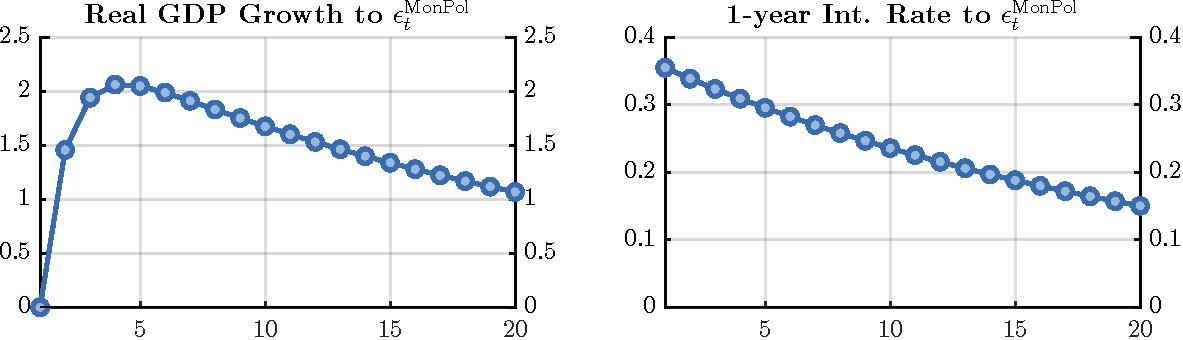
\includegraphics[width=.9\textwidth]{short}
		\end{center}%
		\vspace{0.2cm}
		\caption{\scshape{Impulse Responses to a Monetary Policy Shock:\\ Zero Contemporaneous Restrictions}}
		\vspace{0.2cm}
		\scriptsize{{\scshape Note.} Point estimates of the impulse responses of the log-difference of US real GDP and the 1-year Treasury bill yield to a contractionary monetary policy shock (tightening). Identification: zero short-run restrictions, which impose that the monetary policy shock has no contemporaneous effect on the log-difference of US real GDP ($b_{12}=0$). Bivariate VAR(1) estimated on quarterly US data, 1989:Q1--2019:Q4. Horizon: 20 quarters. Percentage points.}
		\label{fig:short}
	\end{minipage}
\end{figure}

Finally, note that a time series of structural shocks can be recovered from $\varepsilon_t = B^{-1}u_t$. Since $B$ is lower-triangular with positive diagonal entries (a consequence of the Cholesky factorization with the sign normalization), it is invertible. In MATLAB, the structural shocks can be computed by executing a single line of code:

\begin{matlabcode}
% Recover structural shocks as B^{-1} * reduced-form residuals
eps_short = (VAR_short.B\VAR_short.resid')';
\end{matlabcode}

\noindent where \mc{eps\_short} is the $T \times 2$ matrix of structural shocks. The structural shocks can be verified to be orthogonal by typing in the command window:

\begin{matlaboutput}
>> disp(corr(eps_short))
	1.0000    0.0000
	0.0000    1.0000
\end{matlaboutput}

\noindent which implies that the covariance matrix of the structural shocks is diagonal.

\subsection{Zero Long-Run Restrictions}\label{sec:long}

Zero long-run restrictions, proposed by \cite{BlanchardQuah1989}, achieve identification by the same logic as zero contemporaneous restrictions --- but impose the zeros on the long-run cumulative effects of structural shocks rather than on their contemporaneous effects. 

A well-known implication of many macroeconomic models is that supply shocks have a permanent effect on the level of output. Monetary policy shocks, by contrast, are assumed to have no long-run effect on output --- a property known as long-run monetary neutrality, which provides the identifying restriction imposed below. Under this assumption, one could impose that monetary policy shocks have no cumulative long-run effect on the level of output.

But how does one map the $B$ matrix, which captures the contemporaneous effects of structural shocks on the endogenous variables in the VAR, to the long-run effects of structural shocks? To give intuition in the context of the simple bivariate VAR described in the previous section, assume that the two shocks driving the model economy are a supply shock ($\varepsilon_t^{Supply}$) and a monetary policy shock ($\varepsilon_t^{MonPol}$):
\begin{equation}
	\left[
	\begin{array}{c}
		y_{t} \\
		r_{t}%
	\end{array}%
	\right] =%
	\begin{bmatrix}
		c_{y} \\
		c_{r} %
	\end{bmatrix}
	+
	\begin{bmatrix}
		\phi _{11} & \phi _{12} \\
		\phi _{21} & \phi _{22}%
	\end{bmatrix}%
	\left[
	\begin{array}{c}
		y_{t-1} \\
		r_{t-1}%
	\end{array}%
	\right] +\left[
	\begin{array}{cc}
		b_{11} & b_{12} \\
		b_{21} & b_{22}%
	\end{array}%
	\right]
	\begin{bmatrix}
		\varepsilon_{t}^{Supply} \\
		\varepsilon_{t}^{MonPol}%
	\end{bmatrix}%
	,  \label{eq:struct_var_bq}
\end{equation}
The effect of these structural shocks on the endogenous variables at horizon $h \geq 0$ (where $h=0$ is the period when the shock hits) can be traced by iterating the structural VAR forward. Setting all shocks after period $t$ to zero ($\varepsilon_{t+h}=0$ for all $h\geq 1$) and tracing the propagation of a single shock $\varepsilon_t$:
\begin{equation}
	\begin{array}{l}
		x_{t}=B\varepsilon_{t}, \\
		x_{t+1}=\Phi B\varepsilon_{t}, \\
		... \\
		x_{t+\infty }=\Phi ^{\infty }B\varepsilon_{t}.%
	\end{array}
	\label{eq:long1}
\end{equation}%
The long-run (i.e.\ for $h$ that goes to infinity) cumulative effect of the shock can be obtained by summing all the terms in \eqref{eq:long1}:
\begin{equation}
	x_{t,t+\infty }=B\varepsilon_{t}+\Phi B\varepsilon_{t}+\Phi
	^{2}B\varepsilon_{t}+...+\Phi ^{\infty }B\varepsilon
	_{t}=\sum\limits_{j=0}^{\infty }\Phi ^{j}B\varepsilon_{t},  \label{eq:long2}
\end{equation}%
where $x_{t,t+\infty}$ denotes the cumulative sum of the impulse response vectors in \eqref{eq:long1} from horizon $h=0$ to $\infty$. Finally, note that if the VAR is stable (i.e.\ if all eigenvalues of $\Phi$ lie strictly inside the unit circle; for the VAR(1) considered here, $\Phi = \mathcal{F}$, the companion matrix), the infinite sum in equation (\ref{eq:long2}) converges to:
\begin{equation}
	x_{t,t+\infty }=\left( I-\Phi \right) ^{-1}B\varepsilon_{t}=C\varepsilon
	_{t},  \label{eq:long3}
\end{equation}%
where
\begin{equation}\label{eq:long4}
	C\equiv \left( I-\Phi \right) ^{-1}B  
\end{equation}
is a $2 \times 2$  matrix which captures the cumulative effect of shocks $\varepsilon_{t}$ on $x_{t}$ from time $t$ to $t+\infty $.

The idea behind identification through zero long-run restrictions is to impose a zero restriction on the long-run impact matrix $C$. For example, one could maintain the assumption that monetary policy shocks have no long-run effect on the level of output. This restriction is well-defined only when the log-level of output is integrated of order one, so that the level of output has a well-defined long-run response; in the present example, $y_t$ is the log-difference of GDP, and its cumulative sum measures the log-level change. Equation (\ref{eq:long3}) allows one to impose this restriction exactly by setting $c_{12}=0$:
\begin{equation}\label{eq:long5}
	\left[
	\begin{array}{c}
		y_{t,t+\infty } \\
		r_{t,t+\infty }%
	\end{array}%
	\right] =\left[
	\begin{array}{cc}
		c_{11} & 0 \\
		c_{21} & c_{22}%
	\end{array}%
	\right]
	\begin{bmatrix}
		\varepsilon_{t}^{Supply} \\
		\varepsilon_{t}^{MonPol}%
	\end{bmatrix}.
\end{equation}%
The upper right element of $C$ captures the long-run cumulative effect of $\varepsilon_{t}^{MonPol}$ on the log-difference of GDP. Because the log-difference is the period-on-period growth rate, the cumulative sum of log-difference responses equals the total change in the log-level; setting this sum to zero therefore imposes long-run neutrality on the level.

How does this pin down $B$? Define $\Omega \equiv CC'$. Because $\Phi$ and $\Sigma_u$ are estimated from the reduced-form VAR, $\Omega$ can be computed directly from the data, provided the VAR is stable (see Section~\ref{sec:stability}) so that $(I-\Phi)$ is non-singular. Note that:
\begin{equation}\label{eq:long6}
	\Omega \equiv CC' = \left( \left( I-\Phi \right)^{-1}\right) \Sigma_{u}\left( \left( I-\Phi \right) ^{-1}\right)',
\end{equation}%
where we used the fact that $BB'=\Sigma_u$. Equation \eqref{eq:long6} therefore maps the known $2 \times 2$ matrix $\Omega$ to the unobserved $C$ matrix --- and thus the $B$ matrix through equation \eqref{eq:long4} --- and thereby identifies $B$.

The matrix $\Omega$, however, is a positive-definite symmetric matrix, which implies that it provides only three independent restrictions for four unknowns:
\begin{equation}\label{eq:long7}
	\left[
	\begin{array}{cc}
		\omega_{y}^2 & \omega_{yr} \\
		\omega_{yr} & \omega_{r}^2%
	\end{array}%
	\right]
	=
	\left[
	\begin{array}{cc}
		c_{11}^2 + c_{12}^2 & c_{11}c_{21} + c_{12}c_{22}\\
		c_{11}c_{21}+ c_{12}c_{22} & c_{21}^2 + c_{22}^2%
	\end{array}%
	\right]
\end{equation}%
In a similar way to the identification by short-run restrictions, assuming $c_{12}=0$ (i.e.\ that the long-run \textit{cumulative} effect of $\varepsilon_{t}^{MonPol}$ on the log-difference of US real GDP is zero) allows one to solve the system of equations implied by \eqref{eq:long7}. In fact, we have now three independent equations and three unknowns, and it is straightforward to compute the solution analytically. Finally, once $C$ is known, it is possible to recover the structural impact matrix $B$ by rearranging \eqref{eq:long4}: $B = (I-\Phi)C$. Under stability, $(I-\Phi)$ is non-singular, so $B$ is uniquely determined once $C$ is known.

\begin{notebox}
\boxentry{The Cholesky decomposition, again}
\textbf{The Cholesky decomposition, again.} \ The same Cholesky logic as in Section~\ref{sec:short} applies here, with $\Omega$ in place of $\Sigma_u$ and $P_\Omega$ in place of $P$. The identification by zero long-run restrictions solves the identification problem by setting to zero some of the non-diagonal elements of the structural long-run matrix $C=(I-\Phi)^{-1}B$, thus reducing the number of unknown coefficients in the $C$ matrix to the same number of equations implied by the condition $\Omega = CC'$. 

As shown above, in a simple bivariate VAR a single zero restriction is enough to achieve identification, and the solution is straightforward to compute by hand (3 equations and 3 unknowns). But the number of zeros that need to be imposed to achieve identification depends on the number of variables in the VAR --- and, as for zero short-run restrictions, it increases at a faster rate than the number of endogenous variables. 

As before, the Cholesky decomposition turns out to be useful, especially as the dimensionality of the VAR increases. Define $\Omega \equiv \left( \left( I-\Phi \right)^{-1}\right) \Sigma_{u}\left( \left( I-\Phi \right) ^{-1}\right)'$ and note that $\Omega $ is a known $2 \times 2$ positive-definite symmetric matrix. Thus, $\Omega$ admits a unique Cholesky decomposition, given by:
\begin{equation} \label{eqapp:long2}
	\Omega =P_\Omega P_\Omega',
\end{equation}%
where the lower-triangular matrix $P_\Omega$ is the Cholesky factor of $\Omega$. Note that $\Omega \neq \Sigma_u$: the notation $P_\Omega$ is used here to distinguish from the Cholesky factor $P$ of $\Sigma_u$ introduced in Section~\ref{sec:short}. Since the Cholesky factorization of a positive-definite matrix is unique, and $C$ is lower triangular with $CC' = \Omega$ (because we imposed $c_{12}=0$), it follows by the uniqueness of the Cholesky factorization that $C = P_\Omega$. Once $C$ is known, we can recover $B = (I-\Phi)C$ from \eqref{eq:long4}.

As for zero short-run restrictions, the ordering of variables in \mci{X} matters. The shock associated with the variable ordered second is restricted to have no permanent effect on the variable ordered first (here, output). Equivalently, the variable ordered first is associated with the shock that is allowed to have a permanent effect on all variables.
\end{notebox}

\noindent \textbf{\sffamily\underline{In MATLAB}.} The implementation follows the same pattern as in Section~\ref{sec:short}; the mnemonic for long-run restrictions is the string \mc{\color{matlabpurple}'long'}:

\begin{matlabcode}
% Select zero long-run (Blanchard-Quah) identification
VARopt.ident = 'long';
\end{matlabcode}

\noindent As before, it is also useful (but not necessary) to update the \mc{VARopt} structure with a few additional details that will be used when plotting the impulse responses, saving them, etc. Only the shock labels need updating; all other settings carry over from the previous example unchanged:

\begin{matlabcode}
% Update shock names and figure path
VARopt.snames = {bfeps('Supply'), bfeps('MonPol')}; % shock names;
VARopt.figname = 'graphics/long';
\end{matlabcode}

\noindent As for zero short-run restrictions, identification and impulse response computation are performed with a single call to \mc{VARmodel}:

\begin{matlabcode}
% Compute impulse responses; plot the MP shock (pick=2)
VAR_long = VARmodel(X,nlags,detc,VARopt);
\end{matlabcode}

\noindent The \mc{VARmodel} call returns a new structure \mc{VAR\_long} --- separate from \mc{VAR\_short}, so that results from different identification schemes can be compared side by side. It contains the identified \mc{VAR\_long.B} (consistent with $c_{12}=0$) and \mc{VAR\_long.IR}. The $B$ matrix can be printed at screen as follows:

\begin{matlaboutput}
>> disp(VAR_long.B)
	0.5368   -0.0309
	0.1655    0.3462
\end{matlaboutput}

\noindent Note that the $B$ matrix, which was left unrestricted, is not lower triangular anymore (as in the case of zero short-run restrictions), but has non-zero entries in both columns. The first column gives the impact responses to the supply shock and the second column gives the impact responses to the monetary policy shock.

Impulse responses are plotted with \mc{VARirplot.m}. By default, \mc{VARirplot.m} plots the responses to all $k$ identified shocks; setting \mc{VARopt.pick} to an integer restricts the output to the shock with that column index in $B$. Here \mc{VARopt.pick = 2} selects the monetary policy shock: as shown by the algebra above, imposing $c_{12}=0$ constrains the cumulative long-run effect of the \emph{second} structural shock on output to zero, thereby identifying that shock as $\varepsilon_{t}^{MonPol}$. The \mc{pick} option is useful whenever only a subset of the identified shocks is of interest and the remaining columns of $B$ need not be plotted:

\begin{matlabcode}
VARopt.pick = 2;
VARirplot(VAR_long.IR,VARopt);
\end{matlabcode}

\noindent Figure~\ref{fig:long} reports the point estimates of the impulse responses of the log-difference of US real GDP and the 1-year Treasury bill yield to the monetary policy shock identified with zero long-run restrictions. Unlike zero contemporaneous restrictions, zero long-run restrictions leave the impact matrix $B$ unconstrained: no zero is imposed on any element of $B$, so the signs and magnitudes of the on-impact responses are determined entirely by the data. Figure~\ref{fig:long} bears this out: on impact the shock raises the policy rate and lowers output growth, even though neither response was constrained by the identification assumptions.

\vspace{0.2cm}
\begin{figure}[ht!]
	\centering%
	\begin{minipage}[b]{.9\textwidth}
		\begin{center}
			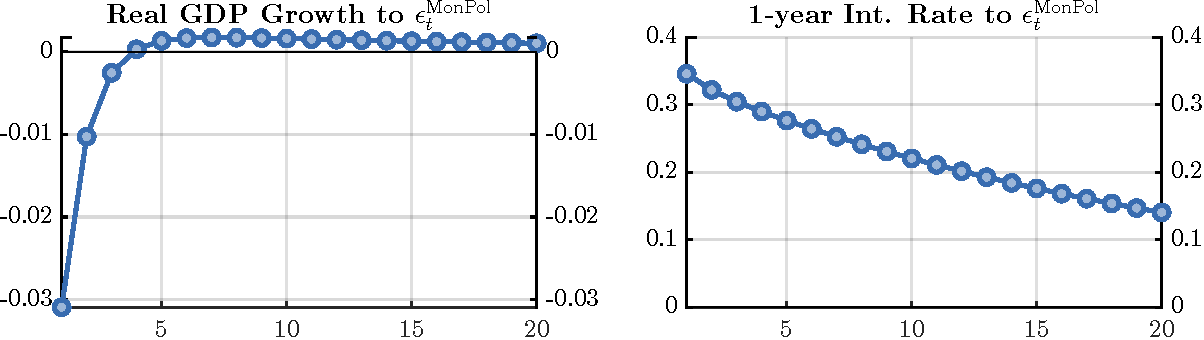
\includegraphics[width=.9\textwidth]{long}
		\end{center}%
		\vspace{0.2cm}
		\caption{\scshape{Impulse Responses to a Monetary Policy Shock:\\ Zero Long-Run Restrictions}}
		\vspace{0.2cm}
		\scriptsize{{\scshape Note.} Point estimates of the impulse responses of the log-difference of US real GDP and the 1-year Treasury bill yield to a contractionary monetary policy shock. Identification: zero long-run (Blanchard-Quah) restriction, which imposes that the monetary policy shock has no long-run cumulative effect on the level of US real GDP ($c_{12}=0$). Bivariate VAR(1) estimated on quarterly US data, 1989:Q1--2019:Q4. Horizon: 20 quarters. Percentage points.}
		\label{fig:long}
	\end{minipage}
\end{figure}

To check that the structural VAR estimated with the above commands is consistent with the assumptions made, note that the $C$ matrix --- the matrix that captures the cumulative long-run effect of shocks on the endogenous variables --- should be lower triangular under the assumptions made above, so that the cumulative effect of $\varepsilon_{t}^{MonPol}$ on the log-difference of US real GDP is zero (long-run monetary neutrality). One way to perform this check is visual: plot the cumulative impulse response of the log-difference of US real GDP, $y_t$, to the monetary policy shock over a long enough horizon, and verify that it converges to zero (the cumulative responses are obtained by summing them along the horizon).

Figure~\ref{fig:longCum} plots the cumulative impulse responses of output growth and the interest rate to the monetary policy shock over a horizon of $150$ quarters. At horizon zero the cumulative responses coincide with the impact responses of Figure~\ref{fig:long}, by construction, since the cumulative sum at the first step is just the impact response itself. As the per-period responses accumulate over longer horizons, the cumulative effect of the shock on the \emph{level} of US real GDP returns to zero (left panel). The reason is that $y_t$ is the log-difference of GDP, so the cumulative sum of its responses measures the total change in the log-level; its convergence to zero is exactly the long-run monetary neutrality imposed by the identifying restriction. The cumulative response of the interest rate is left unrestricted and, in this case, does not converge to zero (right panel).

\vspace{0.2cm}
\begin{figure}[ht!]
	\centering%
	\begin{minipage}[b]{.9\textwidth}
		\begin{center}
		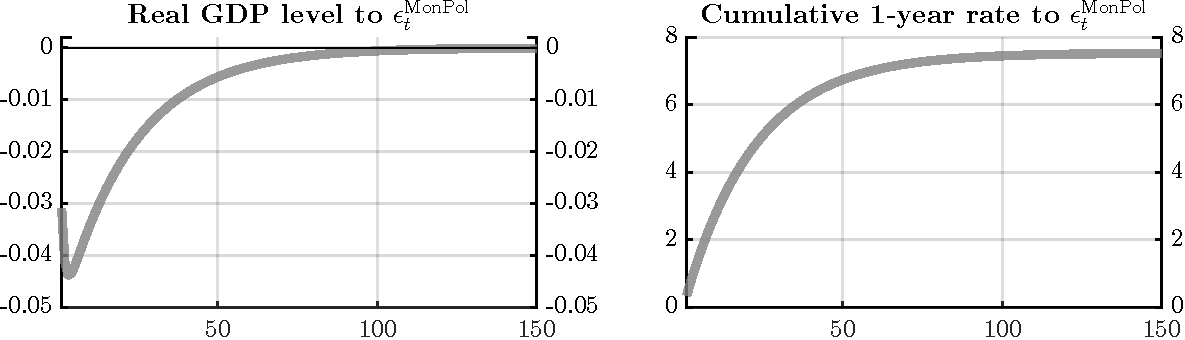
\includegraphics[width=.9\textwidth]{longCum}
		\end{center}%
		\vspace{0.2cm}
		\caption{\scshape{Cumulative Responses to a Monetary Policy Shock:\\ Zero Long-Run Restrictions}}
		\vspace{0.2cm}
		\scriptsize{{\scshape Note.} Cumulative impulse responses of the log-difference of US real GDP (left) and the 1-year Treasury bill yield (right) to a contractionary monetary policy shock. Identification: zero long-run (Blanchard-Quah) restriction. By construction, the cumulative response of the log-difference of US real GDP converges to zero at long horizons, consistent with long-run monetary neutrality. Bivariate VAR(1) estimated on quarterly US data, 1989:Q1--2019:Q4. Horizon: 150 quarters. Percentage points.}
		\label{fig:longCum}
	\end{minipage}
\end{figure}

The check can also be performed algebraically: recalling from equation \eqref{eq:long4} that $C\equiv \left( I-\Phi \right) ^{-1}B$, the $C$ matrix can be printed at screen with the following command:

\begin{matlaboutput}
>> disp((eye(2)-VAR_long.Fcomp)\VAR_long.B)
	0.9224    0.0000
	8.8389    7.5367
\end{matlaboutput}

\noindent As assumed, the $c_{12}$ element is equal to zero.

\subsection{Sign Restrictions}\label{sec:sr}

Zero restrictions can be motivated by economic theory, but theory rarely implies them directly. Even when a theoretical motivation exists, the implied zeros may be hard to defend on substantive grounds. Identification by sign restrictions provides an alternative approach that exploits prior beliefs about the sign that certain shocks should have on certain endogenous variables --- a weaker requirement than imposing exact zeros.

The idea is to impose restrictions on specified orthogonalized impulse response functions. Unlike the identification schemes described above --- where the identifying restrictions select a unique $B$ matrix (i.e.\ a unique rotation $Q$ from the orbit $\{B_0Q : QQ'=I_k\}$; see Box~\ref{box:rotation}) --- sign-restricted VARs are set-identified: the restrictions narrow the parameter space but do not select a unique structural model. The data are potentially consistent with a wide range of $B$ matrices that are all admissible in that they satisfy the sign restrictions --- see \cite{Faust1998}, \cite{CanovaDeNicolo2002}, and \cite{Uhlig2005}.

To fix ideas, consider the sign restrictions needed to separately identify demand and a monetary policy shock, as summarized in Table~\ref{tab:SR}:
\begin{table}[ht!]
	\centering
	\begin{minipage}[b]{.7\textwidth}
		\begin{center}\small
		\begin{tabularx}{\textwidth}{lYY}
		\toprule 
			& \shortstack{Demand\\ Shock} & \shortstack{Monetary\\ Policy Shock} \\
			& ($\varepsilon_{t}^{Demand}$) & ($\varepsilon_{t}^{MonPol}$) \\ \midrule\addlinespace
			Output growth ($y_{t}$) & + & - \\
			Short-term Interest Rate ($r_{t}$) & + & + \\ \bottomrule
		\end{tabularx}%
		\end{center}
		\vspace{0.4cm}
		\caption{\scshape{Sign Restrictions for Demand Shock \\ and Monetary Policy Shock}}
		\vspace{0.2cm}
		\scriptsize{{\scshape Note.} The signs represent restrictions on the elements of the structural impact matrix $B$. `$+$' and `$-$' indicate a positive and negative contemporaneous response, respectively. A demand shock raises both output growth and the short-term interest rate, as monetary policy tightens to contain the expansion. A contractionary monetary policy shock lowers output growth and raises the interest rate, consistent with an unexpected tightening of monetary policy.}
		\label{tab:SR}
	\end{minipage}
\end{table}

\noindent A demand shock ($\varepsilon_{t}^{Demand}$) should lead to an increase in output growth ($y_{t}$) and to an increase in the short-term interest rate ($r_{t}$). The latter sign reflects the assumption that monetary policy responds endogenously to the expansion, as in a standard Taylor-rule framework. By contrast, a contractionary monetary policy shock ($\varepsilon_{t}^{MonPol}$) should lead to a decrease in output growth and an increase in the short-term interest rate, consistent with an unexpected tightening of monetary policy. 



\noindent But how can such restrictions be imposed? The implementation of sign-restriction identification proceeds in three steps.

\begin{enumerate} 
	\item \underline{\textit{Draw an orthogonal matrix ($Q$)}}. \ An orthogonal matrix $Q$ is a real square matrix whose columns form an orthonormal set: each column has unit norm and any two distinct columns are mutually orthogonal.\footnote{To ensure draws are spread uniformly over the orthogonal group, $Q$ is generated via the QR factorization of a random normal matrix. The sign of each column of $Q$ is adjusted so that the corresponding diagonal element of $R$ is positive, which guarantees $\det Q = +1$ and ensures draws are uniformly spread over the rotation subgroup $SO(n)$ in a manner that approximates the Haar measure --- see \citet{Stewart1980}.} Take, for example, two $2\times 1$ vectors $q_{1}$ and $q_{2}$, then the matrix $Q=(q_{1},q_{2})$ is orthogonal if (i) the vectors have unit norm ($\parallel q_{i}\parallel =1$), and (ii) the vectors are mutually orthogonal ($q_{1}^{T}q_{2}=0$). It follows that 
	\begin{equation*}
		QQ'=I_2 \ \ \ \text{and} \ \ \ Q'=Q^{-1}
	\end{equation*}
	Such matrices can be generated by computing the QR factorization of a random matrix with i.i.d.\ standard normal entries --- see the \mc{getqr.m} function and the examples therein.

	\item \underline{\textit{Compute a candidate structural impact matrix ($B_j$)}}. \ Consider the structural impact matrix $B$ corresponding to the Cholesky factor of the reduced-form covariance matrix $\Sigma_{u}$ of our simple bivariate VAR, namely:
	\begin{equation*}
		\Sigma_{u}=PP'.
	\end{equation*}%
	We know from Section~\ref{sec:short} that $B=P$ is the unique lower-triangular structural impact matrix with positive diagonal entries consistent with $\Sigma_u = BB'$; it obtains under the zero contemporaneous restriction $b_{12}=0$. Now note that the following equality holds%
	\begin{equation}\label{eq:Btilde}
		\Sigma_{u}=PP'=PQ_jQ_j'P'=\underset{B_j}{\underbrace{\left( PQ_j\right) }}\underset{B_j'}{\underbrace{\left( PQ_j\right)'}}
	\end{equation}
	where $Q_j$ denotes a randomly drawn orthonormal matrix such that $Q_jQ_j'=I_2$. The defining property of $B_j$ is that, in addition to satisfying \eqref{eq:Btilde}, it is such that the associated structural shocks $\varepsilon_{jt} = B_j^{-1} u_t$ are orthogonal and have unit variance: $E[\varepsilon_{jt}\varepsilon_{jt}'] = I_2$. To verify: $B_j^{-1}\Sigma_u (B_j^{-1})' = B_j^{-1} B_j B_j'(B_j')^{-1} = I_2$. It follows that $B_j$ is a valid candidate structural impact matrix that solves the identification problem. Invertibility of $B_j$ follows because $P$ (a Cholesky factor) and $Q_j$ (an orthogonal matrix) are both invertible, and the product of invertible matrices is invertible. Also note that $B_j$ is not triangular any more. Sign restrictions narrow the set of admissible $B_j$ matrices but generically leave infinitely many. Since the reduced form identifies only $\Sigma_u = BB'$ and not $B$ itself, the data alone cannot resolve this multiplicity. The sign-restriction approach embraces this multiplicity: any $B_j$ consistent with the restrictions is treated as an admissible structural model --- the identified set is the collection of all such $B_j$.

	\item \underline{\textit{Check the sign restrictions}}. \ Sign restrictions identify the VAR by requiring the impulse responses to satisfy specified sign conditions; any $B_j$ consistent with those conditions is treated as a valid structural model. Computationally, a large number of candidate matrices $B_j$ are drawn and those satisfying the sign conditions are retained --- where recall that the $B_j$ matrix contains the impact response of all endogenous variables to all structural shocks. For example, for a given $Q_j$ matrix and associated structural impact matrix $B_j$, the structural representation of our VAR can be written as:
	\begin{equation}
		\left[
		\begin{array}{c}
			y_{t} \\
			r_{t}%
		\end{array}%
		\right] =%
		\begin{bmatrix}
			\phi _{11} & \phi _{12} \\
			\phi _{21} & \phi _{22}%
		\end{bmatrix}%
		\left[
		\begin{array}{c}
			y_{t-1} \\
			r_{t-1}%
		\end{array}%
		\right] +\left[
		\begin{array}{cc}
			b_{j,11} & b_{j,12} \\
			b_{j,21} & b_{j,22}%
		\end{array}%
		\right]
		\begin{bmatrix}
			\varepsilon_{t}^{Demand} \\
			\varepsilon_{t}^{MonPol}%
		\end{bmatrix}%
		,  \label{eq:struct_var_sr}
	\end{equation}%
	where the matrix $B_j = PQ_j$ is now known. We can then check whether the impact response of the two structural shocks to output growth and the short-term interest rate satisfies the sign restrictions. That is:
	\begin{center}\small
		\begin{tabular}{lcc}
			\toprule 
			& Demand Shock & Monetary Policy Shock \\
			& ($\varepsilon_{t}^{Demand}$) & ($\varepsilon_{t}^{MonPol}$) \\ \midrule\addlinespace
			Output growth ($y_{t}$) & $b_{j,11}>0$? & $b_{j,12}<0$? \\
			Short-term Interest Rate ($r_{t}$) & $b_{j,21}>0$? & $b_{j,22}>0$? \\ \bottomrule
		\end{tabular}%
	\end{center}
\end{enumerate}
\bigskip

\noindent If all the elements of $B_j$ satisfy the sign restrictions, we retain the draw and store $PQ_j$; otherwise we discard it and draw a new $Q_j$. After collecting a large number of accepted draws, we have a distribution of $B_j$ matrices --- and of the implied impulse responses, variance decompositions, etc. --- that summarizes the identified set.

\begin{notebox}
\boxentry{Set identification vs.\ point identification}
\textbf{Set identification vs.\ point identification.} \ The identification schemes in Sections~\ref{sec:short} and~\ref{sec:long} are \textit{point-identified}: given the data, a unique $B$ matrix satisfies the identifying restrictions. The Cholesky decomposition delivers exactly one lower-triangular $B$ consistent with $\Sigma_u = BB'$, provided the diagonal entries are required to be positive (a sign normalization that removes the remaining sign ambiguity); the Blanchard-Quah decomposition delivers exactly one $B$ consistent with a lower-triangular long-run matrix $C$. The only source of uncertainty in the resulting impulse responses is therefore sampling variability.

Sign restrictions, by contrast, are \textit{set-identified}: many $B_j$ matrices are simultaneously consistent with the sign restrictions and with the data. Even with an infinite sample, the data alone cannot select among them --- they represent genuinely different structural models, each with its own economic interpretation. This has two important implications. First, summary measures such as the median impulse response across accepted draws need not converge to a unique value as $T\to\infty$, because the identified set remains non-singleton even in the population --- the median describes the location of the identified set, not a point estimate of a unique structural parameter. Second, the width of the credible intervals in sign-restricted VARs reflects both sampling uncertainty \textit{and} the width of the identified set; these two sources of uncertainty cannot be disentangled without imposing additional restrictions --- see \citet{AriasRubioRamirezWaggoner2018} and \citet{GiacominiKitagawa2021} for formal treatments. 

The VAR Toolbox handles parameter uncertainty for sign-restricted VARs through a Bayesian approach: reduced-form parameters are drawn from their posterior distribution, and for each draw the sign-restriction algorithm is applied to find admissible rotations. This is described in Section~\ref{sec:inference}.
\end{notebox}

\noindent \textbf{\sffamily\underline{In MATLAB}.} Sign restrictions in the VAR Toolbox can be implemented with a few lines of code. The restrictions are specified in a $k \times k$ matrix (here $2 \times 2$). Consistent with the notation in equation \eqref{eq:struct_var_sr}, each column collects restrictions for a given structural shock and each row collects restrictions for a given endogenous variable. Entry values are $1$ (positive response required), $-1$ (negative response required), or $0$ (unrestricted). The restrictions described in Table~\ref{tab:SR} can be implemented in MATLAB with the following line of code:

\begin{matlabcode}
% Sign restriction matrix: positive 1, negative -1, unrestricted 0
R = [ 1, -1;  % Real GDP
      1,  1]; % 1-year rate
\end{matlabcode}

\noindent The matrix \mc{R} specifies the sign restrictions as in Table~\ref{tab:SR}. 

It is also useful, though not necessary, to update some fields in the \mc{VARopt} structure. Two fields are specific to sign restrictions: \mc{ndraws} specifies the number of accepted draws the routine needs to find, and \mc{sr\_hor} specifies the number of periods for which the sign restrictions in \mc{R} are required to hold. In this specific example, we set the restrictions to hold for one quarter only (namely, on impact), but they can be specified to hold for longer horizons. The remaining fields, as for other identification schemes, control how the impulse responses are plotted, saved, etc. As most settings have been set for the previous example, it will suffice to run the following lines of code:

\begin{matlabcode}
% Additional options
VARopt.ndraws = 1000;     % number of desired accepted draws
VARopt.sr_hor = 1;        % horizon over which restrictions hold
VARopt.nsteps = 20;       % horizon of impulse responses
VARopt.figsize = [24, 6]; % size of window (figures)
VARopt.snames = {bfeps('Demand'), bfeps('MonPol')}; % shock names
\end{matlabcode}

To implement the approach, as for other identification schemes, set the structure \mc{VARopt.ident = 'sign'}. Then store the restriction matrix in \mc{VARopt.R}, and call \mc{VARmodel}:

\begin{matlabcode}
% Identify with sign restrictions
VARopt.ident = 'sign';
VARopt.R = R;
VAR_sr = VARmodel(X,nlags,detc,VARopt);
\end{matlabcode}

\noindent The structure \mc{VAR\_sr} contains all relevant output. Of particular interest for the discussion in this section are two matrices. The matrix \mc{VAR\_sr.Ball} includes all the accepted draws of $B_j$, and thus has a dimension of $2 \times 2 \times 1000$. Each of the accepted $B_j$, which by definition satisfies the sign restrictions in Table~\ref{tab:SR}, is associated with an impulse response function, stored in the matrix \mc{VAR\_sr.IRall}. 

Figure~\ref{fig:signAll} reports all such responses of the log-difference of US real GDP and the 1-year rate to the monetary policy shock. As the figure makes clear, every accepted draw satisfies the sign restrictions on impact --- GDP falls and the 1-year rate rises --- but the magnitude of the impact responses and the subsequent transmission of the shock differ across draws, reflecting the set-identified nature of the model.

\vspace{0.2cm}
\begin{figure}[ht!]
	\centering%
	\begin{minipage}[b]{.9\textwidth}
		\begin{center}
			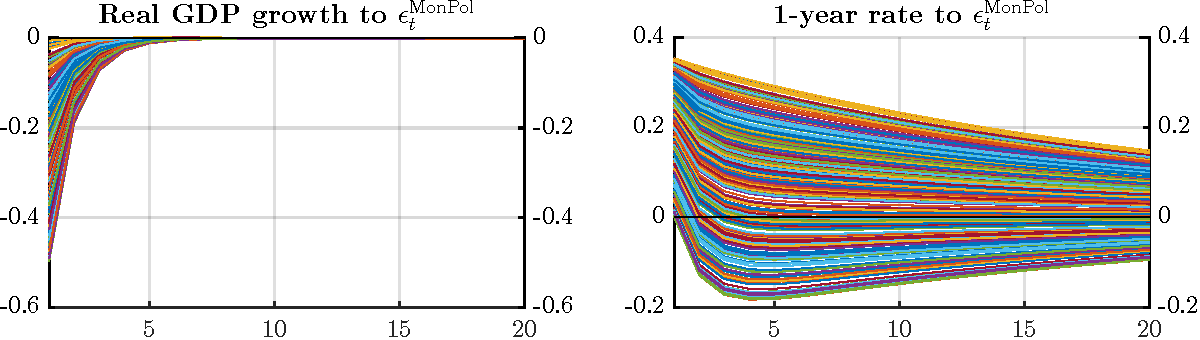
\includegraphics[width=.9\textwidth]{signAll}
		\end{center}%
		\vspace{0.2cm}
		\caption{\scshape{Impulse Responses to a Monetary Policy Shock: \\ All Accepted Draws}}
		\vspace{0.2cm}
		\scriptsize{{\scshape Note.} Full set of accepted impulse responses of the log-difference of US real GDP and the 1-year Treasury bill yield to a contractionary monetary policy shock identified with sign restrictions. Restrictions imposed on impact only: GDP$<0$ and the 1-year rate $>0$ for the monetary policy shock; GDP$>0$ and the 1-year rate $>0$ for the demand shock. Each line corresponds to one of the 1000 accepted draws of the structural impact matrix. Bivariate VAR(1) estimated on quarterly US data, 1989:Q1--2019:Q4. Horizon: 20 quarters. Percentage points.}
		\label{fig:signAll}
	\end{minipage}
\end{figure}

While all accepted draws satisfy the identifying restrictions, it is common to report a summary measure of the identified set. The VAR Toolbox provides two distinct objects for this purpose --- the element-wise median and the Fry-Pagan median-target rotation --- and it is important to understand what each represents. 

The first object, \mc{VAR\_sr.IRmed}, is the \textit{element-wise median} across all \mc{VAR\_sr.IRall}: each entry --- that is, the response of variable $i$ to shock $j$ at horizon $h$ --- is the median of the corresponding entry across all $J$ accepted draws. While \mc{VAR\_sr.IRmed} is a convenient summary of the central tendency of the identified set, the associated impact matrix \mc{VAR\_sr.Bmed} is in general a `\textit{Frankenstein}' object: it corresponds to no accepted draw and will in general not satisfy $\Sigma_u = B_{\text{med}}B'_{\text{med}}$, so it does not represent any valid structural model. The second object, due to \cite{FryPagan2011}, addresses this by selecting, among the accepted draws, the single genuine rotation whose responses are closest to the element-wise median. Box~\ref{box:fp} defines this \textit{median-target} rotation and its relationship to the element-wise median.  

Figure~\ref{fig:sign} plots the two summaries together for the monetary policy shock --- the element-wise median \mc{VAR\_sr.IRmed} and the median-target draw \mc{VAR\_sr.IRfp}. In this bivariate example the two are visually indistinguishable, but they are not identical, and they need not be: as Box~\ref{box:fp} explains, the element-wise median and the median-target rotation differ in general even when the reduced-form parameters are held fixed, and the gap grows with the dimension of the VAR and the width of the identified set.

\vspace{0.2cm}
\begin{figure}[ht!]
	\centering%
	\begin{minipage}[b]{.9\textwidth}
		\begin{center}
			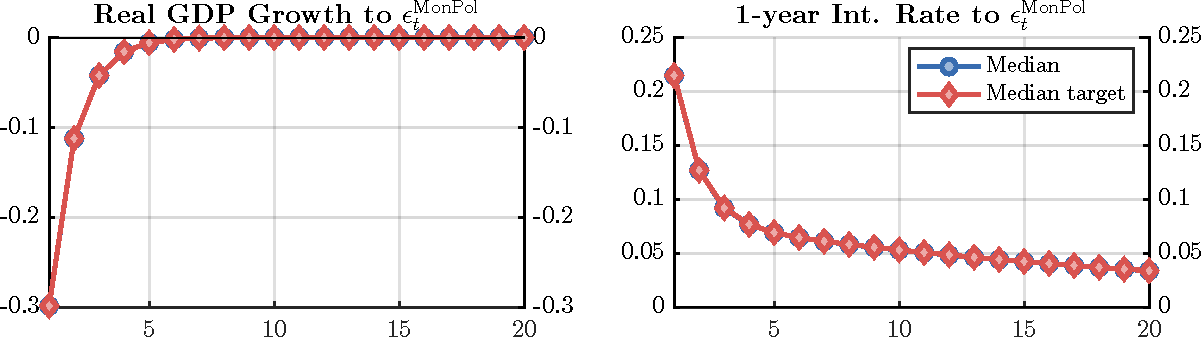
\includegraphics[width=.9\textwidth]{signMed}
		\end{center}%
		\vspace{0.2cm}
		\caption{\scshape{Impulse Responses to a Monetary Policy Shock:\\ Element-Wise Median and Median-Target Rotation}}
		\vspace{0.2cm}
		\scriptsize{{\scshape Note.} Impulse responses of the log-difference of US real GDP and the 1-year Treasury bill yield to a contractionary monetary policy shock identified with sign restrictions. Restrictions imposed on impact only: GDP$<0$ and the 1-year rate $>0$ for the monetary policy shock; GDP$>0$ and the 1-year rate $>0$ for the demand shock. The blue line (circles) is the element-wise median across 1000 accepted draws; the red line (diamonds) is the Fry-Pagan median-target rotation --- the single accepted draw whose responses are closest to the element-wise median. The two are visually indistinguishable here but are not identical (see Box~\ref{box:fp}). Bivariate VAR(1) estimated on quarterly US data, 1989:Q1--2019:Q4. Horizon: 20 quarters. Percentage points.}
		\label{fig:sign}
	\end{minipage}
\end{figure}


\begin{notebox}[label=box:fp]
\boxentry{The Fry-Pagan median-target rotation}
\textbf{The Fry-Pagan median-target rotation.} \ \cite{FryPagan2011} pointed out that the element-wise median \mci{VAR\_sr.IRmed}, though a convenient summary of the identified set, does not correspond to any single structural model: the associated impact matrix \mci{VAR\_sr.Bmed} matches no accepted draw and will in general not satisfy $\Sigma_u = B_{\mathrm{med}}B_{\mathrm{med}}'$. They proposed instead selecting the single accepted draw $B_{j^*}$ whose implied impulse responses are closest to the element-wise median in a least-squares sense:
\begin{equation*}
    j^* = \arg\min_{j} \sum_{h,i,k} \bigl[\mathrm{IR}_{j,hik} - \mathrm{IRmed}_{hik}\bigr]^2.
\end{equation*}
This \textit{median-target} rotation is a genuine structural representation of the VAR: it satisfies all sign restrictions and $\Sigma_u = B_{j^*} B_{j^*}'$ by construction. The VAR Toolbox stores it in \mci{VAR\_sr.Bfp} and \mci{VAR\_sr.IRfp}, with companion fields \mci{VAR\_sr.VDfp} and \mci{VAR\_sr.HDfp} for variance decompositions (Section~\ref{sec:fevd}) and historical decompositions (Section~\ref{sec:hd}). The plotting functions \mci{VARirplot} (as well as \mci{VARvdplot} and \mci{VARhdplot}, which will be discussed in Section~\ref{sec:dynamic}) take whichever field the user explicitly supplies, so the choice between the element-wise median and the Fry-Pagan draw rests with the user. The two options entail different trade-offs. The element-wise median (\mci{.IRmed}, \mci{.VDmed}, \mci{.HDmed}) summarizes the central tendency of the identified set and is easy to compute, but the associated \mci{.Bmed} does not correspond to any accepted draw, VD shares need not sum to one at every horizon, and HD contributions need not exactly reproduce the observed series --- all three being artefacts of element-wise aggregation across draws. The Fry-Pagan draw (\mci{.IRfp}, \mci{.VDfp}, \mci{.HDfp}) is a genuine structural representation: VD shares sum to one and HD contributions reproduce the data exactly, but it selects a single draw from the identified set, which introduces a different form of arbitrariness.

The element-wise median and the median-target rotation differ in general, and the distinction does not depend on whether parameter uncertainty is accounted for. The reason is geometric. The admissible impact matrices satisfy $\Sigma_u = B_j B_j'$, so they lie on a curved set --- the orthonormal rotations of a fixed Cholesky factor of $\Sigma_u$. The element-wise median is taken coordinate by coordinate across draws and is, in general, not a point of this set; this is precisely why \mci{VAR\_sr.Bmed} need not satisfy $\Sigma_u = B_{\mathrm{med}}B_{\mathrm{med}}'$. The median-target rotation returns the single admissible draw whose responses are closest to the element-wise median, which differs from the median itself whenever the median lies off the set. This holds even when \mci{VARopt.inference = 0}: in that case all draws share the OLS estimates $(\hat\Phi,\hat\Sigma_u)$ and vary only through the rotation $B_j$, yet the impulse responses still trace a non-linear set as the rotation varies, so their coordinate-wise median need not be attainable by any single rotation. Accounting for parameter uncertainty (\mci{VARopt.inference = 1}) lets $\Phi_h$ vary across draws as well, adding a second source of dispersion, but it is not what creates the gap. The magnitude of the gap depends on the geometry of the identified set: it is small when the set is tight and low-dimensional --- as in the bivariate example of Figure~\ref{fig:sign}, where the two summaries are visually indistinguishable --- and grows with the dimension of the VAR and the width of the identified set. Note that the running example of this section sets \mci{VARopt.inference = 0} (Section~\ref{sec:inference}), so the comparison in Figure~\ref{fig:sign} isolates identification (rotation) uncertainty; the difference between the two summaries is therefore not an artefact of parameter uncertainty.
\end{notebox}

\subsection{Narrative Sign Restrictions}\label{sec:narr}

Sign restrictions, as described in Section~\ref{sec:sr}, restrict the \textit{sign} of the impulse responses over some horizon. A large set of rotation matrices $Q_j$ can satisfy the sign restrictions, producing a correspondingly wide set of admissible structural impact matrices $B_j$ and, consequently, wide credible sets for impulse responses. \cite{AntolinDiazRubioRamirez2018} propose to sharpen identification by incorporating \textit{narrative restrictions} --- additional constraints tied to specific, well-documented historical events. The insight is that historical records (monetary policy announcements, oil supply disruptions, fiscal interventions) carry information about the sign or relative magnitude of a structural shock at a particular date. Restricting the model to be consistent with that information reduces the set of admissible rotations and, in practice, substantially tightens inference.

To fix ideas, suppose that in a particular quarter there was an unambiguous monetary policy tightening. This historical knowledge carries two pieces of information. First, the monetary policy shock must have been positive in that quarter --- the direction of the move is known from the historical record. Second, if historical records further suggest that no major competing shock was operating simultaneously, then monetary policy was plausibly the dominant driver of the policy rate in that quarter. These two pieces of information motivate the two types of narrative restriction defined by \cite{AntolinDiazRubioRamirez2018}. Let $\varepsilon_{jt} = B_j^{-1}u_t$ denote the vector of structural shocks under candidate $B_j$, where $j$ indexes a particular draw.
\begin{itemize}

\item \underline{\textit{Sign restriction (type 1).}} At date $t^*$, the $m$-th structural shock $\varepsilon_{j,m,t^*}$ must have a specified sign:
\begin{equation}
    s \cdot \varepsilon_{j,m,t^*} > 0, \qquad s \in \{+1, -1\}.
    \label{eq:narr_type1}
\end{equation}
In the example above, this encodes the knowledge that the monetary policy shock was positive ($s=+1$) in the quarter of the unambiguous tightening. \medskip

\item \underline{\textit{Dominance restriction (type 2).}} At date $t^*$, the contribution of shock $m$ to the unexpected movement in variable $i$ must exceed the combined contribution of all other shocks:
\begin{equation}
    \bigl|b_{j,im}\,\varepsilon_{j,m,t^*}\bigr| > \sum_{k \neq m} \bigl|b_{j,ik}\,\varepsilon_{j,k,t^*}\bigr|,
    \label{eq:narr_type2}
\end{equation}
where $b_{j,im}$ is the $(i,m)$ element of $B_j$. In the example above, this encodes the knowledge that monetary policy was the dominant driver of the policy rate in that quarter. 
\end{itemize}

\noindent Both restrictions are applied as additional acceptance criteria \textit{after} a rotation satisfying the sign constraints has been found. A draw $j$ that passes the sign restrictions but fails any narrative restriction is discarded. Because narrative restrictions are layered on top of the sign constraints, the number of accepted draws can only decrease or remain unchanged relative to the sign-only baseline. A substantial decrease indicates that the historical episodes are genuinely informative and narrow the identified set; little or no decrease indicates that the narrative restrictions add little beyond what the sign constraints already impose.\footnote{The toolbox imposes the narrative restrictions by equal-weight acceptance-rejection: every accepted draw enters the reported set with the same weight. When parameter uncertainty is accounted for (\mc{VARopt.inference = 1}), this is not the posterior derived by \cite{AntolinDiazRubioRamirez2018}. Because the probability that a sign-admissible rotation also satisfies the narrative restrictions varies with the reduced-form parameters $(\Phi,\Sigma_u)$, plain acceptance-rejection reweights the reduced-form posterior toward regions where the narrative restrictions are easier to satisfy. The correct posterior is recovered by importance sampling: each accepted draw receives a weight proportional to the reciprocal of that probability, estimated by Monte Carlo over rotations at each reduced-form draw, and the draws are resampled accordingly. The toolbox follows the common convention of omitting this reweighting. The two schemes coincide when parameter uncertainty is switched off (\mc{VARopt.inference = 0}, as in the example of this section), since the importance weight is then constant across draws.}

\noindent \textbf{\sffamily\underline{In MATLAB}.} Narrative sign restrictions are implemented via the same \mc{VARmodel} call used for standard sign restrictions. The second argument \mc{R} accepts either a plain sign-restriction matrix --- in which case \mc{VARmodel.m} behaves identically to its non-narrative version --- or a struct that combines sign and narrative restrictions. When \mc{R} is a struct, it has to contain three fields:
\begin{itemize}
    \item \mc{R.sign}: the sign-restriction matrix, in the same format as the \mc{R} matrix of Section~\ref{sec:sr}.

    \item \mc{R.narr\_sign}: encodes Type~1 restrictions (sign of the shock at a specific date). It is a struct with three row vectors. \mc{shock} is the index for the column of $B$ identifying the structural shock to restrict. \mc{period} identifies the quarter in which the shock to be restricted occurred, indexed against the input data passed to \mc{VARmodel}. It accepts either a date string (e.g.\ \mc{'1994q1'}, which requires \mc{VARopt.dates} to be set) or the integer row of that quarter in the input data; the two forms are equivalent and point to the same observation. The toolbox handles the internal alignment with the residual sample, so a quarter falling inside the first $p$ rows --- absorbed as initial lags and hence without an associated shock --- is rejected with an error. \mc{sign} specifies the required direction of the shock: $+1$ for a positive realization, $-1$ for a negative one. Multiple Type~1 restrictions are stacked as additional rows in each vector.

    \item \mc{R.narr\_dom}: encodes Type~2 restrictions (dominance of the shock at a specific date). It is a struct with three row vectors: \mc{shock} and \mc{period} follow the same conventions as in \mc{R.narr\_sign}. The third row vector \mc{var} is the index of the variable that the shock must dominate --- the shock's contribution to the reduced-form residual of that variable must exceed the combined contribution of all other shocks. Multiple Type~2 restrictions are stacked as additional rows.
\end{itemize}
Both \mc{R.narr\_sign} and \mc{R.narr\_dom} are optional; omit either field to skip that class of restrictions.  The code below illustrates the implementation for the bivariate monetary VAR of Section~\ref{sec:sr}, using two historical episodes chosen to illustrate both the power and the limits of narrative identification at quarterly frequency.
\begin{itemize}
    \item \underline{\textit{1994:Q1 --- sign and dominance.}} Greenspan's February 4 hike was an unambiguous surprise tightening in a quarter with no major competing macroeconomic disturbance. Historical records leave little doubt that the monetary policy shock was positive that quarter, motivating a Type~1 restriction. Since no major non-monetary shock was operating simultaneously, monetary policy was plausibly the dominant driver of the variation in the 1-year yield, motivating a Type~2 restriction as well.\medskip

    \item \underline{\textit{2001:Q1 --- sign only.}} The January 3 unscheduled inter-meeting cut was an unambiguous easing surprise --- historical records clearly place the monetary policy shock in negative territory, motivating a Type~1 restriction. A Type~2 restriction is not warranted, however. The quarter also contains a large concurrent non-monetary disturbance: the dot-com bust and the peak of the business cycle in March, as dated by the NBER.
\end{itemize}
These restrictions can be implemented in MATLAB as follows:

\begin{matlabcode}
% Sign restrictions
R.sign = [ 1, -1;  % Real GDP
           1,  1]; % 1-year rate

% Sign of MP shock for both episodes
R.narr_sign.shock  = [2;        2      ];
R.narr_sign.period = {'1994q1'; '2001q1'};
R.narr_sign.sign   = [1;       -1      ];

% MP shock is the dominant driver of i1yr only in 1994q1
R.narr_dom.shock  = [2;        ];
R.narr_dom.period = {'1994q1'; };
R.narr_dom.var    = [2;        ];
\end{matlabcode}

\noindent With the \mc{R} struct in place, it must be assigned to the \mc{VARopt} structure, together with a few additional options.

\begin{matlabcode}
% Set options for the sign restriction routine
VARopt.R 	   = R;      % assign R to VARopt
VARopt.dates   = dates;  % date strings aligned with VAR input data
VARopt.sr_draw = 500000; % total number of draws to attempt
VARopt.figsize = [24, 6];
VARopt.snames  = {bfeps('Demand'), bfeps('MonPol')};
\end{matlabcode}

\noindent The two key fields are \mc{VARopt.R}, which assigns the restriction struct, and \mc{VARopt.dates}, which supplies the date strings that align \mc{R} with the VAR input data. Note that \mc{ndraws} (set earlier to 1000) specifies the number of \textit{accepted} draws to collect, while \mc{sr\_draw} specifies the total number of \textit{candidate} draws to attempt. Because narrative restrictions are more stringent, a larger candidate pool is needed.\footnote{\mci{sr\_draw} imposes a hard ceiling on the total number of candidate draws, preventing the algorithm from running indefinitely when the restrictions are very tight and accepted draws are rare.} The ratio of accepted to total draws also signals how informative the narrative restrictions are: a low ratio indicates that the restrictions substantially constrain the identified set.

With the options set, the narrative-restriction identification is run as usual through the \mc{VARmodel} call:

\begin{matlabcode}
% Identify with sign + narrative restrictions
VAR_nsr = VARmodel(X, nlags, detc, VARopt);
\end{matlabcode}

\noindent where recall that the field \mc{VARopt.ident='sign'} had been already set in the sign restrictions example. The output \mc{VAR\_nsr} has the same structure as \mc{VAR\_sr} from Section~\ref{sec:sr}. Adding narrative restrictions tightens identification at the cost of a lower acceptance rate: in this example, the acceptance rate falls from 73.9\% under sign restrictions alone to 31.9\% under sign plus narrative restrictions, as the additional constraints screen out a substantial share of sign-consistent rotations. The acceptance rates are stored in \mc{VAR\_sr.accept\_rate} and \mc{VAR\_nsr.accept\_rate}, respectively.

Figure~\ref{fig:narr} compares impulse responses to a monetary policy shock under sign restrictions alone (blue) and under sign plus narrative restrictions (red). Shaded areas show the set spanned by all accepted draws; solid lines show the element-wise median across draws. Two effects are visible. First, the narrative restrictions shrink the identified set: the red shaded area is noticeably narrower than the blue one. Second, the median responses shift --- narrative information changes the central estimate, not only its precision. The additional restrictions screen out rotations that are sign-consistent but historically at odds with the narrative evidence, leaving a smaller and differently centred set of admissible impulse responses.

\vspace{0.2cm}
\begin{figure}[ht!]
	\centering%
	\begin{minipage}[b]{.9\textwidth}
		\begin{center}
			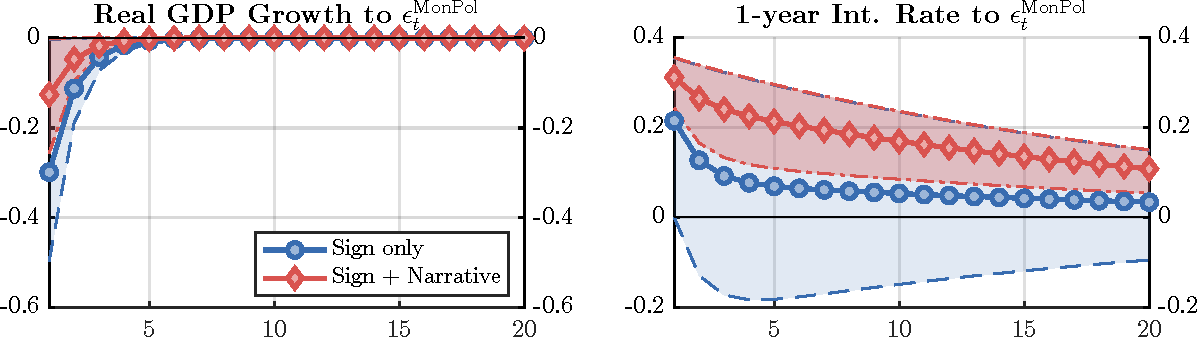
\includegraphics[width=.9\textwidth]{narr}
		\end{center}%
		\vspace{0.2cm}
		\caption{\scshape{Impulse Response to a Monetary Policy Shock:\\ Sign Only vs.\ Narrative Sign Restrictions}}
		\vspace{0.2cm}
		\scriptsize{{\scshape Note.} Impulse responses of log-differenced US real GDP (left) and the 1-year Treasury yield (right) to a contractionary monetary policy shock. Blue: sign restrictions only (shaded area: all accepted draws; solid line: median). Red: sign restrictions augmented with narrative restrictions. Narrative episodes: 1994:Q1 (Greenspan's February 1994 hike, Type~1 and Type~2 restrictions) and 2001:Q1 (January 3 unscheduled inter-meeting cut, Type~1 restriction only). Bivariate VAR(1) estimated on quarterly US data, 1989:Q1--2019:Q4. Horizon: 20 quarters.}
		\label{fig:narr}
	\end{minipage}
\end{figure}

Figure~\ref{fig:narrShockDist} shows the distribution of the identified monetary policy shock at each narrative date, across all accepted draws under sign restrictions alone (blue) and under sign plus narrative restrictions (red). Each panel corresponds to one narrative event, and the shift from blue to red reveals which restriction is binding and how it alters the set of admissible draws. In 1994:Q1, the sign-only distribution is already entirely in positive territory: the sign restrictions alone were sufficient to pin down the direction of the shock in that quarter, so the Type~1 narrative restriction (which requires a positive shock) does not eliminate any additional draws and is not the binding constraint. What does bite is the dominance restriction, which requires the monetary policy shock to be the largest contributor to the policy rate in that quarter. This additional requirement screens out draws that, while sign-consistent, attribute a larger share of the policy-rate move to the demand shock; the result is that the red distribution is shifted toward larger positive values relative to the blue.

\vspace{0.2cm}
\begin{figure}[h!] 
	\centering%
	\begin{minipage}[b]{.9\textwidth}
		\begin{center}
			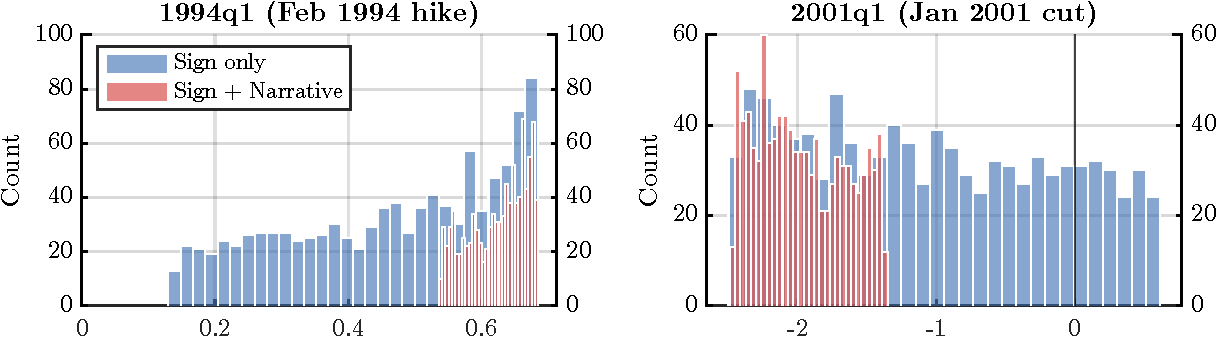
\includegraphics[width=.9\textwidth]{narr_ShockDist}
		\end{center}%
		\vspace{0.2cm}
		\caption{\scshape{Distribution of the Monetary Policy Shock:\\ Sign Only vs.\ Narrative Sign Restrictions}}
		\vspace{0.2cm}
		\scriptsize{{\scshape Note.} Distribution of the identified monetary policy shock across all accepted draws at 1994:Q1 (left) and 2001:Q1 (right). Blue: sign restrictions only. Red: sign restrictions augmented with narrative restrictions. The narrative restriction requires a positive shock in 1994:Q1 and a negative shock in 2001:Q1. A dominance requirement is imposed at 1994:Q1 only. Bivariate VAR(1) estimated on quarterly US data, 1989:Q1--2019:Q4.}
		\label{fig:narrShockDist}
	\end{minipage}
\end{figure}

In 2001:Q1, the sign-only distribution is predominantly negative --- consistent with the historical narrative of a policy easing --- but retains a non-negligible right tail of positive realizations. These are draws for which the sign restrictions happened to be satisfied yet the shock took the wrong sign in that quarter. The Type~1 narrative restriction, which requires a negative monetary policy shock at 2001:Q1, removes exactly this tail: the red distribution is entirely negative, and its support is tighter than the blue.

\subsection{External Instruments (or Proxies)}\label{sec:iv}

External instruments identification was introduced by \cite{StockWatson2012} and \cite{MertensRavn2013}. It is also known in the literature as the \textit{proxy SVAR}, a term that reflects the role of the instrument as a proxy for the unobserved structural shock. It uses standard instrumental variable techniques to isolate the variation in the VAR reduced-form residuals that is due to the structural shock of interest. The approach requires an instrument correlated with the structural shock of interest and orthogonal to all other structural shocks.

For the example in this section, assume that the data are driven by a monetary policy shock, as well as another shock (or a combination of shocks) that we leave unidentified. Also assume that a valid instrument ($z_{t}$) for the monetary policy shock exists, namely that $z_{t}$ is correlated with $\varepsilon_{t}^{MonPol}$ and uncorrelated with the other shock $\varepsilon_{t}^{Other}$. More formally, $z_t$ satisfies the following properties:
\begin{eqnarray}
	\mathbb{E}\left[ \varepsilon_{t}^{MonPol}z_{t}\right]  &=&\alpha \neq 0, \label{eq:instr_rel}\\
	\mathbb{E}\left[\varepsilon_{t}^{Other}z_{t}\right] &=&0,
	\label{eq:instr_iv}
\end{eqnarray}%
The condition $\alpha \neq 0$ is the \textit{relevance} condition; it ensures the instrument has nonzero correlation with the shock of interest. If such an instrument exists, one can identify the impact response of each endogenous variable to the monetary policy shock. That is, one can identify one column of the $B$ matrix --- here, the first column, which corresponds to the monetary policy shock, namely:\footnote{Note that in the sign-restriction example of Section~\ref{sec:sr}, the monetary policy shock occupied the second column; the ordering is a modeling choice with no substantive implications.}
\begin{equation}
	B=\left[
	\begin{array}{cc}
		b_{11} & - \\
		b_{21} & -%
	\end{array}%
	\right]
	\label{eq:column_iv}
\end{equation}

The intuition is as follows. Recall that the reduced-form residuals $u_{yt}$ and $u_{rt}$ are a linear combination of two orthogonal shocks $\varepsilon_{t}^{MonPol}$ and $\varepsilon_{t}^{Other}$:
\begin{equation}
	\begin{array}{c}
		u_{yt}=b_{11}\varepsilon_{t}^{MonPol}+b_{12}\varepsilon_{t}^{Other},
		\\
		u_{rt}=b_{21}\varepsilon_{t}^{MonPol}+b_{22}\varepsilon_{t}^{Other}.%
	\end{array}
	\label{eq:red_resid_iv}
\end{equation}%
It is therefore possible to isolate the variation in $u_{yt}$ attributable to the shock of interest by regressing $u_{yt}$ on the instrument $z_{t}$:
\begin{equation}
	u_{yt}=\beta z_{t}+\xi _{t},
	\label{eq:first_stage}
\end{equation}%
The fitted values of this first-stage regression $\hat{u}_{yt}=\hat{\beta}z_t$ capture the variation in $u_{yt}$ attributable to the monetary policy shock. As $z_t$ is orthogonal to $\varepsilon_{t}^{Other}$, the variation in $u_{yt}$ attributable to the other shock (namely, the component $b_{12}\varepsilon_{t}^{Other}$) ends up in the residual $\xi_t$. By projecting the residuals of the interest rate equation $u_{rt}$ on the fitted values of the previous regression $\hat{u}_{yt}$, it is possible to obtain a consistent estimate of the ratio $b_{21}/b_{11}$:
\begin{equation}
	u_{rt}=\underset{b_{21}/b_{11}}{\underbrace{\gamma }}\hat{u}_{yt}+\zeta _{t},
	\label{eq:second_stage}
\end{equation}%

Because $\hat{u}_{yt}$ inherits orthogonality to $\varepsilon_{t}^{Other}$ from the first-stage projection, the variation in $u_{rt}$ attributable to the other shock is absorbed into the residual $\zeta_t$, while the fitted values $\hat{\gamma}\hat{u}_{yt}$ isolate the variation in $u_{rt}$ attributable to the monetary policy shock. If we normalize $b_{11}=1$ (that is, if we consider a monetary policy shock that raises the log-difference of US real GDP by 1 percentage point) we can easily recover $b_{21}=\gamma$.\footnote{In the VAR Toolbox, the impulse responses are further normalized to match the standard deviations of the shocks, as explained in \cite{GertlerKaradi2015}. See Appendix~\ref{sec:app_gk} for details.} The procedure described in this section thus provides an estimate of the first column of $B$ up to a scaling factor:
\begin{equation}
	B=\left[
	\begin{array}{cc}
		1 & - \\
		\gamma & -%
	\end{array}%
	\right]
	\label{eq:column_iv_norm}
\end{equation}
which can then be used to compute the impulse response to the monetary policy shock as described above.

\noindent \textbf{\sffamily\underline{In MATLAB}.} As for other identification schemes, set the \mc{VARopt.ident} field to identify the VAR with the external instrument. The mnemonic for the external instruments identification is the string \mc{\textcolor{matlabpurple}{'iv'}}. Unlike the other identification schemes, \mc{'iv'} requires a second mandatory input: the external instrument itself must be supplied through the \mc{VARopt.IV} field. Without it the routine has no instrument to project the reduced-form residuals on, and identification cannot proceed. The remaining field set below, \mc{VARopt.snames}, is optional and is used only when plotting and saving the impulse responses. 
 
\begin{matlabcode}
% Set identification to 'iv' and set instrument
VARopt.ident    = 'iv';
VARopt.IV       = mps;
VARopt.snames   = {bfeps('MonPol'), bfeps('Other')};
\end{matlabcode}

\begin{notebox}[label=box:mps]
\boxentry{Warning: the instrument \protect\texttt{mps} is fictitious (do not replicate)}
\textbf{\lapisbox[color=BoEred]{Warning:} the instrument \mci{mps} used in this example is fictitious and must never be replicated in applied work.} \ A valid external instrument must satisfy two conditions: \textit{relevance} (correlation with the structural shock of interest) and \textit{exogeneity} (orthogonality to all other structural shocks). A canonical example meeting both conditions is the high-frequency monetary policy surprise of \cite{GertlerKaradi2015}, constructed from narrow windows around FOMC announcements to isolate exogenous policy movements from the broader macroeconomic environment.

The series \mci{mps} used here is constructed by adding random noise to the monetary policy shock derived from the sign-restriction exercise of Section~\ref{sec:sr}: \mci{mps = [NaN; eps\_sign(:,2)] + noise}, where \mci{noise} $\sim \mathcal{N}(0,1)$. This makes no economic sense as an instrument, but it delivers something that works mechanically. The sole reason for using it is that the bivariate VAR(1) estimated throughout this handbook is too parsimonious to deliver credible results with any real-world instrument. The example is intended to illustrate the \textit{mechanics} of proxy SVAR identification --- how the code is set up, how the output is structured, and how the results compare to other approaches --- not to serve as a model for instrument construction.
\end{notebox}

The identification with external instruments is then implemented with the usual \mc{VARmodel} call:

\begin{matlabcode}
% Identify with external instrument
VAR_iv = VARmodel(X,nlags,detc,VARopt);
\end{matlabcode}

\noindent The \mc{VAR\_iv} structure is populated with \mc{VAR\_iv.B} consistent with the IV identification scheme and with \mc{VAR\_iv.FirstStage}, a structure containing the first-stage regression results. As in a standard instrumental variable approach, the F-statistic of the first stage is important to assess instrument relevance. Only the first column of the $B$ matrix is identified (the monetary policy shock); the second column is set to zero as a placeholder, since the other shock is left unidentified.\footnote{Setting the unidentified columns to zero rather than setting them to NaN ensures that the plotting functions (\mci{VARirplot.m}, \mci{VARvdplot.m}, etc.) do not produce errors when iterating over all columns of $B$.} As usual, the $B$ matrix can be printed as follows:

\begin{matlaboutput}
>> disp(VAR_iv.B)
	0.5375   0
	0.1538   0
\end{matlaboutput}

\noindent A practical limitation of the exogeneity condition is that it is \textit{not testable} in the exactly-identified case --- that is, when there is one instrument for one structural shock. Since exogeneity requires orthogonality between the instrument and all other structural shocks, and these shocks are unobserved, there is no sample analog from which to construct a test. In the over-identified case (more instruments than structural shocks to identify), the over-identifying restrictions can be tested via the Sargan-Hansen $J$-test in a GMM framework (the Sargan test is a special case under homoskedasticity); these provide indirect evidence on instrument validity. See \citet{StockWrightYogo2002} for an overview of weak-instrument and instrument-validity issues in IV estimation.

\begin{notebox}
\boxentry{Assessing instrument strength: the first-stage $F$-statistic}
\textbf{Assessing instrument strength: the first-stage F-statistic.} \ The F-statistic of the first-stage regression tests whether the instrument is sufficiently correlated with the reduced-form residual of interest. A weak instrument --- one with low partial correlation with the target variable --- produces biased and imprecise IV estimates, regardless of whether the exogeneity condition is satisfied. The conventional rule of thumb, due to \cite{StockYogo2002}, is that the first-stage F-statistic should exceed 10. This threshold applies to the benchmark case of one instrument and one endogenous regressor at a 5\% size-distortion tolerance; the appropriate critical value differs with the number of instruments and regressors --- see \citet{StockYogo2002} for the full table. Below that threshold, the instrument is considered weak and the two-stage estimates are unreliable.

\cite{GertlerKaradi2015} report a first-stage F-statistic well above 10 for their high-frequency monetary policy surprise instrument, confirming its relevance. In the VAR Toolbox, the first-stage F-statistic is stored in \mci{VAR\_iv.FirstStage.F} and can be inspected directly:
\begin{matlaboutput}
>> disp(VAR_iv.FirstStage.F)
   13.2691
\end{matlaboutput}
\noindent In this example, the F-statistic of 13.27 exceeds the conventional threshold of 10, suggesting the instrument has adequate relevance.
\end{notebox}

The two-stage IV procedure delivers only the identified column of $B$, that is, the contemporaneous (impact, $h=0$) responses of the two variables to the monetary policy shock. These impact responses are the stars in Figure~\ref{fig:iv}. From the impact responses onward, no further identifying information is needed: the responses at horizons $h \geq 1$ are obtained by propagating the impact vector through the estimated reduced-form VAR dynamics, exactly as for any other identification scheme described above. In other words, identification pins down where the impulse response starts, and the estimated VAR coefficients determine how it propagates over time. The full set of responses, from $h=0$ to the chosen horizon, is stored in \mc{VAR\_iv.IR}. Figure~\ref{fig:iv} reports the resulting impulse responses to the identified monetary policy shock.

\vspace{0.2cm}
\begin{figure}[ht!]
	\centering%
	\begin{minipage}[b]{.9\textwidth}
		\begin{center}
			
\includegraphics[width=.9\textwidth]{iv}
		\end{center}%
		\vspace{0.2cm}
		\caption{\scshape{Impulse Responses to a Monetary Policy Shock}}
		\vspace{0.2cm}
		\scriptsize{{\scshape Note.} Point estimates of the impulse responses of the log-difference of US real GDP and the 1-year Treasury bill yield to a contractionary monetary policy shock identified with an external instrument (proxy SVAR). The impact responses (marked with stars) are recovered via a two-stage IV regression of the reduced-form residuals on the instrument; subsequent responses are propagated through the estimated VAR dynamics. Bivariate VAR(1) estimated on quarterly US data, 1989:Q1--2019:Q4. Horizon: 20 quarters. Percentage points.}
		\label{fig:iv}
	\end{minipage}
\end{figure}

\subsection{Combining Sign Restrictions and External Instruments}\label{sec:iv_sign}

The external instruments and sign restriction identification approaches can be combined as proposed by \cite{CesaBianchiSokol2021}. The main idea of this approach is to identify one (or more) shocks with external instruments and the remaining shocks (or a subset of them) with sign restrictions. The motivation is practical: in many applications the researcher has a credible instrument for one shock of interest --- typically the monetary policy shock --- but no equally credible instrument for the other shocks driving the system. Rather than discarding the instrument and identifying all shocks with sign restrictions, or leaving the remaining shocks unidentified, this approach uses the instrument to point-identify the shock for which it is available and sign restrictions to set-identify the rest. The two strategies are complementary: the instrument delivers a sharp, point estimate for one column of $B$, while sign restrictions impose weaker, inequality-based constraints on the remaining columns.

This section builds on the example used in the previous section, where a monetary policy shock is identified with external instruments and a second shock is left unidentified. Unlike the previous section, assume here that the second shock driving the data is a demand shock, so that the system is now fully identified rather than only partially. Since the monetary policy shock is point-identified with the external instrument, no further restrictions are needed on its column of $B$; sign restrictions are therefore required only for the demand shock, as discussed in Section~\ref{sec:sr}. Table~\ref{tab:iv_SR} summarizes the identifying restrictions on the elements of the structural impact matrix $B$, noting that the first column is identified with the external instrument while the second is restricted in sign:

\begin{table}[ht!]
	\centering
	\begin{minipage}[b]{.9\textwidth}
		\begin{center}\small
		\begin{tabular}{lcc}
			\toprule 
			& Monetary Policy Shock& Demand Shock  \\
			& ($\varepsilon_{t}^{MonPol}$) & ($\varepsilon_{t}^{Demand}$) \\ \midrule\addlinespace
			Output growth ($y_{t}$) & Ext. Instrument & + \\
			Short-term Int. Rate ($r_{t}$) & Ext. Instrument & + \\ \bottomrule
		\end{tabular}%
		\end{center}
		\vspace{0.4cm}
		\caption{\scshape{Restrictions for Monetary Policy and Demand Shocks}}
		\vspace{0.2cm}
		\scriptsize{{\scshape Note.} The signs represent restrictions on the elements of the structural impact matrix $B$. `$+$' and `$-$' indicate sign restrictions on the contemporaneous response. `Ext.\ Instrument' indicates identification via an external instrument proxy.}
		\label{tab:iv_SR}
	\end{minipage}
\end{table}

To see how to combine the external instrument and sign restrictions approaches, start by partitioning the matrix $B$ into a column vector $B^{IV}$, which captures the impact of the monetary policy shock, and a column vector $B^{SR}$, which captures the impact of the demand shock:
\begin{equation}
	B=\left[
	\begin{array}{cc}
		B^{IV} & B^{SR}%
	\end{array}%
	\right] .  \label{eq:B_partitioned}
\end{equation}%
where $B^{IV} $ and $B^{SR}$ are $2\times 1$ vectors.\footnote{Note that both $B^{IV}$ and $B^{SR}$ can be matrices, i.e.\ can include more than one shock, as in the original paper by \cite{CesaBianchiSokol2021}.} Assuming that a valid instrument for the monetary policy shock exists, the first column of the $B$ matrix ($B^{IV}$) is point-identified as explained in the previous section.

We now show how to combine the external instruments identification approach with a standard sign restriction approach to identify the remaining structural shock ($\varepsilon_{t}^{Demand}$) conditional on the shock identified with the external instrument ($\varepsilon_{t}^{MonPol}$). To identify $B^{SR}$\ (i.e.\ the contemporaneous impact of the demand shock)\ we proceed as follows. First, using (\ref{eq:B_partitioned}), re-write the covariance matrix of the reduced-form residuals as:%
\begin{equation}
	\Sigma_{u}=BB'=\left[
	\begin{array}{cc}
		B^{IV} & B^{SR}%
	\end{array}%
	\right] \left[
	\begin{array}{cc}
		B^{IV} & B^{SR}%
	\end{array}%
	\right]'.  \label{eq:cov_partitioned}
\end{equation}%
As we have seen above, this decomposition of the covariance matrix is not unique. Let $P$ be the Cholesky decomposition of the covariance matrix $\Sigma_{u}$, and let $Q_j$ be a randomly drawn orthonormal matrix (where, as before, $j$ denotes a random draw) such that $Q_jQ_j'=I_k$, then:
\begin{equation}
	\Sigma_{u}=PP'=PQ_jQ_j'P'=\left( PQ_j\right) \left(
	PQ_j\right)'
\end{equation}%
Similarly to the sign restriction procedure, the identification strategy described in this section consists in constructing a large number of orthonormal matrices $Q_j$ that satisfy the following condition:
\begin{equation}
	PQ_j=\left[
	\begin{array}{cc}
		B^{IV} & B_j^{SR}
	\end{array}%
	\right]
\end{equation}%
where $B^{IV}$ is point-identified with the external instrument and $B_j^{SR}$ is set-identified with the sign restrictions. Thus, the main difference with the standard sign restriction procedure lies in the construction of the $Q_j$ matrix. Instead of obtaining $Q_j$ from a QR factorization of a random matrix with elements from the standard normal distribution, here we construct the $Q_j$ matrix sequentially, with the following two steps:

\begin{enumerate}
	\item Find a unit vector $Q^{IV}$ of dimension $k \times 1$ that rotates the first column of $P$ into the vector $B^{IV}$. That is, we find a $k\times 1$ unit vector $Q^{IV}$ such that the following equality holds:%
	\begin{equation}
		PQ^{IV}=B^{IV}
	\end{equation}
	
	\item Given $Q^{IV}$, build the remaining column of an orthonormal $2 \times 2$ matrix $Q_j$ following a standard Gram-Schmidt process.\footnote{Let $j$ index the columns of $Q.$ Let $Q_{j-1}$ denote the first $j-1$
		columns of $Q$, such that $Q_{2-1}=Q_{1}=q_{1}.$ Let $x_{j}$ be a draw from
		a Normal distribution on $\mathbb{R}^{k}.$ Then the $j-$th column of $Q$ can
		be constructed as: %
		$q_{j}=\left( I_{k}-Q_{j-1}Q_{j-1}'\right) x_{j}/\left\Vert\left( I_{k}-Q_{j-1}Q_{j-1}'\right) x_{j}\right\Vert$.%
	} That is, find a $(k \times 1)$ vector $Q^{SR}_j$ such that the following equality holds:%
	\begin{equation}
		\begin{bmatrix}
			Q^{IV} & Q^{SR}_j%
		\end{bmatrix}%
		\begin{bmatrix}
			Q^{IV} & Q^{SR}_j%
		\end{bmatrix}%
		'=Q_jQ_j'=I.
	\end{equation}%
\end{enumerate}

\noindent As in the standard sign restriction procedure, the matrix $B_j=PQ_j$ then represents a candidate structural representation because:
\begin{equation}
		\Sigma_u = 
		\begin{bmatrix}
			B^{IV} & B_j^{SR}%
		\end{bmatrix}%
		\begin{bmatrix}
			B^{IV} & B_j^{SR}%
		\end{bmatrix}'
		=
		\underset{B_j}%
		{\underbrace{%
				P 
				\begin{bmatrix}
					Q^{IV} & Q^{SR}_j%
				\end{bmatrix}}}%
		\underset{B_j'}%
		{\underbrace{
				\begin{bmatrix}
				Q^{IV} & Q^{SR}_j%
			\end{bmatrix}'
			P'}}
\end{equation}
and because $B_j=PQ_j$ is such that the associated structural shocks $\varepsilon_{jt} = B_j^{-1}u_t$ are orthogonal and have unit variance. It is therefore possible to check whether the elements of $B_j$ associated with a given random matrix $Q_j$ are consistent with the restrictions in Table~\ref{tab:iv_SR} --- and, if so, retain the draw.

\noindent \textbf{\sffamily\underline{In MATLAB}.} \ The implementation uses a single call to \mc{VARmodel} with \mc{VARopt.ident = 'sign+iv'}. This unified interface performs the two-step identification internally: it first point-identifies the monetary policy column via IV, then searches over rotations of the remaining columns using sign restrictions. Three fields of \mc{VARopt} are required: \mc{VARopt.ident = 'sign+iv'} selects the scheme; \mc{VARopt.IV} supplies the instrument (carried over from Section~\ref{sec:iv}); and \mc{VARopt.R} encodes the sign restrictions on the remaining shocks. A key difference relative to the traditional sign restriction approach is that the sign restriction matrix \mc{R} has to be defined for the unidentified shocks only. That is, because the monetary policy column is fixed by the instrument, \mc{R} has now dimension $k \times k-1$ rather than $k \times k$ --- one column for each shock that is still to be (set) identified:

\begin{matlabcode}
% Sign restriction for demand shock only. Positive 1, Negative -1, 
% Unrestricted 0:
R = [ 1;  % Real GDP: positive
      1]; % 1-year rate: positive
\end{matlabcode}

\noindent The function \mc{VARmodel} infers from the number of columns of \mc{R} how many shocks remain to be identified and adjusts the rotation search accordingly. The combined identification is then invoked by setting \mc{VARopt.ident = 'sign+iv'} and supplying \mc{R} via \mc{VARopt.R}:

\begin{matlabcode}
% Figure path and shock names
VARopt.figname = 'graphics/iv_sign';
VARopt.snames = {bfeps('MonPol'), bfeps('Demand')};

% Run hybrid identification. VARopt.IV=mps (from previous Section)  
% pins column 1 of B via the IV stage; VARopt.R rotates the 
% orthogonal complement via sign restrictions.
VARopt.ident = 'sign+iv';
VARopt.R = R;
VAR_ivsr = VARmodel(X, nlags, detc, VARopt);
\end{matlabcode}

\noindent The function \mc{VARmodel} internally calls the IV step to fix the first column of $B$, then constrains every candidate rotation so that the corresponding columns of $B_j$ equal $B^{IV}$ exactly, and applies Gram-Schmidt orthogonalization to search only over the remaining columns (Steps 1 and 2 of the algorithm above). The monetary policy shock is therefore never touched by the sign restriction loop; it enters each draw $j$ unchanged.\footnote{\mci{VAR\_ivsr.Bmed(:,1)} is the IV point estimate, held fixed across all draws regardless of \mci{VARopt.inference}; see Section~\ref{sec:inference}.}

The structure \mc{VAR\_ivsr} has the same layout as \mc{VAR\_sr} from Section~\ref{sec:sr}. The matrix \mc{VAR\_ivsr.Ball} contains all accepted draws of $B_j$ with dimension $2 \times 2 \times 1000$. The first column of every draw equals $B^{IV}$: fixed at the IV estimate, it is never altered by the sign restriction loop.\footnote{This can be verified by displaying the IV column from Section~\ref{sec:iv}, namely \mci{VAR\_iv}, and the first column of \mci{VAR\_ivsr}; the two must agree to numerical precision.} As for the standard sign restriction approach, point-wise median impulse responses are stored in \mc{VAR\_ivsr.IRmed}, and the Fry-Pagan median-target draw is likewise available in \mc{VAR\_ivsr.IRfp}. Because the first column of $B_j$ is held fixed at $B^{IV}$ across all accepted draws, the median-target selection operates only on the sign-restricted (demand) column; the median-target responses to the monetary policy shock therefore coincide with both \mc{VAR\_ivsr.IRmed} and the IV responses of Section~\ref{sec:iv}, and \mc{VAR\_ivsr.IRfp} can differ from \mc{VAR\_ivsr.IRmed} only for the demand shock. The impulse responses to the monetary policy shock are, by construction, equal to those in the external instrument example of Section~\ref{sec:iv}, since $B^{IV}$ is held fixed at the OLS estimate and parameter uncertainty is not accounted for. The impulse responses to the demand shock can be plotted with the following lines of code:

\begin{matlabcode}
% Plot the demand shock IRF (shock 2)
VARopt.pick = 2;
VARirplot(VAR_ivsr.IRmed,VARopt);
\end{matlabcode}

\noindent Figure~\ref{fig:ivsign} reports the impulse responses of the log-difference of US real GDP and the 1-year rate to the demand shock.

\vspace{0.2cm}
\begin{figure}[ht!]
	\centering%
	\begin{minipage}[b]{.9\textwidth}
		\begin{center}
			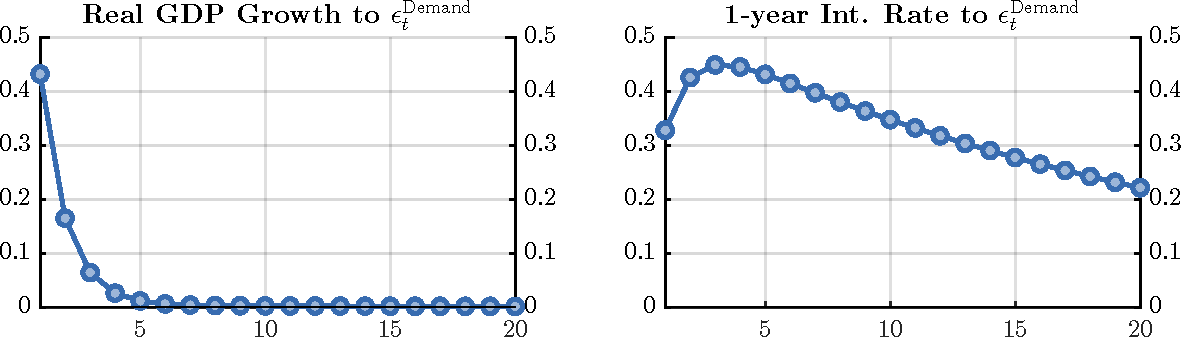
\includegraphics[width=.9\textwidth]{iv_sign}
		\end{center}%
		\vspace{0.2cm}
		\caption{\scshape{Impulse Responses to a Demand Shock}}
		\vspace{0.2cm}
		\scriptsize{{\scshape Note.} Median impulse responses of the log-difference of US real GDP and the 1-year Treasury bill yield to an expansionary demand shock across 1000 accepted draws. Identification: the monetary policy shock is pinned down via an external instrument (proxy SVAR); sign restrictions are then applied to identify the demand shock (GDP$>0$ and the 1-year rate $>0$ on impact), conditional on the IV-identified monetary policy impact. Bivariate VAR(1) estimated on quarterly US data, 1989:Q1--2019:Q4. Horizon: 20 quarters. Percentage points.}
		\label{fig:ivsign}
	\end{minipage}
\end{figure}

\subsection{Identification with Exogenous Variables}\label{sec:exog}

In some applications, the researcher observes a series $s_t$ that can be treated as contemporaneously exogenous to the VAR system --- an observed measure of the structural shock of interest, distinct from the latent shock vector $\varepsilon_t$. Rather than using $s_t$ as an external instrument in a two-stage IV regression (as in the proxy SVAR approach of Section~\ref{sec:iv}), one can include it directly as a contemporaneous regressor in each equation of the VAR:
\begin{equation}\label{eq:exog_var}
    x_t = c + \sum_{j=1}^{p}\Phi_j x_{t-j} + \delta s_t + u_t,
\end{equation}
where $\delta$ is a $k\times 1$ vector of impact coefficients. Because $s_t$ is exogenous, the OLS estimate $\hat{\delta}$ admits a direct structural reading: it is the on-impact response of each endogenous variable to a one-unit movement in $s_t$, with the other shocks held fixed. This is exactly the object that a column of the structural impact matrix $B$ records --- the contemporaneous effect of a single structural shock on the system (see Section~\ref{sec:struct_var}). This lets us read $\hat{\delta}$ as the first column of $B$, up to a choice of shock size: a one-unit change in $s_t$ gives the column as $\hat{\delta}$, while a one-standard-deviation change gives $\hat{\delta}\,\hat{\sigma}_s$, with $\hat{\sigma}_s$ the sample standard deviation of $s_t$.

Note that this approach is closely related to the proxy SVAR: both exploit the same external series to identify one structural shock, and they differ only in how that series enters. Here it enters directly as a contemporaneous regressor in the reduced-form VAR --- in the role of the shock $s_t$ --- whereas in the proxy SVAR of Section~\ref{sec:iv} the same series enters as an instrument $z_t$ in a two-stage IV regression. Under instrument exogeneity and a common lag structure, the two estimators are asymptotically equivalent~\citep{PlagborgMollerWolf2021}. The running example makes this concrete: the single \mci{mps} series is reused in both roles --- directly as the exogenous shock $s_t$ here, and as the instrument $z_t$ in the proxy SVAR of Section~\ref{sec:iv} --- which is harmless for illustration and is exactly the equivalence just stated.

\noindent\textbf{In MATLAB.} The exogenous-variable identification scheme is selected by setting \mc{VARopt\_exog.ident = 'exog'} and supplying $s_t$ via \mc{VARopt\_exog.exoshock}. A dedicated \mc{VARopt\_exog} struct (i.e.\ different from the \mc{VARoption} structure used throughout this section) keeps settings isolated from the rest of the examples. The identified responses are computed as: 

\begin{matlabcode}
% Set up and estimate
VARopt_exog = VARoption;
VARopt_exog.mnem      = Xmnem;
VARopt_exog.vnames    = Xvnames;
VARopt_exog.nsteps    = 20;
VARopt_exog.ident     = 'exog';
VARopt_exog.exoshock  = mps;
VARopt_exog.snames    = {bfeps('MonPol')};
VAR_exog = VARmodel(X, nlags, detc, VARopt_exog);
\end{matlabcode}

\noindent The \mc{VAR\_exog.B} field is populated with the estimated $B$ matrix, where the first column equals $\hat{\delta}\,\hat{\sigma}_s$: the OLS coefficient vector $\hat{\delta}$ from equation~\eqref{eq:exog_var}, scaled by $\hat{\sigma}_s$ (the sample standard deviation of $s_t$) to represent a one-standard-deviation shock. Storing this column in $B$ is a slight abuse of notation: the object recovered here is $\hat{\delta}$ (scaled), not a column of the structural impact matrix in the sense of the recursive or sign-restricted schemes. It is nonetheless convenient to place it in $B$, since the impact responses it generates are directly comparable across identification schemes.

As in the external-instrument case of Section~\ref{sec:iv}, the exogenous variable identifies a single structural shock, so only the first column of $B$ is identified; the remaining $k-1$ columns are set to zero because the other shocks are left unidentified.\footnote{Internally, \mc{VARmodel} completes $B$ to an invertible matrix in order to back out the structural shocks required by the historical decomposition; the unidentified columns are then zeroed in the stored \mc{VAR\_exog.B}, and their impulse responses, variance-decomposition shares, and historical-decomposition contributions are zeroed accordingly, since they carry no economic meaning.} Lags of $s_t$ can be included by setting \mc{VARopt\_exog.nlag\_exoshock} (default~0, contemporaneous only). General exogenous regressors not used for identification are passed via the fifth positional argument \mc{EXOG} of \mc{VARmodel}, separate from \mc{VARopt.exoshock}. For example, in a VAR for a small open economy, one may want to control for lags of world GDP; this can be done by passing a matrix of world GDP lags as \mc{EXOG}, so that the domestic block conditions on global conditions without treating foreign output as endogenous. 

Figure~\ref{fig:exog_ir} reports the impulse responses to the identified monetary policy shock, which can be obtained with the standard \mc{VARirplot} function (setting \mc{VARopt\_exog.pick=1}):

\vspace{0.2cm}
\begin{figure}[ht!]
	\centering%
	\begin{minipage}[b]{.9\textwidth}
		\begin{center}
			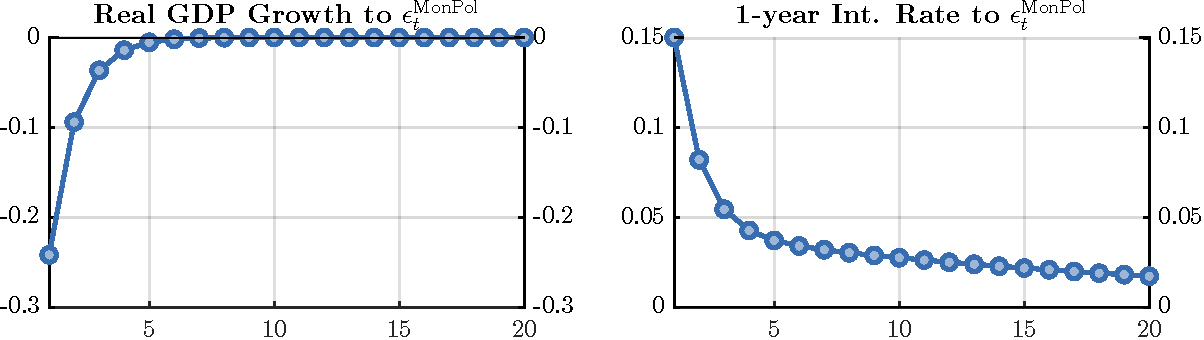
\includegraphics[width=.9\textwidth]{exog}
		\end{center}%
		\vspace{0.2cm}
		\caption{\scshape{Impulse Responses to a Monetary Policy Shock}}
		\vspace{0.2cm}
		\scriptsize{{\scshape Note.} Point estimates of the impulse responses of the log-difference of US real GDP and the 1-year Treasury bill yield to a contractionary monetary policy shock identified with an exogenous variable. The artificial exogenous variable \mci{mps} (see Box~\ref{box:mps}) enters as a contemporaneous regressor in each equation of the bivariate VAR; the first column of $B$ equals the OLS coefficient vector $\hat{\delta}$, scaled to a one-standard-deviation shock. Bivariate VAR(1) estimated on quarterly US data, 1989:Q1--2019:Q4. Horizon: 20 quarters. Percentage points.}
		\label{fig:exog_ir}
	\end{minipage}
\end{figure}

\subsection{Summary and Next Steps}

Section~\ref{sec:ident} has established seven approaches for recovering the structural impact matrix $B$ from the estimated reduced-form parameters. With an identified $B$ in hand, two tasks remain. Section~\ref{sec:inference} describes how to quantify uncertainty around structural impulse responses, variance decompositions, and historical decompositions. Section~\ref{sec:dynamic} then develops the three main tools for structural dynamic analysis: impulse response functions (Section~\ref{sec:irf}), forecast error variance decompositions (Section~\ref{sec:fevd}), and historical decompositions (Section~\ref{sec:hd}), together with their implementation in MATLAB. Statistical inference is covered before structural dynamic analysis because the figures and tables in Section~\ref{sec:dynamic} routinely display bootstrap confidence bands and Bayesian credible bands; the procedures introduced in Section~\ref{sec:inference} are therefore a prerequisite for that material.

\section{Statistical Inference}\label{sec:inference}

The figures produced in Section~\ref{sec:ident} display point estimates: impulse responses computed at the OLS parameter values $(\hat\Phi,\hat\Sigma_u)$, with no indication of sampling uncertainty. This section describes how the VAR Toolbox quantifies uncertainty around those point estimates.\footnote{Variance decompositions and historical decompositions, introduced in Section~\ref{sec:dynamic}, are affected by exactly the same sources of uncertainty and are treated analogously.}

How uncertainty is quantified depends on whether the identification scheme is \textit{point-identified} or \textit{set-identified}. Point-identified schemes --- Cholesky, long-run, exogenous-variable, and external-instrument identification --- uniquely determine the structural impact matrix $B$ from the reduced-form parameters $(\Phi,\Sigma_u)$. Uncertainty about structural objects therefore has a single source: \textit{parameter uncertainty}, the finite-sample variability in the estimated $(\hat\Phi,\hat\Sigma_u)$ that carries through to impulse responses, variance decompositions, and historical decompositions. Set-identified schemes --- sign restrictions, narrative sign restrictions, and their combination with external instruments --- admit many rotation matrices $Q$ at any fixed $(\Phi,\Sigma_u)$: even in large samples, the data do not select a unique $B$. These schemes face an additional source: \textit{identification uncertainty}, the irreducible non-uniqueness of the identified set that persists as $T\to\infty$ and cannot be reduced by collecting more data. The two sources are qualitatively different and call for qualitatively different inferential procedures.

By default, the toolbox accounts for parameter uncertainty; it can be switched off to return point estimates only. The field \mc{VARopt.inference} controls parameter uncertainty across all identification schemes. For point-identified models, parameter uncertainty is quantified via bootstrapping. For sign-restricted models, it is quantified via a Bayesian approach following \citet{Uhlig2005}; frequentist alternatives exist \citep[see e.g.][]{GranzieraMoonSchorfheide2018, GiacominiKitagawa2021} but are not implemented. When \mc{inference = 0}, no parameter uncertainty is incorporated: point-identified models return point estimates only, and sign-restricted models draw rotations at the OLS estimates $(\hat\Phi,\hat\Sigma_u)$, so the distribution of accepted draws reflects identification uncertainty alone. When \mc{inference = 1} (the default), parameter uncertainty is included: point-identified models compute bootstrap confidence bands, and sign-restricted models draw $(\Phi,\Sigma_u)$ from their posterior before drawing rotations, so the resulting distribution reflects both sources of uncertainty jointly.

\subsection{Bootstrap Inference (Point-Identified Models)} 

For short-run, long-run, exogenous-variable, and external-instrument identification, the structural impact matrix $B$ is uniquely determined by the reduced-form parameters. Setting \mc{VARopt.inference = 1} activates bootstrapping; all computations are performed internally by \mc{VARmodel}. Two variants are available, controlled by \mc{VARopt.method}:
\begin{itemize}
    \item \underline{\textit{Residual bootstrap}} (\mc{'bs'}): at each draw, a new artificial sample is constructed by resampling the estimated residuals \textit{with replacement} and feeding them through the estimated VAR, starting from the actual initial observations $x_1, \ldots, x_p$. This preserves the autocorrelation structure of the data but assumes the residuals are identically distributed over time.
    \item \underline{\textit{Wild bootstrap}} (\mc{'wild'}): each residual is multiplied by an independent Rademacher variable ($+1$ or $-1$ with equal probability). This relaxes the homoskedasticity assumption and is the preferred choice when residuals display time-varying variance.
\end{itemize}

\noindent For external instruments (\mc{VARopt.ident = 'iv'}), the wild bootstrap is the recommended default. Reduced-form VAR residuals in macroeconomic and financial data typically display conditional heteroskedasticity --- the residual variance varies over time, rising in volatile periods and falling in calm ones. The residual bootstrap assumes the residuals are identically distributed and therefore misrepresents this time variation; the wild bootstrap preserves the conditional variance at each date, delivering asymptotically valid inference under heteroskedasticity of unknown form. A further advantage in the proxy-SVAR setting is that reflecting each observation by $\pm 1$ preserves the time-series structure of the instrument --- including the zeros in subsamples where surprises are unavailable --- which resampling with replacement would scramble. The field \mc{VARopt.ndraws} controls the number of bootstrap replications (default: 1000) and \mc{VARopt.pctg} sets the confidence level (default: 95).

No standalone example is introduced here.\footnote{Section~\ref{sec:dynamic} presents a worked example in which the sign-restriction model of Section~\ref{sec:sr} is re-estimated with \mci{VARopt.inference = 1}.} Setting \mc{VARopt.inference = 1} before calling \mc{VARmodel} is all that is required; the call and all other options remain unchanged.

\subsection{Bayesian Inference (Sign-Restricted Models)}

Sign-restricted VARs face both parameter uncertainty and identification uncertainty. The VAR Toolbox addresses them jointly via the Bayesian approach of \citet{Uhlig2005}. The prior over $(\Phi, \Sigma_u)$ is the conjugate Normal-Inverse-Wishart distribution, which yields a closed-form posterior of the same family. For each accepted draw $d = 1, \ldots, D$:
\begin{enumerate}
\item Draw $\Sigma_u^{(d)}$ from the marginal Inverse-Wishart posterior.
\item Conditional on $\Sigma_u^{(d)}$, draw $\Phi^{(d)}$ from the Normal conditional posterior; retain the draw only if the implied VAR is stable (all eigenvalues of the companion matrix strictly inside the unit circle).
\item Compute the Cholesky factor $P^{(d)}$ of $\Sigma_u^{(d)}$. Draw a random orthogonal matrix $Q_j$ from the Haar measure on the space of $k \times k$ orthogonal matrices, via the QR factorization of a $k \times k$ matrix with i.i.d.\ standard normal entries.
\item Form $B_j^{(d)} = P^{(d)} Q_j$ and check whether the implied impact responses satisfy all sign restrictions.
\item If yes, retain $(B_j^{(d)}, \Phi^{(d)})$. If no, discard and return to step~3.
\end{enumerate}

\noindent Steps 1--2 are executed only when \mc{VARopt.inference = 1}. As discussed in Section~\ref{sec:sr}, when inference is disabled via \mc{VARopt.inference = 0}, $(\Phi, \Sigma_u)$ are fixed at their OLS estimates and only steps 3--5 are executed, so the distribution of accepted draws reflects identification uncertainty alone. Each accepted draw is a joint draw from the posterior over the reduced-form parameters \textit{and} over the set of admissible rotations; the resulting credible bands reflect both sources of uncertainty.

The combined \mc{sign+iv} scheme is an exception: \mci{VAR\_ivsr.Bmed(:,1)} is always the OLS IV point estimate and is not updated at steps~1--2, regardless of the \mc{VARopt.inference} flag. The credible bands for the IV-identified shock therefore do not reflect parameter uncertainty. Embedding parameter uncertainty for the IV-identified shock requires integrating the instrument into the model likelihood directly, as in \citet{CaldaraHerbst2019}; this is a qualitatively different model class and is not currently supported by the VAR Toolbox.

\subsection{Output Fields and Naming Convention}

The uncertainty bands are stored in the output struct returned by \mc{VARmodel}, following a consistent naming convention. For impulse responses, the relevant fields are:
\begin{itemize}
    \item \mc{.IRall} --- full array of draws, indexed along the fourth dimension; size $(h \times k \times k \times D)$, where $h$ is the number of horizons, $k$ the number of variables, and $D$ the number of draws.
    \item \mc{.IRbar} --- pointwise \textit{mean} across the $D$ draws. This is the central-tendency field for \textit{point-identified} schemes.
    \item \mc{.IRmed} --- pointwise \textit{median} across the $D$ draws. This is the central-tendency field for \textit{set-identified} (sign-restricted) schemes.
    \item \mc{.IRfp} --- the Fry-Pagan median-target response (Section~\ref{sec:sr}, Box~\ref{box:fp}): the impulse response of the single accepted rotation whose impact matrix is closest to the pointwise-median impact matrix in Frobenius norm. Populated for sign-restricted schemes only.
    \item \mc{.IRinf}, \mc{.IRsup} --- lower and upper percentile bands at level \mc{VARopt.pctg}.
\end{itemize}

\noindent The point estimate of the central tendency thus follows a different convention across the two families: \mc{.IRbar} (the mean) for point-identified schemes and \mc{.IRmed} (the median), together with the Fry-Pagan draw \mc{.IRfp}, for sign-restricted schemes. The percentile bands \mc{.IRinf} and \mc{.IRsup} are constructed in the same way in both cases. Recall that for point-identified schemes these fields are populated only when \mc{VARopt.inference = 1} (the default); when \mc{VARopt.inference = 0}, only the point-estimate field \mc{.IR} is available. For sign-restricted models, \mc{VARmodel} always populates \mc{.IRall}, \mc{.IRmed}, \mc{.IRfp}, \mc{.IRinf}, and \mc{.IRsup}, since the rotation draws are themselves the source of uncertainty.\footnote{Variance decompositions and historical decompositions follow analogous conventions. For point-identified schemes with bootstrap inference, the central-tendency fields are \mci{.VDbar} (pointwise mean) and \mci{.HDbar} (a struct with a \mci{.shock} subfield and other components). For sign-restricted models, the central-tendency fields are \mci{.VDmed} (unchanged) and \mci{.HDmed} (now a struct with a \mci{.shock} subfield); the band fields \mci{.HDinf} and \mci{.HDsup} are likewise structs with \mci{.shock} and other subfields. The fields \mci{.VDall}, \mci{.VDinf}, \mci{.VDsup} are unchanged across both identification families. These objects are documented in Sections~\ref{sec:fevd} and~\ref{sec:hd} respectively, where they are formally defined.} Section~\ref{sec:dynamic} describes how the plotting functions \mc{VARirplot}, \mc{VARvdplot}, and \mc{VARhdplot} use these fields to display uncertainty bands alongside point estimates.
 
\section{Structural Dynamic Analysis}\label{sec:dynamic}

Section~\ref{sec:ident} has established how to identify the $B$ matrix that maps structural shocks $\varepsilon_t$ into the reduced-form innovations $u_t$ via $u_t = B\varepsilon_t$, using zero contemporaneous restrictions, zero long-run restrictions, sign restrictions, narrative sign restrictions, external instruments, identification with exogenous variables, or combinations thereof. Section~\ref{sec:inference} has introduced the bootstrap and Bayesian procedures for quantifying uncertainty around the resulting structural objects. With an identified $B$ matrix in hand, one can define the three main tools of structural dynamic analysis, each addressing a distinct question about the role of shocks in driving economic fluctuations:

\begin{enumerate}
    \item \underline{\textit{How do shocks propagate over time?}} \ When a structural shock hits the economy, how do the endogenous variables respond dynamically? This question is answered by \textit{impulse response functions} (computed informally in each identification subsection of Section~\ref{sec:ident}).

    \item \underline{\textit{How important are different shocks on average?}} \ What portion of the forecast error variance in our variables is attributable to each structural shock? This is quantified through \textit{forecast error variance decompositions}.

    \item \underline{\textit{What drove specific historical episodes?}} \ Looking back at the data, which structural shocks were responsible for pushing the economy away from its equilibrium at particular points in time? This is revealed by \textit{historical decompositions}.
\end{enumerate}

\noindent The three tools provide complementary perspectives on the role of structural shocks: impulse responses trace dynamic propagation, variance decompositions measure average importance, and historical decompositions attribute observed fluctuations to specific shocks. Together, they allow us to move beyond estimating a VAR to understanding the underlying economic forces that shape macroeconomic outcomes.

Sections~\ref{sec:irf}--\ref{sec:hd} develop the mechanics of each tool; each subsection closes with its MATLAB implementation and the corresponding output figures from the built-in plotting functions. For the MATLAB implementation, this section uses the sign-restriction identification of Section~\ref{sec:sr}. The only substantive change relative to that section is \mc{inference = 1}, which incorporates parameter uncertainty in the rotation draws and populates the \mc{IRinf}/\mc{IRsup}, \mc{VDinf}/\mc{VDsup}, and \mc{HDinf}/\mc{HDsup} fields of the output struct:

\begin{matlabcode}
% Reset options, enable inference and re-estimate
VARopt.ident     = 'sign';
VARopt.R         = [ 1, -1;  % Real GDP
                     1,  1]; % 1-year rate
VARopt.IV        = [];
VARopt.snames    = {bfeps('Demand'), bfeps('MonPol')};
VARopt.inference = 1;
VARopt.pick      = 0;
VARopt.firstdate = datesnum(1);
VARopt.frequency = 'q';
rng(4)
VAR_infer = VARmodel(X, nlags, detc, VARopt);
\end{matlabcode}

%------------------------------------------
\subsection{Impulse Response Functions}\label{sec:irf}

Impulse response functions (henceforth, $IR$) answer the following question: \textit{What is the response over time of each endogenous variable in the VAR to a one-time increase in one of the structural shocks, holding all other structural shocks at zero?} By isolating the impact of a single shock while keeping all else constant, impulse responses allow us to trace the causal effect of that shock on the economy. They capture both the \textit{impact response} (the response at horizon $h=0$) and the \textit{persistence} (how long it takes for the effect to dissipate).

For example, for a monetary policy shock that raises the policy rate unexpectedly, the impulse response function traces how much GDP falls, how long the effect persists, and how the 1-year Treasury rate responds over the adjustment period.

\noindent \textbf{\sffamily\underline{How to compute impulse response functions}.} \ To understand how to compute impulse responses, we return to the simple bivariate structural VAR(1):
\begin{equation}
\left[ 
\begin{array}{c}
y_{t} \\ 
r_{t}
\end{array}
\right] =
\begin{bmatrix}
\phi_{11} & \phi_{12} \\ 
\phi_{21} & \phi_{22}
\end{bmatrix}
\left[ 
\begin{array}{c}
y_{t-1} \\ 
r_{t-1}
\end{array}
\right] +
\begin{bmatrix}
b_{11} & b_{12} \\ 
b_{21} & b_{22}
\end{bmatrix}
\begin{bmatrix}
\varepsilon_{t}^{Demand} \\ 
\varepsilon_{t}^{MonPol}
\end{bmatrix}
\end{equation}
To compute the impulse response to a specific shock, we first define an \textit{impulse selection vector} $s$ that picks out which shock we want to study. This is a $(k \times 1)$ vector that takes the value 1 for the shock of interest and 0 for all others. For example, to study the demand shock (the first shock), we set:
\begin{equation*}
s = \left[ 
\begin{array}{c}
1 \\ 
0
\end{array}
\right]
\end{equation*}
The impulse response to $\varepsilon_t^{Demand}$ can then be computed using:
\begin{equation}
x_t = \Phi x_{t-1} + Bs
\end{equation}
This equation describes how the system evolves when we ``shock'' it at time $t=0$ by setting $\varepsilon_0^{Demand} = 1$ (while keeping $\varepsilon_0^{MonPol} = 0$; here $Bs$ is the impact of the unit demand shock, not a structural shock entering the system every period), and then allow the system to evolve, setting $\varepsilon_h = 0$ for all $h \geq 1$.

More specifically, the impulse response at different horizons can be computed recursively:
\begin{equation}
\left\{ 
\begin{array}{ll}
IR_0 = Bs & \quad \text{(impact response)} \\[6pt]
IR_h = \Phi \cdot IR_{h-1} & \quad \text{for } h = 1, 2, ..., H \text{ (dynamic responses)}
\end{array}
\right.
\label{eq:ir_recursion}
\end{equation}
Define $\Theta_h \equiv \Phi^h B$ (henceforth the \textit{impulse response matrix} at horizon $h$; also written $IR_h$ in the MATLAB output). The $(i,j)$ element $(\Theta_h)_{ij}$ gives the response of variable $i$ to shock $j$ at horizon $h$. This is stored in the MATLAB array \mc{IR}, with \mc{IR(h+1,i,j)} giving the response of variable $i$ to shock $j$ at horizon $h$ (MATLAB uses 1-based indexing, so horizon $h=0$ is stored in row~1).

\noindent \textbf{\sffamily\underline{Interpretation}.} \ The impact response to shock $j$ is the $j$-th column of $B$. The rate at which the response dissipates is governed by the eigenvalues of $\Phi$ (or of the companion matrix $\mathcal{F}$ for $p > 1$): a dominant eigenvalue close to one in modulus implies slow decay; one close to zero implies rapid return to baseline. For a demand shock (first column of $B$), the impact responses are:
\begin{equation*}
IR_0 = 
\begin{bmatrix}
b_{11} & b_{12} \\ 
b_{21} & b_{22}
\end{bmatrix}
\begin{bmatrix}
1 \\ 
0
\end{bmatrix}
=
\begin{bmatrix}
b_{11} \\ 
b_{21}
\end{bmatrix}
\end{equation*}
The response at horizon $h=1$ is then:
\begin{equation*}
IR_1 = \Phi \cdot IR_0 = 
\begin{bmatrix}
\phi_{11} & \phi_{12} \\ 
\phi_{21} & \phi_{22}
\end{bmatrix}
\begin{bmatrix}
b_{11} \\ 
b_{21}
\end{bmatrix}
=
\begin{bmatrix}
\phi_{11}b_{11} + \phi_{12}b_{21} \\ 
\phi_{21}b_{11} + \phi_{22}b_{21}
\end{bmatrix}
\end{equation*}
and similarly for all subsequent horizons.

\noindent\textbf{\sffamily\underline{In MATLAB}.} \ Once \mc{VARmodel} has been run, impulse responses are plotted with \mc{VARirplot}. The function takes the \mc{IRmed} array, a populated \mc{VARopt} structure, and optionally \mc{IRinf} and \mc{IRsup} for uncertainty bands. Two additional optional arguments, \mc{INF2} and \mc{SUP2}, add a second (inner) uncertainty band when both are supplied. Key options: \mc{VARopt.figname} sets the save path; \mc{VARopt.pick = 0} (default) produces one figure per shock; \mc{VARopt.pick = j} produces a single figure for shock $j$:

\begin{matlabcode}
% Impulse responses with bands (VARirplot)	
VARopt.figname = 'graphics/sign_IR';
VARirplot(VAR_infer.IRmed, VARopt, VAR_infer.IRinf, VAR_infer.IRsup);
\end{matlabcode}

\noindent Figure~\ref{fig:sign_ir} shows the output from the sign-restriction identification with identification and parameter uncertainty: the solid blue line shows the element-wise median impulse response (\mc{VAR\_infer.IRmed}), while the shaded area spans the 95\% credible bands.  

\vspace{0.2cm}
\begin{figure}[ht!]
    \centering%
    \begin{minipage}[b]{.9\textwidth}
        \begin{center}
			\small \scshape(A) Demand shock \\
			\vspace{0.2cm}
            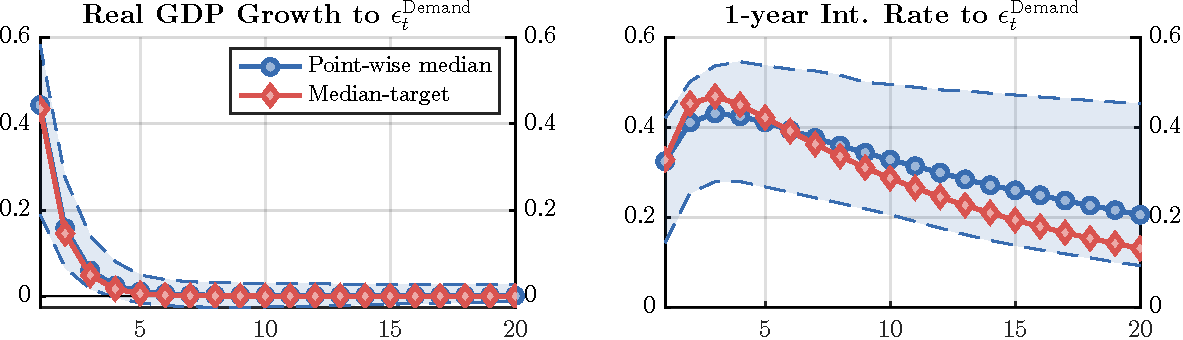
\includegraphics[width=.9\textwidth]{sign_IR_1}
            \\\vspace{0.4cm}
			(B) Monetary policy shock \\
			\vspace{0.2cm}
            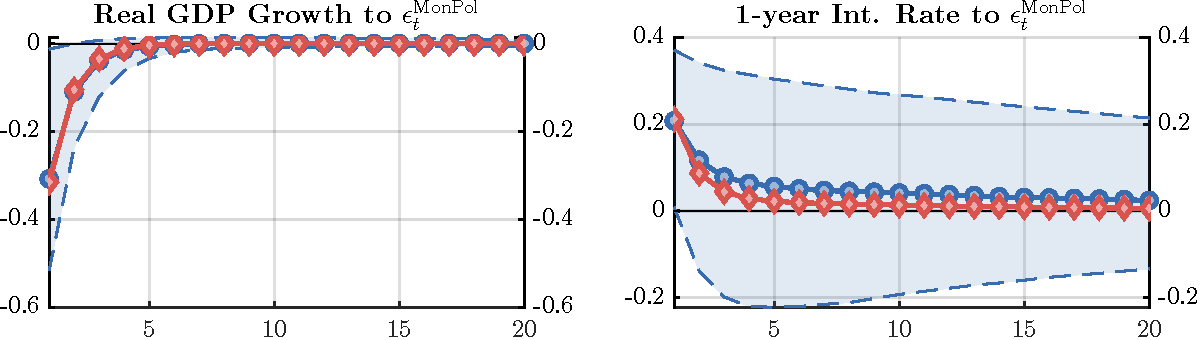
\includegraphics[width=.9\textwidth]{sign_IR_2}
        \end{center}
        \vspace{0.2cm}
        \caption{\scshape{Impulse Responses with Uncertainty Bands}}
        \vspace{0.2cm}
        \scriptsize{{\scshape Note.} Impulse responses of the log-difference of US real GDP and the 1-year Treasury bill yield to a demand shock (top panel) and a monetary policy shock (bottom panel), identified via sign restrictions. Blue line: element-wise median (\mci{VAR\_infer.IRmed}). Red line: Fry-Pagan median-target rotation (\mci{VAR\_infer.IRfp}). Shaded area: 95\% credible bands. Bivariate VAR(1) estimated on quarterly US data, 1989:Q1--2019:Q4. Horizon: 20 quarters. Percentage points.}
        \label{fig:sign_ir}
    \end{minipage}
\end{figure}

The figure reports one additional line beyond those plotted by \mc{VARirplot}. The solid red line is the Fry-Pagan median-target rotation (\mc{VAR\_infer.IRfp}), the single accepted draw whose responses lie closest to the element-wise median (Box~\ref{box:fp}). The two summaries differ in general, but the gap is more visible here than in Figure~\ref{fig:sign}: that figure set \mc{VARopt.inference = 0}, whereas this one accounts for parameter uncertainty, which widens the dispersion across draws and separates the median-target rotation from the element-wise median (Box~\ref{box:fp} explains that this dispersion is not the fundamental source of the gap, only what makes it larger here). Note that the red line is not produced by \mc{VARirplot} but superimposed separately --- see the Primer for the corresponding code.

\begin{notebox}
\boxentry{Growth-rate IRFs versus level IRFs}
\textbf{Growth-rate IRFs versus level IRFs.} \ The VAR Toolbox computes impulse responses for the variables as they enter the VAR --- in our running example, the \textit{log-difference} of US real GDP, i.e.\ the quarterly growth rate. The impulse response $IR_h^y$ measures how many percentage points the growth rate deviates from baseline $h$ periods after the shock.

This is often not the object of interest. When the question concerns the \textit{level} of output --- e.g.\ ``a monetary easing raises the level of GDP by $x\%$'' --- the relevant object is the \textit{cumulative impulse response}:
\begin{equation*}
\sum_{i=0}^{h} IR_i^y.
\end{equation*}
This follows directly from the Wold representation: since $y_t = \Delta \log Y_t$, the log-level $\log Y_{t+h}$ deviates from baseline by $\sum_{i=0}^{h} IR_i^y$.

Two consequences deserve attention. First, the zero long-run restriction of Section~\ref{sec:long} (monetary neutrality) is a restriction on $\sum_{i=0}^{\infty} IR_i^y = 0$, not on any individual growth-rate response. The condition $c_{12}=0$ --- the $(1,2)$ element of the long-run matrix $C = (I-\Phi)^{-1}B$ in \eqref{eq:long4} --- translates exactly to this cumulative sum being zero. Second, Figures~\ref{fig:long} and~\ref{fig:longCum} illustrate the difference directly: Figure~\ref{fig:long} plots the growth-rate responses, while Figure~\ref{fig:longCum} plots the cumulative (level) responses (which converge to zero by construction under neutrality).
\end{notebox}

%------------------------------------------
\subsection{Forecast Error Variance Decomposition}\label{sec:fevd}

Forecast error variance decompositions (henceforth, $VD$) answer the following question: \textit{What portion of the forecast error variance in each variable (at horizon $h$) is attributable to each structural shock?} While impulse responses tell us \textit{how} variables respond to shocks, variance decompositions tell us how \textit{important} each shock is in driving fluctuations in the variables of interest. This provides a different perspective: rather than tracing out the path of a single shock, we ask what fraction of the overall uncertainty about future values of our variables can be attributed to each structural shock.

For example, suppose we find that demand shocks explain 90\% of the forecast error variance in GDP at the 4-quarter horizon, while monetary policy shocks explain only 10\%. This tells us that, on average over the sample, demand shocks are the dominant source of GDP fluctuations, at least in the short run.

\noindent \textbf{\sffamily\underline{How to compute forecast error variance decompositions}.} \ To understand variance decompositions, we first need to define what we mean by a forecast error. The $h$-step-ahead forecast error is the difference between the actual value of the variable at time $t+h$ and what we would have predicted for that value based on information available at time $t-1$:\footnote{This handbook conditions on $\mathcal{F}_{t-1}$, so the $h$-step-ahead forecast error spans $h+1$ new shocks ($\varepsilon_t, \ldots, \varepsilon_{t+h}$). Some texts condition on $\mathcal{F}_t$, in which case the $h$-step error spans only $h$ new shocks.}
\begin{equation}
FE_{t+h} = x_{t+h} - \mathbb{E}_{t-1}[x_{t+h}]
\end{equation}

For a VAR(1), we can write the forecast error at different horizons as (note that under $\mathbb{E}_{t-1}$ conditioning, the $h$-step error accumulates $h+1$ new shocks):
\begin{align*}
FE_{t} &= x_t - \mathbb{E}_{t-1}[x_t] = B\varepsilon_t \\
FE_{t+1} &= x_{t+1} - \mathbb{E}_{t-1}[x_{t+1}] = \Phi B\varepsilon_t + B\varepsilon_{t+1} \\
FE_{t+2} &= x_{t+2} - \mathbb{E}_{t-1}[x_{t+2}] = \Phi^2 B\varepsilon_t + \Phi B\varepsilon_{t+1} + B\varepsilon_{t+2}
\end{align*}
In general, the $h$-step-ahead forecast error is:
\begin{equation}
FE_{t+h} = \sum_{i=0}^{h} \Phi^{h-i} B \varepsilon_{t+i}
\label{eq:forecast_error}
\end{equation}
Now consider the variance of the forecast error. Consider the case $h=0$. Under the $\mathbb{E}_{t-1}$ convention, the forecast error is $FE_t = B\varepsilon_t$, corresponding to the 1-step-ahead error and capturing the contemporaneous impact of shocks on the endogenous variables. Since the structural shocks are orthogonal and have unit variance, the variance of the forecast error for each variable is:
\begin{align*}
\text{Var}(y_t - \mathbb{E}_{t-1}[y_t]) &= b_{11}^2 + b_{12}^2 \\
\text{Var}(r_t - \mathbb{E}_{t-1}[r_t]) &= b_{21}^2 + b_{22}^2
\end{align*}
The forecast error variance decomposition for variable $y$ at horizon $h=0$ is then:
\begin{align*}
VD_y^{\varepsilon^{Demand}} &= \frac{b_{11}^2}{b_{11}^2 + b_{12}^2} \\[6pt]
VD_y^{\varepsilon^{MonPol}} &= \frac{b_{12}^2}{b_{11}^2 + b_{12}^2}
\end{align*}
Note that these decompositions sum to 1 for each variable --- this is by construction, since the structural shocks are the only sources of variation in the forecast error.

For longer horizons $h > 0$, the same logic applies, but we need to account for the cumulative effect of shocks from the present through horizon $h$. Let $\Theta_i = \Phi^i B$ denote the impulse response matrix at horizon $i$, as in Section~\ref{sec:irf}. Then the variance decomposition at horizon $h$ is:
\begin{equation}
VD_{y,h}^{\varepsilon^{j}} = \frac{\sum_{i=0}^{h} (\theta_{1j}^i)^2}{\sum_{i=0}^{h} \sum_{m=1}^{k} (\theta_{1m}^i)^2}
\label{eq:vd_formula}
\end{equation}
where $\theta_{1j}^i$ is the $(1,j)$ element of $\Theta_i$ (the response of variable $y$ to shock $j$ at horizon $i$). For a VAR($p$) with $p > 1$, replace $\Theta_i = \Phi^i B$ with the companion-form equivalent (see Box~\ref{box:companion}); the VAR Toolbox handles this substitution internally.

\noindent \textbf{\sffamily\underline{Interpretation}.} \ Unlike impulse responses, which trace out the effect of a single shock over time, variance decompositions aggregate across all possible shock realizations to give us an average measure of importance.

\noindent\textbf{\sffamily\underline{In MATLAB}.} \ \mc{VARvdplot} operates in two distinct modes depending on the arguments supplied. The array \mc{VD} has dimension $(H \times k \times k)$, where element \mc{VD(h,j,i)} is the FEVD share of shock $j$ for variable $i$ at horizon $h$ (1-indexed, matching the \mc{IR} array convention). The first mode requires only the \mc{VD} array and \mc{VARopt}. With \mc{VARopt.pick = 0} (the default), it produces a single figure with stacked area panels --- one panel per variable --- where each panel shows the FEVD shares of all shocks simultaneously; shares sum to one at every horizon. Setting \mc{VARopt.pick = j} ($j \geq 1$) restricts the output to variable $j$ only:

\begin{matlabcode}
% Variance decomposition — stacked area (VARvdplot)
VARopt.figname = 'graphics/sign_VD';
VARvdplot(VAR_infer.VDmed, VARopt);
\end{matlabcode}

\noindent Figure~\ref{fig:sign_vd} shows the stacked area FEVD from the sign-restriction identification of Section~\ref{sec:sr}. The code passes the element-wise median (\mc{VAR\_infer.VDmed}) to \mc{VARvdplot}; passing the Fry-Pagan draw (\mc{VAR\_infer.VDfp}) instead is equally valid --- the function accepts either. The trade-off is described in Box~\ref{box:fp}: element-wise median VD shares need not sum to one at every horizon, while Fry-Pagan shares do by construction. While convenient as they show the relative importance of all shocks simultaneously, stacked area charts do not display uncertainty bands. The second mode of \mc{VARvdplot}, described below, addresses this by plotting the FEVD share of a single shock with uncertainty bands, as described next.

\vspace{0.2cm}
\begin{figure}[ht!]
    \centering%
    \begin{minipage}[b]{.9\textwidth}
        \begin{center}
            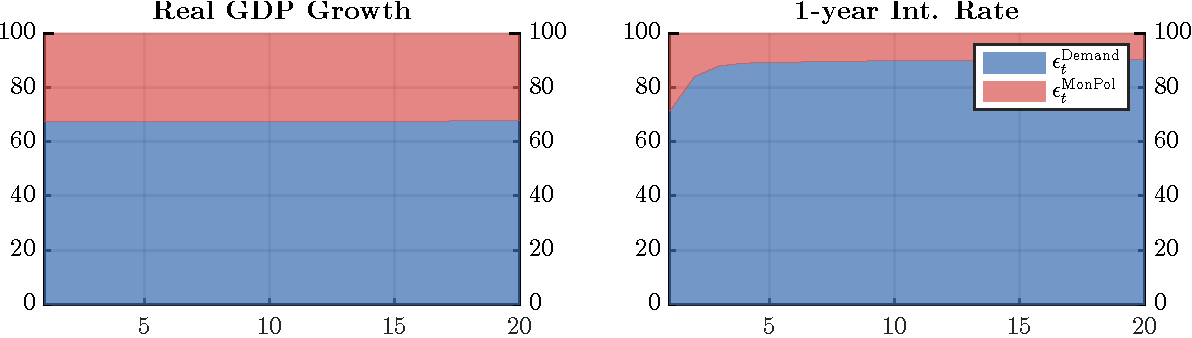
\includegraphics[width=.9\textwidth]{sign_VD}
        \end{center}
        \vspace{0.2cm}
        \caption{\scshape{Forecast Error Variance Decomposition (Stacked Area)}}
        \vspace{0.2cm}
        \scriptsize{{\scshape Note.} Stacked area forecast error variance decomposition from the sign-restricted bivariate VAR(1). Each panel shows the fraction of $h$-step-ahead forecast error variance attributable to each shock, computed from the element-wise median (\mci{VAR\_infer.VDmed}). Shares need not sum exactly to one at every horizon. Quarterly US data, 1989:Q1--2019:Q4. Horizon: 20 quarters.}
        \label{fig:sign_vd}
    \end{minipage}
\end{figure}

The second mode is activated by supplying \mc{VDinf} and \mc{VDsup} as additional arguments. In band mode, \mc{VARopt.pick} indexes \emph{shocks} (not variables): \mc{VARopt.pick = 0} produces one figure per shock; \mc{VARopt.pick = j} ($j \geq 1$) restricts to shock $j$ only. Each figure has one panel per variable, showing the forecast error variance decomposition share of the selected shock with uncertainty bands. A color can optionally be set via \mc{VARopt.color}; if unset, the function defaults to \mc{pantone('Blue')}. If \mc{VARopt} is reused for subsequent calls with different settings, reset \mc{pick} and \mc{color} to their defaults afterward:

\begin{matlabcode}
% Variance decomposition — with error bands (VARvdplot)
VARopt.figname = 'graphics/sign_VD_bands';
VARopt.pick    = 2;
VARopt.color   = pantone('Tomato');
VARvdplot(VAR_infer.VDmed, VARopt, VAR_infer.VDinf, VAR_infer.VDsup);
VARopt.pick    = 0;
VARopt.color   = [];
\end{matlabcode}

\noindent Figure~\ref{fig:sign_vd_bands} shows the band chart for the monetary policy shock. The wide credible bands reflect the identification uncertainty inherent in sign-restricted inference.

\vspace{0.2cm}
\begin{figure}[ht!]
    \centering%
    \begin{minipage}[b]{.9\textwidth}
        \begin{center}
            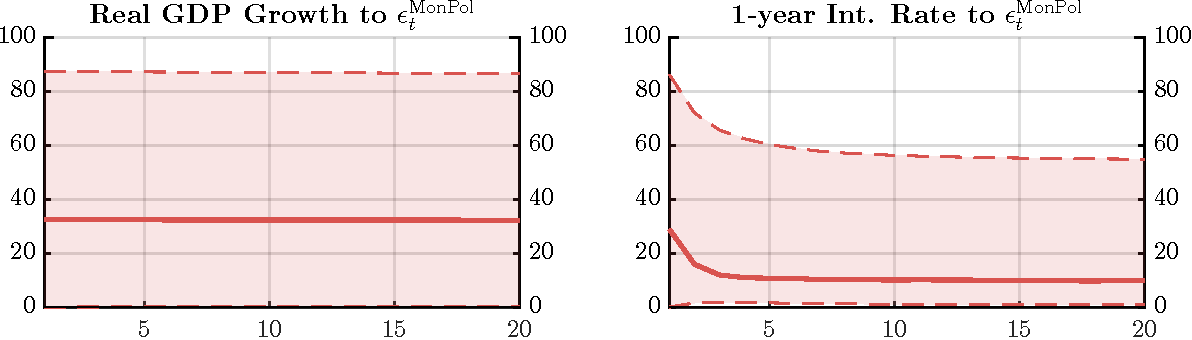
\includegraphics[width=.9\textwidth]{sign_VD_bands}
        \end{center}
        \vspace{0.2cm}
        \caption{\scshape{Forecast Error Variance Decomposition (Bands)}}
        \vspace{0.2cm}
        \scriptsize{{\scshape Note.} Fraction of forecast error variance attributable to the monetary policy shock with 68\% credible bands, from the sign-restricted bivariate VAR(1). Quarterly US data, 1989:Q1--2019:Q4. Horizon: 20 quarters.}
        \label{fig:sign_vd_bands}
    \end{minipage}
\end{figure}

\begin{notebox}
\boxentry{Three properties of the variance decomposition}
\textbf{Three properties of the variance decomposition.} Variance decompositions have several important properties that are worth highlighting:

\noindent \textit{\underline{1. The adding-up property}.} For any variable and any horizon $h$, the shares across all $k$ structural shocks sum to one:
\begin{equation*}
\sum_{j=1}^{k} VD_{y,h}^{\varepsilon^j} = 1.
\end{equation*}
This follows immediately from \eqref{eq:vd_formula}: the denominator equals the total forecast error variance, and the numerators partition it exactly because the structural shocks are orthonormal and span the full space of reduced-form innovations --- provided $B$ is square and invertible (full identification). Under partial identification, where not all shocks are identified, the shares need not sum to one.

\noindent \textit{\underline{2. The long-run limit}.} For a covariance-stationary VAR, as $h \to \infty$, the FEVD converges to the unconditional variance shares --- the fraction of the long-run variance of each variable attributable to each shock. These limiting shares depend on both the VAR dynamics $\Phi$ and the impact matrix $B$.

\noindent \textit{\underline{3. FEVD inherits identification}.} The shares are computed from $\Theta_i = \Phi^i B$, so they depend on the identifying assumptions through $B$. Two identification schemes that agree on one column of $B$ --- i.e.\ that identify the same shock in the same way --- will in general disagree on the variance shares, because the decomposition of residual variance among the remaining shocks depends on the full $B$ matrix. This contrasts with impulse responses: to characterize the dynamic effects of a single shock $j$, one column of $B$ suffices. The FEVD share of shock $j$, however, requires the full $B$ because the denominator aggregates the forecast error variance across all $k$ shocks.
\end{notebox}

%------------------------------------------
\subsection{Historical Decomposition}\label{sec:hd}

Historical decompositions (henceforth, $HD$) answer the following question: \textit{At each point in time, what is the contribution of each structural shock (past and present) to the deviation of each variable from its equilibrium?} While impulse responses describe hypothetical scenarios (``what if a shock hits?'') and variance decompositions provide average measures of importance, historical decompositions attribute observed fluctuations, period by period, to specific structural shocks.

For example, suppose GDP fell sharply in 2008:Q4. A historical decomposition would attribute that shortfall to the cumulative contributions of all past structural shocks --- demand and monetary policy shocks --- each weighted by its propagation through the VAR dynamics up to that date. The decomposition thus explains where GDP stands at any point in time as the sum of contributions from the entire history of shocks, not merely those that arrived in the current period. This provides a narrative of what drove the economy during that episode.

\noindent \textbf{\sffamily\underline{How to compute historical decompositions}.} \ To understand historical decompositions, recall the moving-average representation of the VAR (Section~\ref{sec:wold}), now written in finite-horizon form with the constant contribution and initial condition shown explicitly:
\begin{equation}
x_t = \sum_{s=0}^{t-1}\Phi^{s}c + \Phi^t x_0 + \sum_{s=0}^{t-1} \Phi^s B \varepsilon_{t-s}
\label{eq:wold_hd}
\end{equation}
For a VAR($p$) with $p > 1$, replace $\Phi$ and $B$ in \eqref{eq:wold_hd} with the companion matrix $\mathcal{F}$ and the expanded impact matrix $\mathcal{B}$ (see Box~\ref{box:companion}), retaining only the first $k$ rows of the resulting decomposition. The first term, $\sum_{s=0}^{t-1}\Phi^{s}c$, captures the cumulative contribution of the constant; the second term, $\Phi^t x_0$, captures the effect of the initial condition; and the third term is the cumulative contribution of all structural shocks from the initial period through period $t$, running backwards from the most recent shock $\varepsilon_t$ (at lag~0) to the oldest shock $\varepsilon_1$ (at lag~$t-1$).

For concreteness, consider $t=2$ in our simple bivariate VAR:
\begin{equation*}
x_2 = \underbrace{(I+\Phi)c}_{\text{Constant}} + \underbrace{\Phi^2 x_0}_{\text{Initial condition}} + \underbrace{B}_{=\Theta_0} \varepsilon_2 + \underbrace{\Phi B}_{=\Theta_1} \varepsilon_1
\end{equation*}
Writing this out in matrix form:
\begin{equation*}
\begin{bmatrix}
y_2 \\
r_2
\end{bmatrix}
=
\begin{bmatrix}
\text{const}_y \\
\text{const}_r
\end{bmatrix}
+
\begin{bmatrix}
\text{init}_y \\
\text{init}_r
\end{bmatrix}
+
\begin{bmatrix}
\theta_{11}^1 & \theta_{12}^1 \\
\theta_{21}^1 & \theta_{22}^1
\end{bmatrix}
\begin{bmatrix}
\varepsilon_1^{Demand} \\
\varepsilon_1^{MonPol}
\end{bmatrix}
+
\begin{bmatrix}
\theta_{11}^0 & \theta_{12}^0 \\
\theta_{21}^0 & \theta_{22}^0
\end{bmatrix}
\begin{bmatrix}
\varepsilon_2^{Demand} \\
\varepsilon_2^{MonPol}
\end{bmatrix}
\end{equation*}
For variable $y$, this becomes:
\begin{equation*}
y_2 = \text{const}_y + \text{init}_y + \theta_{11}^1 \varepsilon_1^{Demand} + \theta_{12}^1 \varepsilon_1^{MonPol} + \theta_{11}^0 \varepsilon_2^{Demand} + \theta_{12}^0 \varepsilon_2^{MonPol}
\end{equation*} 
The historical decomposition groups the terms by shock:
\begin{align*}
HD_{y,2}^{\varepsilon^{Demand}} &= \theta_{11}^1 \varepsilon_1^{Demand} + \theta_{11}^0 \varepsilon_2^{Demand} \\
HD_{y,2}^{\varepsilon^{MonPol}} &= \theta_{12}^1 \varepsilon_1^{MonPol} + \theta_{12}^0 \varepsilon_2^{MonPol} \\
HD_{y,2}^{\text{init}}  &= \text{init}_y \\
HD_{y,2}^{\text{const}} &= \text{const}_y
\end{align*}
These four components sum to $y_2$. The interpretation is straightforward:
\begin{itemize}
    \item $HD_{y,2}^{\varepsilon^{Demand}}$ is the cumulative contribution of all past demand shocks (that haven't fully dissipated yet) to $y$. \medskip
    \item $HD_{y,2}^{\varepsilon^{MonPol}}$ is the cumulative contribution of all past monetary policy shocks (that haven't fully dissipated yet) to $y$. \medskip
    \item $HD_{y,2}^{\text{init}}$ captures the influence of the initial condition, which decays toward zero as $t$ grows, provided the VAR is stable. \medskip
    \item $HD_{y,2}^{\text{const}}$ captures the cumulative contribution of the constant. In a stable VAR (all eigenvalues of the companion matrix strictly inside the unit circle), this term converges to $\mu_y$, the $y$-th element of the equilibrium vector $\mu=(I-\Phi)^{-1}c$ defined in \eqref{eq:mu}, as $t\to\infty$: it traces the path from zero toward the value $(I-\Phi)^{-1}c$. When the variables are covariance stationary, this limit equals the unconditional mean of $y$ and acts as the long-run level around which the shock contributions fluctuate; when the data are non-stationary (e.g.\ integrated variables estimated in log-levels), $(I-\Phi)^{-1}c$ is mathematically well-defined but economically uninterpretable as an unconditional mean (see Box~\ref{box:hd_loglevels} below).
\end{itemize} 

\noindent \textbf{\sffamily\underline{Interpretation}.}\ At each date, the decomposition assigns observed movements in each variable to specific structural shocks --- for instance, whether a recession was driven by demand shocks or monetary policy shocks.

\begin{notebox}
\label{box:hd_loglevels}
\boxentry{Historical decomposition: log-levels versus log-differences}
\textbf{Historical decomposition: log-levels versus log-differences.} The economic content of the initial condition and constant components depends on whether the VAR is estimated in log-differences or log-levels.

\noindent\textit{Log-differences VAR.} If the variables are growth rates, both components have a clean interpretation. The constant contribution converges to the average growth rate --- a structurally meaningful, finite number that is stable across sample windows and carries a direct economic interpretation. The initial condition captures the deviation of the economy from its long-run average at the start of the sample. The pre-sample history that drove the economy to $x_0$ is unobserved and unidentified; this deviation is therefore treated as a residual initial state rather than attributed to any specific structural shock. It decays toward zero just as any shock contribution does, provided the VAR is stable.
 
\noindent\textit{Log-levels VAR.} If the variables include log-levels of trending series such as log GDP, neither component has an economic interpretation on its own. The constant converges to the sample mean of log GDP --- a number that grows with the trend and changes with the sample window. The initial condition starts at the log-level of GDP in the first observation, which for a growing economy lies below the sample mean.

Together, however, the two components capture the underlying stochastic trend. Since all VAR structural shocks are transitory (I(0) by the stability assumption), subtracting their I(0) contributions from the approximately I(1) log-level series leaves an approximately I(1) residual --- a Beveridge-Nelson-type argument. That residual is the init-plus-constant baseline. Within the sample its mechanics are visible: the initial condition decays from $x_0$ toward zero while the constant rises from zero toward the sample mean, and their sum traces an upward path from $x_0$ to the sample mean that closely resembles the stochastic trend of log GDP. This is a finite-sample phenomenon --- eigenvalues strictly below one imply eventual convergence of both terms --- but over typical macroeconomic sample lengths the convergence is slow enough that the sum tracks the stochastic trend closely. When reading a historical decomposition from a levels VAR, the init and constant components should be lumped together and read as the stochastic trend, not interpreted individually.

\noindent\textit{A special case: $c = 0$.} The constant contribution is identically zero when the VAR is estimated without an intercept ($c = 0$). In a log-differences VAR this is a valid specification on demeaned growth rates, since average growth is zero by construction and the init contribution captures the initial deviation, which decays. In a log-levels VAR estimated on trending data, setting $c = 0$ is inadvisable: without a constant, the init contribution alone must absorb the entire I(1) stochastic trend, the model's long-run forecast converges to zero (not the sample mean), and the estimated AR coefficients are pushed toward unit roots to compensate. The constant is necessary in any levels VAR applied to trending series.
\end{notebox} 

\noindent\textbf{\sffamily\underline{In MATLAB}.} \ \mc{VARhdplot} operates in two distinct modes depending on the arguments supplied. Unlike \mc{VARvdplot}, which takes a plain array, \mc{VARhdplot} takes a \mc{HD} struct; the shock contributions are stored in the \mc{HD.shock} field. In sign-restricted VARs, \mc{VAR\_infer.HDmed} holds the element-wise median historical decomposition: the \mc{.shock} field is the element-wise median of shock contributions across all accepted draws, while the deterministic components (\mc{.init}, \mc{.const}, etc.) are copied from the Fry-Pagan draw (see Box~\ref{box:fp}). The function also accepts \mc{VAR\_infer.HDfp} (the Fry-Pagan draw) as the \mc{HD} argument. The trade-off mirrors that for variance decompositions: element-wise median contributions need not exactly reproduce the observed series when stacked, while Fry-Pagan contributions do by construction; any visible gap between the stacked contributions and the reference line in the stacked area figure reflects this non-summability. The first mode requires only the \mc{HD} struct and \mc{VARopt}. With \mc{VARopt.pick = 0} (the default), the function produces a single stacked area figure with one panel per variable, decomposing the observed path into the cumulative contributions of each structural shock and the deterministic components (constant and initial condition):

\begin{matlabcode}
% Historical decomposition — stacked area (VARhdplot)
VARopt.pick    = 0; % default: all shocks, stacked area
VARopt.figname = 'graphics/sign_HD';
VARhdplot(VAR_infer.HDmed, VARopt);
\end{matlabcode}

\noindent Figure~\ref{fig:sign_hd} shows the stacked area decomposition from the sign-restriction identification of Section~\ref{sec:sr}.

\vspace{0.2cm}
\begin{figure}[ht!]
    \centering%
    \begin{minipage}[b]{.9\textwidth}
        \begin{center}
            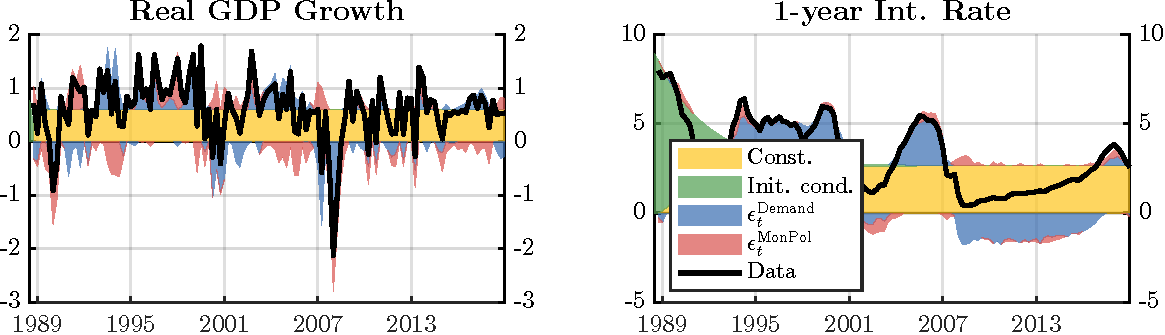
\includegraphics[width=.9\textwidth]{sign_HD}
        \end{center}
        \vspace{0.2cm}
        \caption{\scshape{Historical Decomposition (Stacked Area)}}
        \vspace{0.2cm}
        \scriptsize{{\scshape Note.} Stacked area historical decomposition from the sign-restricted bivariate VAR(1). Top panel: real GDP growth; bottom panel: 1-year Treasury bill rate. Each panel decomposes the observed path into the contributions of the demand shock, the monetary policy shock, and the deterministic components (constant and initial conditions). Shock contributions are element-wise medians across accepted draws (\mci{VAR\_infer.HDmed}) and need not exactly reproduce the observed series. Quarterly US data, 1989:Q1--2019:Q4. Percentage points.}
        \label{fig:sign_hd}
    \end{minipage}
\end{figure}

The second mode is activated by supplying \mc{HDinf} and \mc{HDsup} as additional arguments. In band mode, \mc{VARopt.pick} indexes \emph{shocks} (not variables): \mc{VARopt.pick = 0} produces one figure per shock; \mc{VARopt.pick = j} ($j \geq 1$) restricts to shock $j$ only. Each figure has one panel per variable, showing the time-varying contribution of shock $j$ with uncertainty bands. A color can optionally be set via \mc{VARopt.color}; if unset, the function defaults to \mc{pantone('Blue')}. If \mc{VARopt} is reused for subsequent calls with different settings, reset \mc{pick} and \mc{color} to their defaults afterward:

\begin{matlabcode}
% Historical decomposition — with error bands (VARhdplot)
VARopt.figname = 'graphics/sign_HD_bands';
VARopt.pick    = 2;
VARopt.color   = pantone('Tomato');
VARhdplot(VAR_infer.HDmed, VARopt, VAR_infer.HDinf, VAR_infer.HDsup);
\end{matlabcode}

\noindent Figure~\ref{fig:sign_hd_bands} shows the band chart for the monetary policy shock. The impulse responses, variance decompositions, and historical decompositions developed in Sections~\ref{sec:irf}--\ref{sec:hd} rest on the assumption that the true data-generating process is well approximated by a finite-order VAR. When this assumption is in doubt --- for instance, when the true lag order is large relative to the number of lags included in the estimated VAR, or when the VAR is otherwise misspecified --- the VAR-based IRFs may be biased. Section~\ref{sec:lp} introduces local projections as a specification-robust alternative: rather than iterating the fitted model forward, LP estimates the response at each horizon $h$ by a direct regression, delivering consistent estimates under weaker assumptions at the cost of efficiency when the VAR is correctly specified.

\vspace{0.2cm}
\begin{figure}[ht!]
    \centering%
    \begin{minipage}[b]{.9\textwidth}
        \begin{center}
            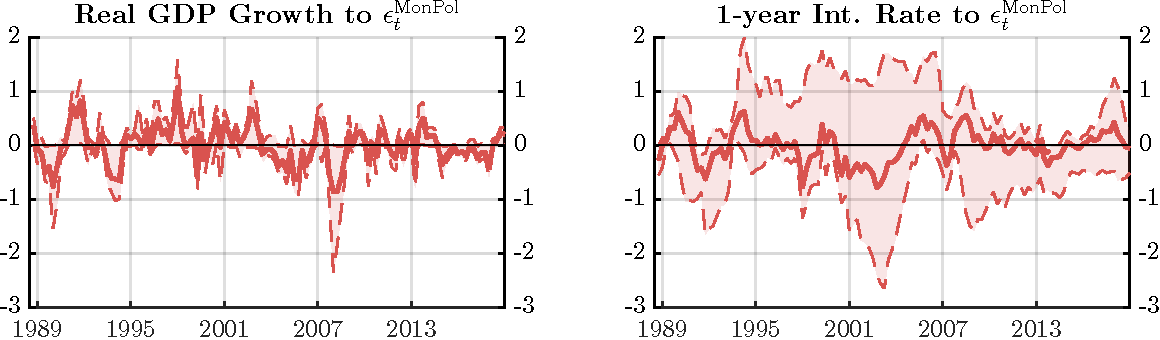
\includegraphics[width=.9\textwidth]{sign_HD_bands}
        \end{center}
        \vspace{0.2cm}
        \caption{\scshape{Historical Decomposition (Bands)}}
        \vspace{0.2cm}
        \scriptsize{{\scshape Note.} Time-varying contribution of the monetary policy shock to real GDP growth and the 1-year Treasury bill rate with 68\% credible bands, from the sign-restricted bivariate VAR(1). Quarterly US data, 1989:Q1--2019:Q4. Percentage points.}
        \label{fig:sign_hd_bands}
    \end{minipage}
\end{figure}

\section{Local Projections}\label{sec:lp}

Local projections (LP), introduced by \cite{Jorda2005}, estimate the impulse response at each horizon $h$ directly by regressing the $h$-step-ahead outcome on the shock of interest and lagged controls, without iterating a fully specified dynamic model forward. More broadly, local projections and VAR-based impulse responses are two implementations of the same object: under a common identification scheme and a common lag structure, both estimate the same population impulse response function, and the distinction is one of implementation. The VAR fits a fully specified dynamic model and iterates the fitted system forward to trace the response; LP estimates the response at each horizon by a separate, direct regression.

\subsection{A Brief Overview}\label{sec:lp_background}

A key premise of LP is that the researcher has access either to an identified shock series, used directly, or to an external instrument correlated with the shock of interest. The two cases give the two forms of the LP estimator: LP ordinary least squares (LP-OLS), which regresses directly on the shock series, denoted $s_t$; and LP two-stage least squares (LP-IV), which uses an external instrument, denoted $z_t$, to identify the effect of an endogenous treatment $d_t$. The two symbols follow the convention of the proxy-SVAR and exogenous-variable schemes of Sections~\ref{sec:iv} and~\ref{sec:exog}: $s_t$ for a series that enters the regression directly as the shock, $z_t$ for an instrument.
 
For a scalar outcome $x_{i,t}$ --- the $i$-th element of the endogenous vector $x_t$, i.e.\ one of the variables of the system --- and shock series $s_t$, the LP-OLS estimator runs:
\begin{equation}\label{eq:lp}
    x_{i,t+h} = \alpha_h + \beta_h s_t + \gamma_h' w_t + e_{t+h}, \qquad h = 0, 1, \ldots, H,
\end{equation}
where $i$ indexes the variables of the system $x_t$, $w_t$ is a vector of control variables --- typically the lagged values of the same variables that would enter a VAR specification --- and $e_{t+h}$ is the $h$-step-ahead forecast error. The projection is run separately for each outcome $i$, so the intercept, slope coefficients, and error carry an implicit $i$ subscript, suppressed throughout for readability. The sequence of estimated coefficients $\{\hat{\beta}_h\}_{h=0}^{H}$ directly traces the impulse response of $x_{i,t+h}$ to $s_t$. The outcome enters in whatever transformation the variable is supplied: when $x_{i,t}$ is a log-difference, $x_{i,t+h}$ is the growth rate $h$ periods ahead, so $\hat{\beta}_h$ traces the response of the growth rate, matching the VAR IRF convention of Section~\ref{sec:dynamic}. Confidence bands use Newey-West HAC standard errors with bandwidth $L = h-1$ at each horizon $h$.

When the structural shock cannot be measured directly but an external instrument $z_t$ is available, LP-IV replaces the regressor with the endogenous policy variable $d_t$, instrumented by $z_t$:
\begin{equation}\label{eq:lp_iv}
    x_{i,t+h} = \alpha_h + \beta_h d_t + \gamma_h' w_t + e_{t+h}, \qquad h = 0, 1, \ldots, H,
\end{equation}
where $d_t$ is instrumented by $z_t$ via horizon-by-horizon 2SLS. The coefficient $\hat{\beta}_h^{IV}$ estimates the causal effect of a change in $d_t$ (induced by $z_t$) on $x_{i,t+h}$, rather than the reduced-form effect of $z_t$ itself. The instrument must satisfy the same relevance and exogeneity conditions as in the proxy SVAR of Section~\ref{sec:iv}: $z_t$ must be correlated with $d_t$ and uncorrelated with the other structural shocks.

LP has two main attractions relative to VAR-based IRFs. First, it is \textit{robust to misspecification}: if the true data-generating process is not a finite-order VAR, the LP estimator still consistently estimates the impulse response at each horizon, provided the identifying variable ($s_t$ in LP-OLS, the instrument $z_t$ in LP-IV) is exogenous and $w_t$ is rich enough to absorb the predictable component of $x_{i,t+h}$. Second, the LP framework extends readily to nonlinear and state-dependent settings. The main cost is \textit{efficiency}: by fitting a separate regression at each horizon, LP does not exploit the cross-horizon parameter restrictions implied by the VAR dynamics, so LP estimates are less efficient when the VAR is correctly specified.\footnote{See \cite{PlagborgMollerWolf2021} for a formal treatment of the efficiency-robustness trade-off and a proof that LP and VAR-based estimators identify the same population impulse responses when the VAR is correctly specified and lag controls are sufficiently rich (formally, $p\to\infty$ as $T\to\infty$).}

A few practical caveats. LP estimates become noisier at long horizons because the forecast error $e_{t+h}$ grows in variance with $h$, so the trade-off between precision and horizon coverage should inform the choice of $H$. The bandwidth $L = h-1$ matches the MA order of the forecast error under a correctly specified VAR but may be conservative when the true MA order is shorter. Inference relies on asymptotic approximations; bootstrap procedures for LP are not currently implemented in the VAR Toolbox.

\subsection{Estimation and Identification}\label{sec:lp_estimation}

In the VAR Toolbox, local projections are implemented by the function \mc{LP = LPmodel(ENDO, TREAT, CTRL, nlag, const, LPopt, EXOG, nlag\_ex)}. There are five required inputs: (i) a matrix of outcomes, \mc{ENDO}; (ii) the shock or treatment series, \mc{TREAT}, common to all outcomes --- namely, the shock $s_t$ in LP-OLS, the endogenous treatment $d_t$ in LP-IV; (iii) a matrix of controls, \mc{CTRL}; (iv) an integer lag length, \mc{nlag}; and (v) the deterministic component, \mc{detc} (0 = none, 1 = constant, 2 = constant and trend). The controls are passed in contemporaneous form and lagged internally: \mc{LPmodel} enters only lags $1,\ldots,$\mc{nlag} of \mc{CTRL} as regressors --- never their contemporaneous values --- so the user does not lag the controls beforehand.\footnote{Unlike \mc{VARmodel}, lags of the outcome are not added automatically. Passing the full \mc{ENDO} matrix as \mc{CTRL} reproduces the VAR control set.} An optional sixth argument \mc{LPopt} holds all estimation, identification, and plotting options (created with \mc{LPoption}; a sensible default is used if omitted); optional seventh and eighth arguments \mc{EXOG} and \mc{nlag\_ex} accept exogenous regressors and their lag order. The estimator is univariate by construction --- each impulse response comes from a separate horizon-by-horizon regression of one outcome on the shock --- but when \mc{ENDO} has $N$ columns the same specification (identical shock, controls, lags, and options) is looped over them, returning the responses as $H \times N$ matrices in the manner of \mc{VARmodel}. A single column reproduces the classic univariate call.

As with \mc{VARopt}, \mc{LPopt} is the input side of the toolbox: a struct, created once with \mc{LPoption}, that carries estimation, identification, and plotting options across successive calls. Although optional, it is created in the example below so that variable mnemonics can be passed through \mc{LPopt.mnem}. The choice between the two LP estimators (OLS and IV) is governed by a single field: when \mc{LPopt.IV} is empty (the default), \mc{LPmodel} runs LP-OLS, projecting directly on \mc{TREAT}; when \mc{LPopt.IV} is set to an external instrument, it runs LP-IV, treating \mc{TREAT} as the endogenous variable instrumented by \mc{LPopt.IV} via horizon-by-horizon 2SLS. The two estimators are otherwise identical in call structure. The running example uses the same bivariate system as the preceding sections: GDP growth (\mc{dlngdp}) and the level of the 1-year Treasury rate (\mc{i1yr}), with the \mc{mps} series from Section~\ref{sec:iv} entering as the shock $s_t$ in LP-OLS and as the external instrument $z_t$ in LP-IV.

\noindent \textbf{\sffamily\underline{LP-OLS}.}\ Options are passed via \mc{LPopt} (from \mc{LPoption}); the shock normalization is set to one standard deviation (\mc{impact = 0}):

\begin{matlabcode}
% Set up LP-OLS options
LPopt          = LPoption;
LPopt.nsteps   = VARopt.nsteps; % match VAR horizon
LPopt.pctg     = 90;            % 90% confidence bands
LPopt.impact   = 0;             % 1-std-dev shock
LPopt.mnem     = Xmnem;         % mnemonics names 
LPopt.vnames   = Xvnames;       % labels for plots
\end{matlabcode}

\noindent Table~\ref{tab:lpopt} documents the fields of \mc{LPopt} that control estimation and plotting, grouped by role, together with their default values and meaning; the table follows \mc{LPoption.m}, which can be inspected directly for the same information. Of the fields in Table~\ref{tab:lpopt}, only \mc{longdiff} and \mc{nlag\_iv} are specific to local projections; every other field shares the name and meaning of the corresponding \mc{VARopt} field (Table~\ref{tab:varopt}), including the estimation fields \mc{nsteps}, \mc{pctg}, and \mc{impact} and the instrument field \mc{IV}. In particular, the figure-export and panel-appearance fields are common to both structures, and \mc{LPirplot} reads them as \mc{VARirplot} reads them from \mc{VARopt}, so the same plotting conventions apply.\bigskip

\begingroup
\footnotesize
\setlength{\defaultaddspace}{0.8em}
\renewcommand{\arraystretch}{0.9}
\renewcommand{\mc}[1]{\colorbox{script!80}{\texttt{#1}}}
\begin{longtable}{l@{\hspace{0.7em}}p{0.6\textwidth}}
\caption{Fields of the \mc{LPopt} options structure, with default values.}\label{tab:lpopt}\\\toprule
\textbf{Field (default)} & \textbf{Description}\\
\midrule
\endfirsthead
\multicolumn{2}{l}{\itshape Table~\ref{tab:lpopt}, continued}\\
\toprule
\textbf{Field (default)} & \textbf{Description}\\
\midrule
\endhead
\midrule
\multicolumn{2}{r}{\footnotesize\itshape continued on next page}\\
\endfoot
\bottomrule
\endlastfoot
\addlinespace
\multicolumn{2}{l}{\underline{\textit{Estimation}}}\\[2pt]
\mc{nsteps = 40}          & Number of horizons $H$ for the projection IRFs.\\
\mc{pctg = 95}            & Outer confidence level for error bands (percent).\\
\mc{impact = 0}           & Shock size: 0 = standardize the projection variable (the shock $s_t$ in LP-OLS, the treatment $d_t$ in LP-IV) to one standard deviation; 1 = leave it unchanged, so the response is per unit of that variable.\\
\mc{longdiff = 0}         & 1 = use the long-difference dependent variable $x_{i,t+h}-x_{i,t-1}$ instead of the level $x_{i,t+h}$.\\
\addlinespace
\multicolumn{2}{l}{\underline{\textit{IV identification}}}\\[2pt]
\mc{IV = []}              & External instrument for the endogenous treatment $d_t$ passed to \mc{LPmodel}; empty = LP-OLS. Mirrors the \mc{VARopt.IV} convention.\\
\mc{nlag\_iv = 0}         & Number of instrument lags added as extra instruments under LP-IV: 0 = just-identified (Wald estimator per horizon); $n>0$ adds lags $1,\ldots,n$ of \mc{IV} after FWL. Requires \mc{nlag\_iv}~$\leq$~\mc{nlag}.\\
\addlinespace
\multicolumn{2}{l}{\underline{\textit{Variable and shock labels}}}\\[2pt]
\mc{mnem = \{\}}          & Outcome mnemonics: valid MATLAB identifiers (no spaces or special characters) used to name the per-outcome sub-structs \mc{LP.(.)}. Falls back to \mc{vnames} if empty.\\
\mc{vnames = \{\}}        & Outcome display labels for plots and tables (may contain spaces or \LaTeX), one per column of the response matrix. Falls back to \mc{mnem} if empty.\\
\mc{snames = \{\}}        & Shock name (single entry for LP).\\
\addlinespace
\multicolumn{2}{l}{\underline{\textit{Figure export}}}\\[2pt]
\mc{figname = []}         & Prefix string for the exported figure filename.\\
\mc{figsize = []}         & Figure window size \mc{[width, height]} in cm.\\
\mc{quality = 2}          & Export quality: 2 = high via \mc{exportgraphics} (recommended, R2020a+), 1 = high via Ghostscript (legacy fallback), 0 = low via \mc{print -dpdf}.\\
\mc{suptitle = 0}         & 1 = add a super-title above the figure panels.\\
\addlinespace
\multicolumn{2}{l}{\underline{\textit{Panel appearance (used by \mc{LPirplot})}}}\\[2pt]
\mc{latex = 1}            & 1 = use the \LaTeX{} interpreter for figure text.\\
\mc{font = 'Helvetica'}   & Font name for figure text; \mc{''} = MATLAB default.\\
\mc{grid = 1}             & 1 = show gridlines.\\
\mc{marker = 'o'}         & Marker style for the IR line (\mc{'o'}, \mc{'none'}, etc.).\\
\mc{subplot = []}         & Subplot grid \mc{[rows cols]}; empty = auto from \mc{sqrt(nvars)}.\\
\mc{shorttitle = 0}       & 1 = show the variable name only as the panel title; 0 = `variable to shock'.\\
\mc{color = []}           & Line and band color (RGB triplet); empty = \mc{pantone('Blue')}.\\
\mc{linestyle = '-'}      & IR line style (\mc{'-'}, \mc{'--'}, \mc{':'}, \mc{'-.'}).\\
\mc{hstart = 1}           & First horizon label on the x-axis (0 or 1).\\
\mc{xlim = []}            & x-axis limits \mc{[lo hi]}; empty = auto from \mc{hstart:H}.\\
\mc{ylim = []}            & y-axis limits \mc{[lo hi]}; empty = auto.\\
\mc{xtick = []}           & x-tick positions; empty = auto.\\
\mc{xlabel = ''}          & x-axis label applied to each panel; empty = none.\\
\mc{ylabel = ''}          & y-axis label applied to each panel; empty = none.\\
\mc{dualaxis = 1}         & 1 = dual-axis panel style (tick marks mirrored on the left and right y-axes, box off, closure tick at the top); 0 = off.\\
\mc{visible = 1}          & 1 = show figure windows; 0 = suppress display (save only).\\
\end{longtable}
\endgroup

\noindent Passing the full matrix \mc{X} --- the two endogenous variables, GDP growth and the 1-year Treasury rate --- rather than a single column returns the full set of LP results --- impulse responses, confidence bands, and the per-horizon estimation output --- for all variables at once. In terms of equation~\eqref{eq:lp}: the first argument supplies $x_{i,t+h}$ (one column per outcome), \mc{mps} is the shock $s_t$, and the third argument provides the lag control vector $w_t$ (lags of GDP growth and the 1-year Treasury rate). To keep these roles explicit at the call site, the example aliases the first and third arguments as \mc{ENDO = X} (the outcomes) and \mc{CTRL = X} (the controls) before invoking \mc{LPmodel}. Here both equal \mc{X}, so the assignment is redundant; it serves only to mark the two slots as conceptually distinct and to show where a richer control set would enter --- through \mc{CTRL} alone:

\begin{matlabcode}
% Run LP-OLS for all endogenous variables in a single matrix call
ENDO = X;   % outcomes x_{i,t+h}
CTRL = X;   % controls w_t (lags constructed internally)
LP = LPmodel(ENDO, mps, CTRL, nlags, detc, LPopt);
\end{matlabcode}

\noindent At the impact horizon ($h=0$), equation~\eqref{eq:lp} reproduces a single reduced-form VAR equation augmented with the contemporaneous shock: GDP growth is regressed on a constant, the shock \mc{mps}, and lags of GDP growth and the 1-year Treasury rate. Given a common lag structure, this $h=0$ regression is exactly one equation of the exogenous-variable VAR of equation~\eqref{eq:exog_var} (Section~\ref{sec:exog}), in which the same shock $s_t$ enters every equation as a contemporaneous regressor: the two are the same OLS projection of GDP growth on the shock and the lag controls. The schemes differ only beyond impact. The exogenous-variable VAR estimates this contemporaneous system once and iterates the estimated coefficients forward to all horizons, so relative to LP --- which re-estimates a fresh regression at each horizon --- it involves exactly the same regression at impact and (weakly) fewer regressions overall, a trade-off examined in Section~\ref{sec:lp_exog}. The sequence $\{\hat{\beta}_h\}$ then traces how that same contemporaneous innovation propagates as the horizon $h$ grows, one direct regression at a time.

\noindent \textbf{\sffamily\underline{LP-IV}.}\ To identify the causal effect of the 1-year Treasury rate on output, LP-IV uses the same call with the level of the 1-year rate \mc{ENDO(:,2)} passed as \mc{TREAT} (the endogenous treatment $d_t$) and \mc{mps} supplied through \mc{LPopt.IV} (the external instrument $z_t$). The \mc{ENDO} and \mc{CTRL} aliases defined above carry over unchanged. This mirrors the proxy-SVAR of Section~\ref{sec:iv}, where \mc{VARopt.IV} likewise holds the external instrument:

\begin{matlabcode}
%  Set up and run LP-IV
LPopt_IV         = LPoption;
LPopt_IV.nsteps  = VARopt.nsteps;
LPopt_IV.pctg    = 90;
LPopt_IV.impact  = 0;
LPopt_IV.IV      = mps;   % external instrument
LPopt_IV.mnem    = Xmnem; % name per-variable sub-structs
LP_IV = LPmodel(ENDO, ENDO(:,2), CTRL, nlags, detc, LPopt_IV);
\end{matlabcode}

\noindent The function \mc{LPmodel.m} estimates each horizon's IV coefficient via the Frisch-Waugh-Lovell (FWL) theorem. Rather than placing the lag controls $w_t$ alongside the treatment in the 2SLS step, it first partials $w_t$ out of the outcome $x_{i,t+h}$, the treatment $d_t$, and the instrument $z_t$ --- regressing each on $w_t$ and retaining the residuals --- and then runs the first and second stages on the residualized series. By FWL, the coefficient on $d_t$ is numerically identical to the one obtained by including $w_t$ directly, so the per-horizon estimate matches a standard 2SLS routine. The first-stage F-statistic, stored per horizon in \mc{LP\_IV.dlngdp.hN.Fstat\_fs}, should exceed the conventional rule-of-thumb value of 10 (see the first-stage discussion in Section~\ref{sec:iv}) for the instrument to be considered relevant. With \mc{nlag\_iv}~$=0$ --- a single instrument for a single treatment, the just-identified case --- the estimator reduces to the Wald estimator at each horizon.

\noindent\textbf{\sffamily\underline{Structure of the \mc{LPmodel} output}.}\ The \mc{LPmodel} function returns a single structure \mc{LP} that collects all output from the local projection estimation. Its top-level fields are:

\begin{matlaboutput}
disp(LP)
	dlngdp: [1×1 struct]
	i1yr: [1×1 struct]
	eqnames: {2×1 cell}
	ENDO: [123×2 double]
	TREAT: [123×1 double]
	CTRL: [123×2 double]
	EXOG: []
	nlag: 1
	nlag_ex: 0
	const: 1
	ntotcoeff: 4
	IR: [20×2 double]
	INF: [20×2 double]
	SUP: [20×2 double]
\end{matlaboutput}

\noindent where the main elements are:

\begin{itemize}[noitemsep]
    \item \mc{dlngdp}, \mc{i1yr}: one sub-struct per variable, each the full univariate LP output for that column (its own $H \times 1$ \mc{IR}/\mc{INF}/\mc{SUP}, joint-test fields, and per-horizon sub-structs \mc{h1}, \ldots, \mc{hH}). The names come from \mc{LPopt.mnem} (set to \mc{\{'dlngdp','i1yr'\}} above); if \mc{mnem} is empty, or its entries are not valid unique field names (e.g.\ display labels with spaces), the sub-structs default to \mc{eq1}, \ldots, \mc{eqN}. The resolved names are also stored in \mc{LP.eqnames} (an $N\times1$ cell), mirroring \mc{VAR.eqnames}.
	\item \mc{ENDO}, \mc{TREAT}, \mc{CTRL}, \mc{EXOG}: input data echoed back for traceability.
    \item \mc{nlag}, \mc{const}: lag order and deterministic specification.
    \item \mc{IR}, \mc{INF}, \mc{SUP}: impulse responses and Newey-West confidence bands ($H \times N$); column $i$ is the response of variable $i$.
\end{itemize}

\noindent Each per-variable sub-struct is itself a complete univariate LP output: it holds that variable's own impulse responses (\mc{IR}/\mc{INF}/\mc{SUP}), the joint-test fields (\mc{jtest\_chi2}, \mc{jtest\_df}, \mc{jtest\_pval}), and one sub-struct per horizon (\mc{h1}, \ldots, \mc{h20}) storing the horizon-$h$ estimation results (OLS here; 2SLS under LP-IV). For example, the full output for the GDP growth equation (the first column of \mc{X}) is inspected with \mc{disp(LP.dlngdp)}:

\begin{matlaboutput}
>> disp(LP.dlngdp)
	ENDO: [123×1 double]
	TREAT: [123×1 double]
	CTRL: [123×2 double]
	EXOG: []
	nlag: 1
	nlag_ex: 0
	const: 1
	ntotcoeff: 4
	jtest_chi2: 62.8949
	jtest_df: 20
	jtest_pval: 2.5152e-06
	h1: [1×1 struct]
	h2: [1×1 struct]
	h3: [1×1 struct]
	.
	.
	.	
	h20: [1×1 struct]
	IR: [20×1 double]
	INF: [20×1 double]
	SUP: [20×1 double]
\end{matlaboutput}

\noindent\textbf{Normalization to 25 bps.}\ To compare the two methods on a common scale --- the response to a 25 basis point increase in the 1-year Treasury rate --- both sets of impulse responses are rescaled after estimation. For LP-OLS, the scale factor is the ratio of the target change (0.25 percentage points) to the impact response of the 1-year Treasury to a 1-standard-deviation \mc{mps} shock, \mc{LP\_IR(1,2)}. For LP-IV, the impulse responses are already expressed per one-standard-deviation move in the treatment (the \mc{impact = 0} normalization divides by the standard deviation of the 1-year rate); rescaling to a 25 basis point move therefore divides \mc{0.25} by \mc{std(X(:,2))}:

\begin{matlabcode}
ir_col      = 2;                        % column index of i1yr in X
scale_ols   = 0.25 / LP_IR(1,ir_col);   % LP-OLS normalization
scale_iv    = 0.25 / std(X(:,ir_col));  % LP-IV normalization
LP_IR_n    = LP_IR  * scale_ols;
LP_INF_n   = LP_INF * scale_ols;
LP_SUP_n   = LP_SUP * scale_ols;
LP_IV_IR_n  = LP_IV_IR  * scale_iv;
LP_IV_INF_n = LP_IV_INF * scale_iv;
LP_IV_SUP_n = LP_IV_SUP * scale_iv;
\end{matlabcode}

\noindent Figure~\ref{fig:lp_ols_iv} plots the normalized LP-OLS and LP-IV impulse responses with 90\% confidence bands. LP-OLS estimates the reduced-form effect of a monetary policy surprise (\mc{mps}) that moves the 1-year Treasury by 25 bps on impact; LP-IV estimates the causal effect of a 25 bps change in the 1-year Treasury induced by \mc{mps}. The two responses agree closely at short horizons by construction (both normalizations pin down the impact response of the policy rate) but may diverge at longer horizons if the VAR dynamics impose misspecification on the LP-OLS propagation.

\vspace{0.2cm}
\begin{figure}[ht!]
    \centering%
    \begin{minipage}[b]{.9\textwidth}
        \begin{center}
            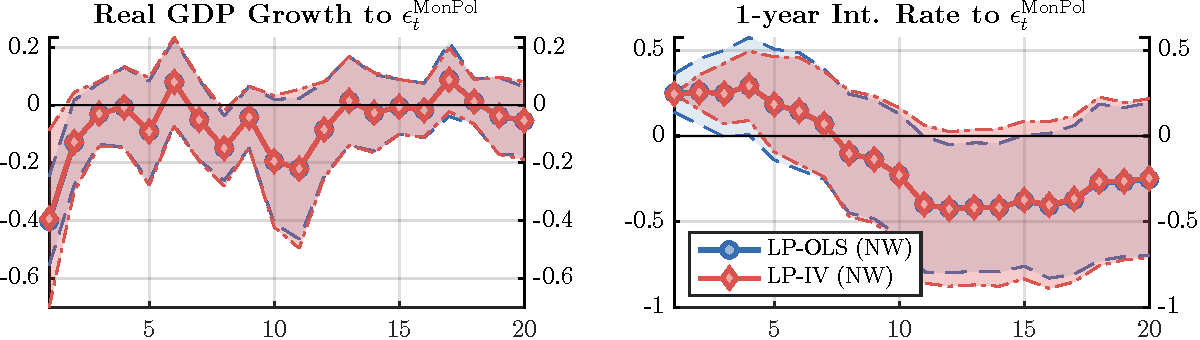
\includegraphics[width=.9\textwidth]{LP_OLS_IV}
        \end{center}
        \vspace{0.2cm}
        \caption{\scshape{Impulse Responses: LP-OLS vs.\ LP-IV}}
        \vspace{0.2cm}
        \scriptsize{{\scshape Note.} Impulse responses of GDP growth and the 1-year Treasury rate to a contractionary monetary policy shock identified with MPS, comparing LP-OLS (shock $s_t = \text{MPS}$ enters directly) and LP-IV (MPS instruments the 1-year Treasury rate $r_t$). Both sets of responses are normalized to a 25 basis point increase in the 1-year Treasury rate on impact. Shaded bands: 90\% Newey-West HAC confidence bands. Bivariate system estimated on quarterly US data, 1989:Q1--2019:Q4. Horizon: 20 quarters. Percentage points.}
        \label{fig:lp_ols_iv}
    \end{minipage}
\end{figure}

\begin{notebox}
\boxentry{Newey-West standard errors in LP}
\textbf{Newey-West standard errors in LP.} \ At horizon $h$, the LP regression error $e_{t+h}$ is the $h$-step-ahead forecast error. When the VAR lag order $p$ is correctly specified and the full $p$-lag vector $w_t$ is included as controls, the forecast error admits the moving-average representation
\begin{equation*}
    e_{t+h} = \varepsilon_{t+h} + \psi_1 \varepsilon_{t+h-1} + \cdots + \psi_{h-1}\varepsilon_{t+1},
\end{equation*}
where $\psi_k$ are the MA coefficients of the Wold representation (see Section~\ref{sec:wold}). This MA($h-1$) structure implies that $e_{t+h}$ is serially correlated with $e_{t+1}, \ldots, e_{t+h-1}$ for $h > 1$, even when the structural shocks $\varepsilon_t$ are white noise. The correct estimator is therefore a heteroskedasticity- and autocorrelation-consistent (HAC) estimator. \mci{LPmodel} uses Newey-West with bandwidth $L = h-1$, matching the exact MA order, and the reported confidence bands (\mci{INF}, \mci{SUP}) are based on \mci{bstd\_NW}.
\end{notebox}

\noindent Section~\ref{sec:lp_exog} below compares the local projection and exogenous-variable SVAR impulse responses on the same bivariate example.

\subsection{Local Projections versus VAR}\label{sec:lp_exog}

Section~\ref{sec:lp_background} established the key trade-off: LP is robust to VAR misspecification but less efficient when the VAR is correctly specified. This subsection illustrates that trade-off directly, comparing the LP-OLS impulse responses of Section~\ref{sec:lp_estimation} with those from the exogenous-variable SVAR of Section~\ref{sec:exog}. Both methods use MPS as the identification variable and produce responses to a 25 basis point increase in the 1-year Treasury rate (using the same LP-OLS normalization as in Figure~\ref{fig:lp_ols_iv}). Full details of the exogenous-variable identification scheme are in Section~\ref{sec:exog}.

The two approaches are mechanically distinct but asymptotically equivalent. In the exogenous-variable SVAR, the exogenous shock $s_t$ enters the system directly as a contemporaneous regressor in each VAR equation, and the structural impact is identified jointly with the VAR dynamics in a single estimation step. The LP estimator, by contrast, projects the $h$-step-ahead outcome directly onto $s_t$ at each horizon, without fitting a fully specified dynamic model. Under exogeneity of $s_t$ and a common lag structure, both approaches recover the same first column of $B$ at the impact horizon: at $h=0$, both reduce to the same OLS projection of each endogenous variable on $s_t$ conditional on the same lag controls, so the two estimators deliver asymptotically equivalent impact responses. Any systematic divergence between the two at horizons $h>0$ is therefore informative about potential misspecification in the VAR dynamics. \cite{PlagborgMollerWolf2021} formalize this result: LP, proxy SVAR, and exogenous-variable SVAR all identify the same population impulse responses under the same identification assumptions, provided the lag order grows with the sample size (formally, $p \to \infty$ as $T \to \infty$).

The two approaches thus present a practical trade-off. LP is agnostic about the dynamic structure at every horizon, making it robust to lag truncation and VAR misspecification. The exogenous-variable SVAR imposes cross-horizon parameter restrictions implied by the autoregressive dynamics, which delivers efficiency gains when the VAR is correctly specified but propagates any misspecification into the estimated responses at all horizons.

\vspace{0.2cm}
\begin{figure}[ht!]
	\centering%
	\begin{minipage}[b]{.9\textwidth}
		\begin{center} 
			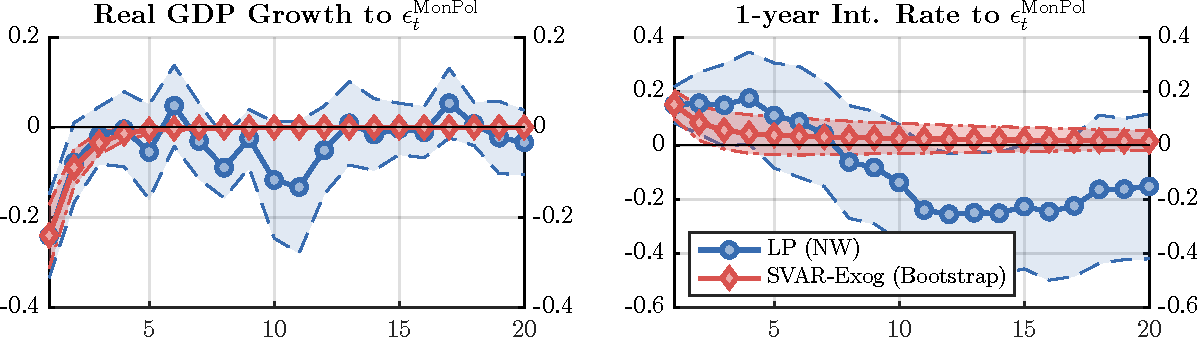
\includegraphics[width=.9\textwidth]{LP}
		\end{center}
		\vspace{0.2cm}
		\caption{\scshape{Impulse Responses: LP vs.\ Exogenous-Variable SVAR}}
		\vspace{0.2cm}
		\scriptsize{{\scshape Note.} Impulse responses of the log-difference of US real GDP and the 1-year Treasury bill yield to a contractionary monetary policy shock, comparing local projections (LP; \cite{Jorda2005}) and an exogenous-variable SVAR. Both methods use the same external instrument. LP responses are estimated horizon-by-horizon, with 90\% Newey-West HAC confidence bands (shaded area), using bandwidth $h-1$ at each horizon $h$. The exog-SVAR propagates the IV-identified impact response through the estimated VAR dynamics (solid line). Bivariate system estimated on quarterly US data, 1989:Q1--2019:Q4. Horizon: 20 quarters. Percentage points.}
		\label{fig:lp_svar}
	\end{minipage}
\end{figure}

Figure~\ref{fig:lp_svar} compares the impulse responses from the two approaches. For GDP growth, LP and the exogenous-variable SVAR track closely across horizons. For the interest rate, they diverge at longer horizons: the VAR-implied path is smoother, reflecting the cross-horizon restrictions imposed by the autoregressive dynamics, whereas the LP path is less constrained. This divergence may indicate misspecification in the VAR dynamics. LP is robust to such misspecification since it imposes no cross-horizon restrictions. When the two methods yield systematically different responses at long horizons, the divergence warrants investigation: it may signal VAR misspecification, but it may also reflect the additional estimation noise that LP incurs by fitting each horizon independently.

\section{Conclusions}

Decades after \cite{Sims1980}, VARs remain a workhorse of empirical macroeconomics. This handbook has covered the foundations of VAR analysis, from reduced-form estimation to structural identification, and from theoretical exposition to practical implementation. The guiding principle has been to explain the mechanics of VAR models by showing them at work. The exposition has walked through reduced-form and structural VARs, seven identification approaches (zero short-run restrictions, zero long-run restrictions, sign restrictions, narrative sign restrictions, external instruments, identification with exogenous variables, and combined sign-IV restrictions), and the three main tools of structural dynamic analysis (impulse responses, forecast error variance decompositions, and historical decompositions). The toolbox also provides bootstrap confidence bands for point-identified schemes and Bayesian posterior draws for sign-restricted models, allowing researchers to quantify both sampling and identification uncertainty. Local projections are covered as a specification-robust alternative to VAR-based impulse responses. Six influential applications (Appendix~\ref{sec:applications}) illustrate these methods on canonical empirical datasets.

This handbook is aimed at researchers and PhD students looking for a hands-on introduction to VAR analysis. It is not a substitute for standard time-series textbooks but a complement, intended to make those more formal treatments easier to engage with once the mechanics are concrete. The VAR literature continues to evolve rapidly, and future versions of the Toolbox will extend its coverage.

The code is public, the examples are a starting point rather than an endpoint, and users are encouraged to adapt the routines to their own research questions. Feedback and contributions via the project repository are welcome and help the Toolbox keep evolving.

A closing, more personal word. This Toolbox began as a graduate student's attempt to understand VARs by coding them line by line, and it has stayed with me through every stage of my career since. What started as a private learning device became something other people rely on---and there is real reward in seeing one's own tools put to work in someone else's hands. If this handbook helps even a few readers reach the moment when a method stops being a black box and becomes something they own, it will have done its job. 

{
\clearpage
\footnotesize
\singlespacing
\bibliographystyle{ecta}
\bibliography{BIBLIO}}

\clearpage
\appendix
\addtocontents{toc}{\protect\tocheading{Appendix}}
\numberwithin{subsection}{section}
\numberwithin{table}{section}
\numberwithin{figure}{section}
\numberwithin{equation}{section}
\setcounter{equation}{0}
\onehalfspacing



\section{Data Sources}\label{sec:data}

The spreadsheet \path{Primer_Data.xlsx}, located in \path{Primer/data/}, contains the two US time series used in the main text at quarterly frequency. The sample period is 1989:Q1 to 2019:Q4 ($T=124$ observations). All series are downloaded from FRED (Federal Reserve Bank of St. Louis).

\begin{itemize}
    \item \textbf{Real GDP} (\texttt{gdp}): Real Gross Domestic Product, seasonally adjusted annual rate (GDPC1). Source: Bureau of Economic Analysis.
    \item \textbf{1-year Treasury Bill Yield} (\texttt{i1yr}): Market Yield on US Treasury Securities at 1-Year Constant Maturity (GS1). Source: Board of Governors of the Federal Reserve System.
\end{itemize}

\noindent The baseline VAR example in the main text uses two transformed series: the log-difference of US real GDP (scaled by 100, denoted $y_t$) and the level of the 1-year Treasury Bill yield (denoted $r_t$).

\noindent The replication applications in Section~\ref{sec:applications} use separate datasets not covered here. These have been downloaded from the replication folders available online for each original paper and are stored in \path{Replic/<Author><Year>/} alongside the corresponding replication scripts. Each script (\path{GO\_<Author><Year>.m}) identifies the data source at the top of the file.

\section{Notation Summary}\label{sec:notation}

The table below lists the main mathematical symbols used in this handbook, their dimensions, the section where each is first defined, and their MATLAB counterpart where applicable. Scalars are dimensionless; all vectors are column vectors unless otherwise noted.

\begin{table}[ht!]
	\centering
	\begin{minipage}[b]{.9\textwidth}
		\begin{center}\small
		\begin{tabular}{llll}
			\toprule \addlinespace Symbol & Dimension & First defined & MATLAB \\ \midrule
			\addlinespace $k$ & scalar & \S\,\ref{sec:rfvar} & \mc{nvar} \\
			$p$ & scalar & \S\,\ref{sec:rfvar} & \mc{nlag} \\
			$T$ & scalar & \S\,\ref{sec:rfvar} & \mc{nobs} \\
			$t$ & scalar (time index) & \S\,\ref{sec:rfvar} & --- \\
			$h$ & scalar (horizon) & \S\,\ref{sec:irf} & \mc{nsteps} \\
			$x_t$ & $k\times 1$ & \S\,\ref{sec:rfvar} & \mc{ENDO(t,:)'} \\
			$c$ & $k\times 1$ (intercept) & \S\,\ref{sec:reducedform} & \mc{VAR.F(:,1)} (\mc{detc}$=1$) \\
			$\Phi_j$ & $k\times k$ (lag-$j$ coeff.) & \S\,\ref{sec:reducedform} & \mc{VAR.F(:,2:end)} \\
			$\mathcal{F}$ & $kp\times kp$ (companion) & \S\,\ref{sec:stability} & \mc{VAR.Fcomp} \\
			$u_t$ & $k\times 1$ (residuals) & \S\,\ref{sec:reducedform} & \mc{VAR.resid} \\
			$\Sigma_u$ & $k\times k$ & \S\,\ref{sec:reducedform} & \mc{VAR.sigma} \\
			$B$ & $k\times k$ (impact matrix) & \S\,\ref{sec:struct_var} & \mc{VAR.B} \\
			$\varepsilon_t$ & $k\times 1$ (struct.\ shocks) & \S\,\ref{sec:struct_var} & --- \\
			$P$ & $k\times k$ (Cholesky of $\Sigma_u$) & \S\,\ref{sec:short} & --- \\
			$P_\Omega$ & $k\times k$ (Cholesky of $\Omega$) & \S\,\ref{sec:long} & --- \\
			$Q$ & $k\times k$ (rotation) & \S\,\ref{sec:struct_var} & --- \\
			$\Omega$ & $k\times k$ (long-run cov.) & \S\,\ref{sec:long} & --- \\
			$C$ & $k\times k$ (long-run impact) & \S\,\ref{sec:long} & --- \\
			$IR_h = \Theta_h$ & $k\times k$ & \S\,\ref{sec:irf} & \mc{IR(h,:,:)} \\
			$z_t$ & scalar or $k_z\times 1$ (external instrument) & \S\,\ref{sec:iv}, \S\,\ref{sec:lp} & \mc{IV} \\
			$\delta$ & $k\times 1$ (exog.\ coeff.) & \S\,\ref{sec:exog} & --- \\
			$s_t$ & scalar (shock, enters directly) & \S\,\ref{sec:exog}, \S\,\ref{sec:lp} & \mc{exoshock}, \mc{TREAT} \\
			$d_t$ & scalar (endog.\ treatment, LP-IV) & \S\,\ref{sec:lp} & \mc{TREAT} \\
			$H$ & scalar (max LP horizon) & \S\,\ref{sec:lp} & \mc{nsteps} \\
			$\beta_h$ & scalar (LP coefficient at horizon $h$) & \S\,\ref{sec:lp} & \mc{IR(h)} \\
			$x_{i,t+h}$ & scalar ($i$-th LP outcome at horizon $h$) & \S\,\ref{sec:lp} & \mc{ENDO} \\
			$w_t$ & $n_w\times 1$ (LP control vector) & \S\,\ref{sec:lp} & \mc{CTRL} \\
			$e_{t+h}$ & scalar (LP regression error) & \S\,\ref{sec:lp} & --- \\ \bottomrule
		\end{tabular}%
		\end{center} 
		\vspace{0.4cm}
		\caption{\scshape{Notation Summary}}
		\vspace{0.2cm}
		\scriptsize{{\scshape Note.} The companion matrix $\mathcal{F}$ is $kp\times kp$: the upper $k$ rows collect $[\Phi_1,\ldots,\Phi_p]$ and the lower $k(p-1)$ rows form the identity-shift block $[I_{k(p-1)},\,0]$ (see Box~\ref{box:companion}). The impulse response matrix $IR_h = \Theta_h = \Phi^h B$ for a VAR(1); for a general VAR($p$), replace $\Phi^h B$ with $\mathcal{F}^h \mathcal{B}$ where $\mathcal{F}$ is the companion matrix and $\mathcal{B}$ is the impact matrix $B$ padded with zeros to dimension $kp\times k$ (see Box~\ref{box:companion}).}
		\label{tab:notation}
	\end{minipage}
\end{table}


\section{Applications and Replications}\label{sec:applications}

The applications and replications in this section complement the theoretical exposition in the main text by showing the identification methods at work on canonical empirical datasets. The simple bivariate VAR used throughout the handbook serves a purely pedagogical purpose: with only two variables and one lag, the algebra remains transparent and the mechanics of the toolbox are not obscured by complexity. These six applications take a step closer to genuine empirical practice. 

Each replication selects a canonical study from the VAR literature, reproduces its key findings using the VAR Toolbox, and connects the implementation to the identification methods developed in the main text. The first five replications span the main SVAR identification strategies: recursive identification \citep{StockWatson2001}, long-run restrictions \citep{BlanchardQuah1989}, sign restrictions \citep{Uhlig2005}, narrative sign restrictions \citep{AntolinDiazRubioRamirez2018}, and external instruments \citep{GertlerKaradi2015}. The sixth replication illustrates local projection methods (both LP-OLS and LP-IV) following the treatment in \cite{JordaTaylor2025}. 

Replication scripts are stored in \path{Replic/} and named \path{GO\_<Author><Year>.m}. The MATLAB boxes below show concise snippets that highlight the key steps of each application. The complete executable code, including data loading, transformations, and figure options, is in \path{Primer/VARToolbox\_Primer.m}.\footnote{Sections~11--15 of \path{VARToolbox\_Primer.m} replicate Stock and Watson (2001), Blanchard and Quah (1989), Uhlig (2005), Antol\'{i}n-D\'{i}az and Rubio-Ram\'{i}rez (2018), and Gertler and Karadi (2015), respectively. The sixth replication (Jord\`{a} and Taylor, 2025) is in the dedicated script \path{Replic/GO\_JT2025.m} and is not covered in the Primer.}

%------------------------------------------
\subsection{Stock and Watson (2001): Zero Short-Run Restrictions}\label{sec:app_sw}

What are the effects of monetary policy shocks on inflation and unemployment? \cite{StockWatson2001} address this question using a trivariate VAR estimated on quarterly US data from 1960:Q1 to 2000:Q4. The three endogenous variables are inflation ($\pi_t = 400(\log P_t - \log P_{t-1})$, annualized quarterly log change in the chain-weighted GDP price index), the unemployment rate ($u_t$, percent), and the federal funds rate ($r_t$, percent at annual rate). The specification is a VAR(4) with a constant.

The identification strategy rests on two timing assumptions. First, the policy rate can respond contemporaneously to inflation and unemployment, reflecting the Federal Reserve's ability to observe current-quarter macroeconomic conditions, so the federal funds rate is ordered last. Second, monetary policy shocks have no contemporaneous effect on inflation or unemployment, reflecting the well-known long and variable lags of monetary transmission. Together, these assumptions imply a lower-triangular impact matrix $B$:
\begin{equation}
\begin{bmatrix}
\pi_t \\
u_t \\
r_t
\end{bmatrix}
= \sum_{p=1}^{4} \Phi_p x_{t-p} +
\begin{bmatrix}
b_{11} & 0 & 0 \\
b_{21} & b_{22} & 0 \\
b_{31} & b_{32} & b_{33}
\end{bmatrix}
\begin{bmatrix}
\varepsilon_t^{1} \\
\varepsilon_t^{2} \\
\varepsilon_t^{MonPol}
\end{bmatrix}
\end{equation}
The lower-triangular structure is implemented by a Cholesky decomposition of the reduced-form covariance matrix $\Sigma_u = BB'$; see Section~\ref{sec:short} for the algebraic derivation. Inflation is ordered first, unemployment second, and the policy rate third, reflecting the assumption that the inflation and unemployment shocks are unaffected by the monetary policy shock on impact, while the federal funds rate can respond to their contemporaneous values.

Assuming the data have been loaded into the \mc{DATA} struct, the key implementation steps are:

\begin{matlabcode}
% Data and lag order
X = [DATA.infl, DATA.unemp, DATA.ff]; 
nlags = 4;  detc = 1;
% Identification setup and impulse responses with bootstrap bands
VARopt = VARoption;
VARopt.vnames    = {'Inflation','Unemployment','Fed Funds'};
VARopt.nsteps    = 24;
VARopt.snames    = {bfeps('1'), bfeps('2'), bfeps('MonPol')};
VARopt.ident     = 'short';
VARopt.inference = 1;
\end{matlabcode}

\noindent Identification and the computation and plotting of the impulse responses then follow from the usual lines of code:

\begin{matlabcode}
VAR = VARmodel(X, nlags, detc, VARopt);
VARirplot(VAR.IRbar, VARopt, VAR.IRinf, VAR.IRsup);
\end{matlabcode}

Figure~\ref{fig:SW_IR_3} reports the impulse responses to the three identified shocks. The identified monetary policy shock delivers the expected pattern: a contractionary shock raises the federal funds rate and, after a lag, increases unemployment and lowers inflation. 

\vspace{0.2cm}
\begin{figure}[ht!]
	\centering%
	\begin{minipage}[b]{.9\textwidth}
		\begin{center}
			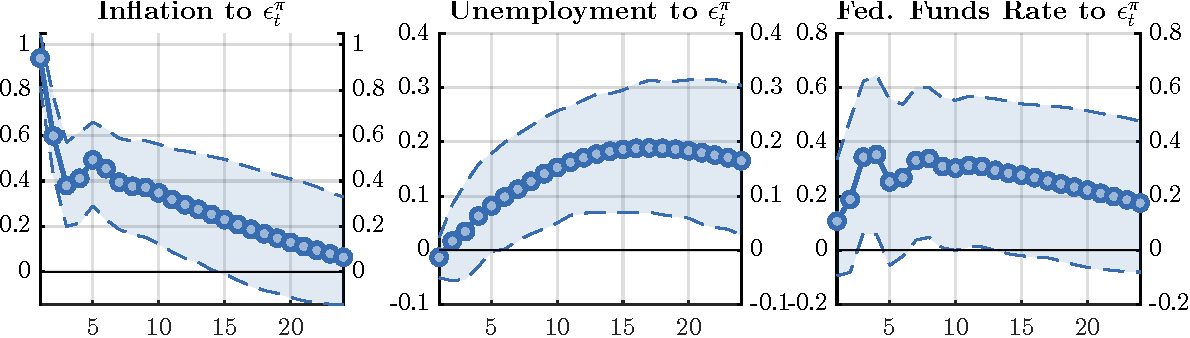
\includegraphics[width=.9\textwidth]{SW_Fig1_1}
			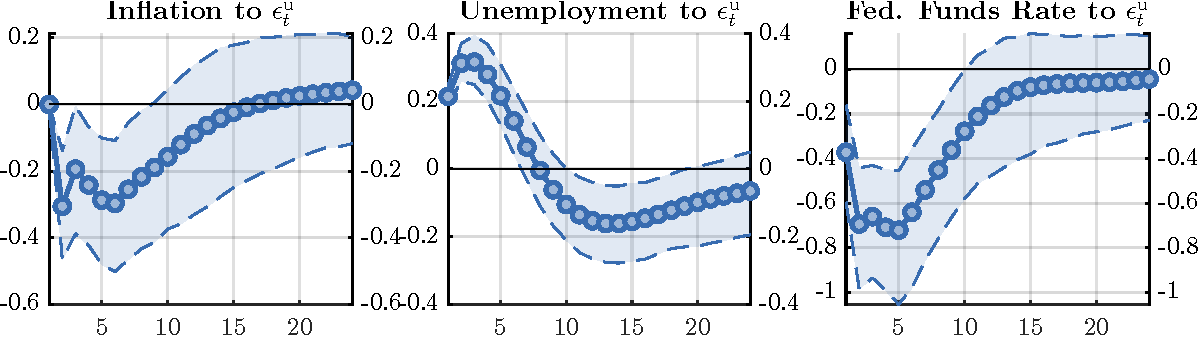
\includegraphics[width=.9\textwidth]{SW_Fig1_2}
			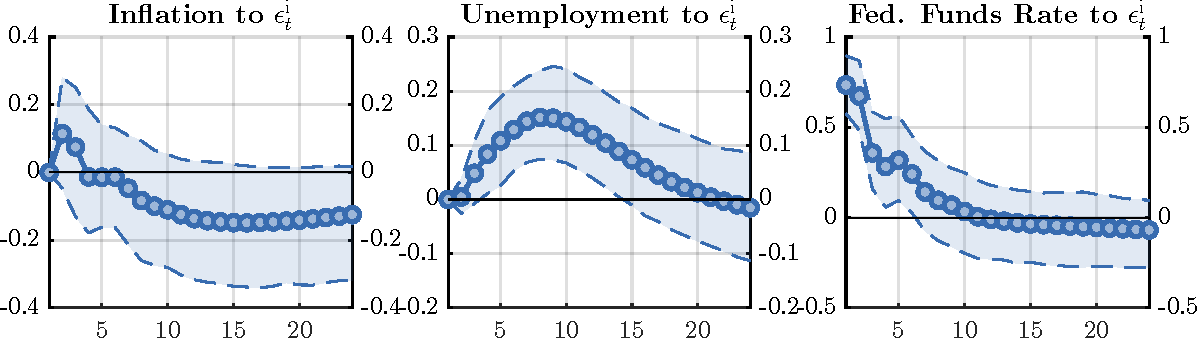
\includegraphics[width=.9\textwidth]{SW_Fig1_3}
		\end{center}%
		\vspace{0.2cm}
		\caption{\scshape{Stock and Watson (2001): Figure~3}}
		\vspace{0.2cm}
		\scriptsize{{\scshape Note.} Impulse responses of inflation, unemployment, and the federal funds rate to three shocks identified by zero contemporaneous restrictions (Cholesky). Trivariate VAR(4) with constant, estimated on quarterly US data, 1960:Q1--2000:Q4. Horizon: 24 quarters. Solid line: bootstrap mean. Shaded bands: 95\% bootstrap confidence intervals.}
		\label{fig:SW_IR_3}
	\end{minipage}
\end{figure}

\noindent The other two shocks carry no a priori economic label: they are simply the remaining orthogonal components defined by the Cholesky ordering. Their impulse responses suggest supply- and demand-like patterns, but these labels are \textit{ex post} interpretations rather than identifying restrictions. This is a general limitation of recursive identification: the chosen variable order embeds strong timing assumptions that determine which shocks are identified and how, and the economic content of each shock depends on that choice.



%------------------------------------------
\subsection{Blanchard and Quah (1989): Zero Long-Run Restrictions}\label{sec:app_bq}

How do aggregate supply and demand shocks differ in their effects on output and unemployment? \cite{BlanchardQuah1989} exploit the long-run neutrality of demand shocks implied by classical macroeconomic theory to answer this question. Using quarterly US data from 1948:Q1 to 1987:Q4, they estimate a VAR(8) with a constant that includes two variables: real GNP growth ($\Delta y_t$, percent at quarterly rate) and the unemployment rate ($u_t$, percent). The VAR is specified in growth rates for output, not levels, which matters for how the long-run restriction is expressed.

The key identifying assumption is that demand shocks have no long-run effect on the level of output, while supply shocks do. The restriction imposes long-run neutrality of demand shocks: their cumulative effect on the level of output is zero. The classical interpretation is that in the long run, output is governed by supply-side factors such as technology and capital accumulation, while demand shocks produce only transitory fluctuations. Since the VAR is in growth rates, the restriction on output levels translates into a zero cumulative impulse response of output growth to the demand shock. In matrix notation, the long-run impact matrix must be lower triangular:
\begin{equation}
\begin{bmatrix}
\Delta y_{t,t+\infty} \\
u_{t,t+\infty}
\end{bmatrix}
=
\begin{bmatrix}
c_{11} & 0 \\
c_{21} & c_{22}
\end{bmatrix}
\begin{bmatrix}
\varepsilon_t^{Supply} \\
\varepsilon_t^{Demand}
\end{bmatrix}
\end{equation}
where $C \equiv (I-\Phi)^{-1}B$ is the long-run impact matrix defined in equation~\eqref{eq:long4} of Section~\ref{sec:long}. The zero upper-right element $c_{12} = 0$ imposes long-run neutrality of demand shocks on output, which is why output growth is ordered first; no restriction is placed on the long-run response of unemployment to either shock. See Section~\ref{sec:long} for the algebraic derivation.

Assuming the data have been loaded into the \mc{DATA} struct, the key implementation steps are:

\begin{matlabcode}
% Data and lag order
X = [DATA.y, DATA.u]; % GDP growth, unemployment
nlags = 8;  detc = 1;
% Identification setup and impulse responses with bootstrap bands
VARopt = VARoption;
VARopt.vnames    = {'GDP growth','Unemployment'};
VARopt.nsteps    = 40;
VARopt.frequency = 'q';
VARopt.snames    = {bfeps('Supply'), bfeps('Demand')};
VARopt.ident     = 'long';
VARopt.inference = 1;
\end{matlabcode}

\noindent Identification and the computation and plotting of the impulse responses then follow from the usual lines of code:

\begin{matlabcode}
VAR = VARmodel(X, nlags, detc, VARopt);
VARirplot(VAR.IRbar, VARopt, VAR.IRinf, VAR.IRsup);
\end{matlabcode}

\noindent Figure~\ref{fig:BQ_IR} reports the impulse responses to the two identified shocks: the supply shock (panel A) and the demand shock (panel B). Each panel plots the responses of output growth and the unemployment rate, with the solid line denoting the bootstrap mean and the shaded bands the 95\% bootstrap confidence intervals.

\vspace{0.2cm}
\begin{figure}[ht!]
    \centering%
    \begin{minipage}[b]{.9\textwidth}
        \begin{center}
			\small \scshape(A) Supply shock \\
			\vspace{0.2cm}
            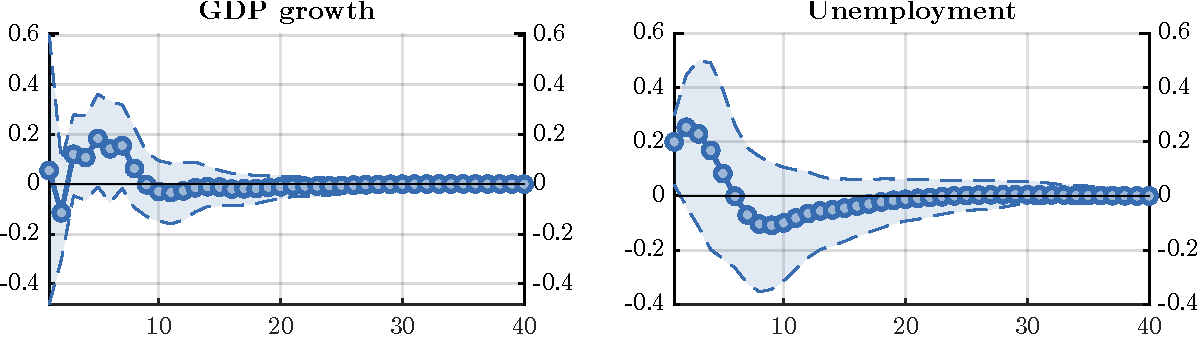
\includegraphics[width=.9\textwidth]{BQ_1}
            \\\vspace{0.4cm}
			(B) Demand shock \\
			\vspace{0.2cm}
            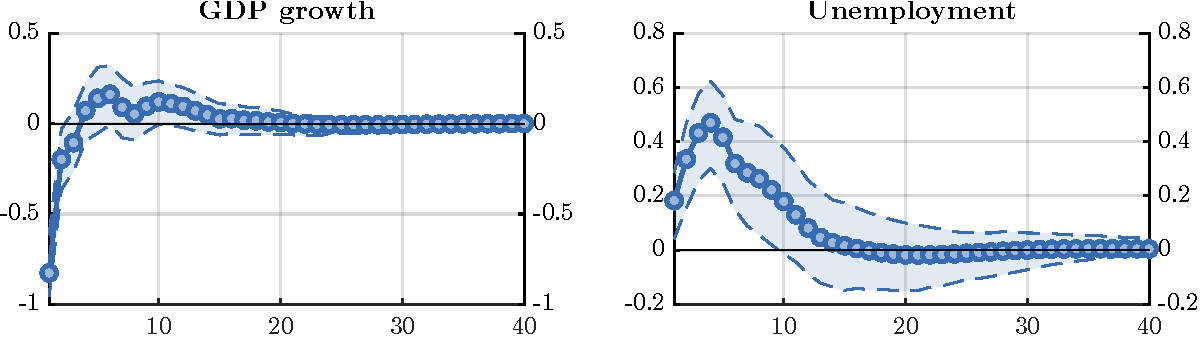
\includegraphics[width=.9\textwidth]{BQ_2}
        \end{center}
        \vspace{0.2cm}
        \caption{\scshape{Impulse Responses to a Supply and a Demand Shock}}
        \vspace{0.2cm}
        \scriptsize{{\scshape Note.} Impulse responses of US real GNP growth and the unemployment rate to a supply shock (panel A) and a demand shock (panel B), identified by zero long-run restrictions. Bivariate VAR(8) with constant, estimated on quarterly US data, 1948:Q1--1987:Q4. Horizon: 40 quarters. Solid line: bootstrap mean. Shaded area: 95\% bootstrap confidence intervals.}
        \label{fig:BQ_IR}
    \end{minipage}
\end{figure}

Figure~\ref{fig:BQ_Replication} reports the \textit{cumulative} impulse responses, obtained by cumulating the responses of output growth into the implied response of the output level. Plotting the responses in cumulative form makes the identifying restriction directly visible: the cumulative response of output to the demand shock converges to zero at long horizons, exactly as imposed by long-run neutrality, while the response to the supply shock settles at a non-zero level. The identified supply shock thus produces a permanent increase in output --- the cumulative impulse response of GDP growth converges to a positive value, reflecting a lasting shift in productive capacity.

\vspace{0.2cm}
\begin{figure}[ht!]
	\centering%
	\begin{minipage}[b]{.9\textwidth}
		\begin{center}
			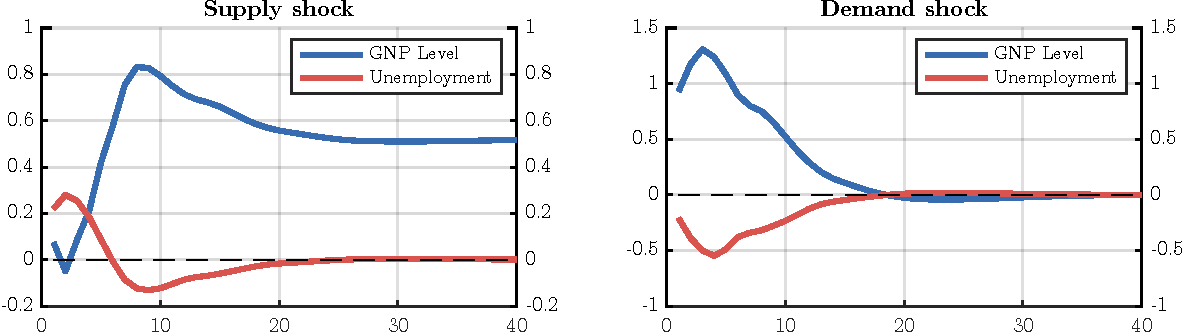
\includegraphics[width=.9\textwidth]{BQ_Fig1Fig2}
		\end{center}%
		\vspace{0.2cm}
		\caption{\scshape{Blanchard and Quah (1989): Figures~1 and~2}}
		\vspace{0.2cm}
		\scriptsize{{\scshape Note.} Impulse responses of the GNP level (cumulative sum of GNP growth responses) and the unemployment rate to supply and demand shocks identified by long-run restrictions. Bivariate VAR(8) with constant, estimated on quarterly US data, 1948:Q1--1987:Q4. Horizon: 40 quarters. Solid line: bootstrap mean. The cumulative response of GNP growth to the demand shock converges to zero by construction.}
		\label{fig:BQ_Replication}
	\end{minipage}
\end{figure}

\noindent The demand shock has no long-run effect on output by construction, but lowers unemployment on impact and drives it back toward baseline over subsequent quarters --- a pattern consistent with transitory demand fluctuations. These patterns align with the classical supply--demand dichotomy: supply shocks permanently shift the productive frontier, while demand shocks trace out cyclical fluctuations around it. What makes the exercise instructive is that a single long-run exclusion restriction --- demand shocks are neutral for the level of output --- suffices to separate permanent from transitory sources of fluctuations, with no restriction imposed on the short-run dynamics.



%------------------------------------------
\subsection{Uhlig (2005): Sign Restrictions}\label{sec:app_uhlig}

What are the effects of monetary policy on output? \cite{Uhlig2005} revisits this classic question with a deliberately agnostic approach. Rather than relying on timing assumptions or long-run restrictions, Uhlig imposes only sign restrictions that capture conventional wisdom about monetary transmission, allowing the data to speak more freely about the output effects of monetary policy (see Section~\ref{sec:sr}).

Using monthly US data from 1965:M1 to 2003:M12, Uhlig estimates a VAR(12) with a constant that includes six variables: real GDP ($rgdp_t$, log, interpolated at monthly frequency), the GDP deflator ($p_t$, log), a commodity price index ($p_t^{com}$, log), total reserves ($tr_t$, log), non-borrowed reserves ($nbr_t$, log), and the federal funds rate ($ff_t$, percent). Log-level variables are scaled by 100. The sign restrictions on impulse responses, imposed for $h = 0, 1, \ldots, 5$ (six months), are shown in equation~\eqref{eq:Uhlig_SR}: $+$ and $-$ denote required signs; $?$ denotes no restriction. Any rotation matrix $Q_j$ producing responses that violate these restrictions at any of the first six horizons is discarded; see Section~\ref{sec:sr} for the algorithm. No restriction is imposed on industrial production --- the variable of interest --- allowing the data to determine its response freely. In practice, the restrictions look like as follows:
\begin{equation}
\label{eq:Uhlig_SR}
\begin{bmatrix}
rgdp_t \\ p_t \\ p_t^{com} \\ tr_t \\ nbr_t \\ ff_t
\end{bmatrix}
= \sum_{p=1}^{12} \Phi_p x_{t-p} +
\begin{bmatrix}
{?} & {?} & {?} & {?} & {?} & {?} \\
{-} & {?} & {?} & {?} & {?} & {?} \\
{-} & {?} & {?} & {?} & {?} & {?} \\
{?} & {?} & {?} & {?} & {?} & {?} \\
{-} & {?} & {?} & {?} & {?} & {?} \\
{+} & {?} & {?} & {?} & {?} & {?}
\end{bmatrix}
\begin{bmatrix}
\varepsilon_t^{MonPol} \\ \varepsilon_t^{2} \\ \varepsilon_t^{3} \\ \varepsilon_t^{4} \\ \varepsilon_t^{5} \\ \varepsilon_t^{6}
\end{bmatrix}
\end{equation}

\noindent In the VAR Toolbox, sign restrictions are encoded in a matrix \mc{R} with rows for variables and columns for shocks. Only the first column (the monetary policy shock) carries non-zero entries; the remaining columns are zero, leaving the other five shocks unrestricted. The option \mc{VARopt.sr\_hor = 6} enforces the restrictions for the first 6 months. Assuming the data have been loaded into the \mc{DATA} struct, the key implementation steps are:

\begin{matlabcode}
% Data and lag order
X = [DATA.y, DATA.pi, DATA.comm, DATA.res, DATA.nbres, DATA.ff];
nlags = 12;  detc = 1;
% Identification setup and impulse responses
VARopt = VARoption;
VARopt.ndraws    = 500;
VARopt.sr_hor    = 6;
VARopt.inference = 1;  
VARopt.nsteps    = 60;
VARopt.frequency = 'm';
VARopt.pctg      = 68;
VARopt.snames    = {bfeps('MonPol')};
% R: 1 = positive, -1 = negative, 0 = unrestricted
R = [ 0, 0, 0, 0, 0, 0;   % Industrial production (unrestricted)
     -1, 0, 0, 0, 0, 0;   % GDP Deflator (negative)
     -1, 0, 0, 0, 0, 0;   % Commodity Prices (negative)
      0, 0, 0, 0, 0, 0;   % Total Reserves (unrestricted)
     -1, 0, 0, 0, 0, 0;   % NonBorr. Reserves (negative)
      1, 0, 0, 0, 0, 0];  % Fed Funds (positive)
% Identify with sign restrictions
VARopt.ident = 'sign';
VARopt.R = R;
\end{matlabcode}

\noindent Identification and the computation and plotting of the impulse responses then follow from the usual lines of code:

\begin{matlabcode}
VAR_sr = VARmodel(X, nlags, detc, VARopt);
VARirplot(VAR_sr.IRmed, VARopt, VAR_sr.IRinf, VAR_sr.IRsup);
\end{matlabcode}

\vspace{0.2cm}
\begin{figure}[ht!] 
	\centering%
	\begin{minipage}[b]{.9\textwidth}
		\begin{center}
			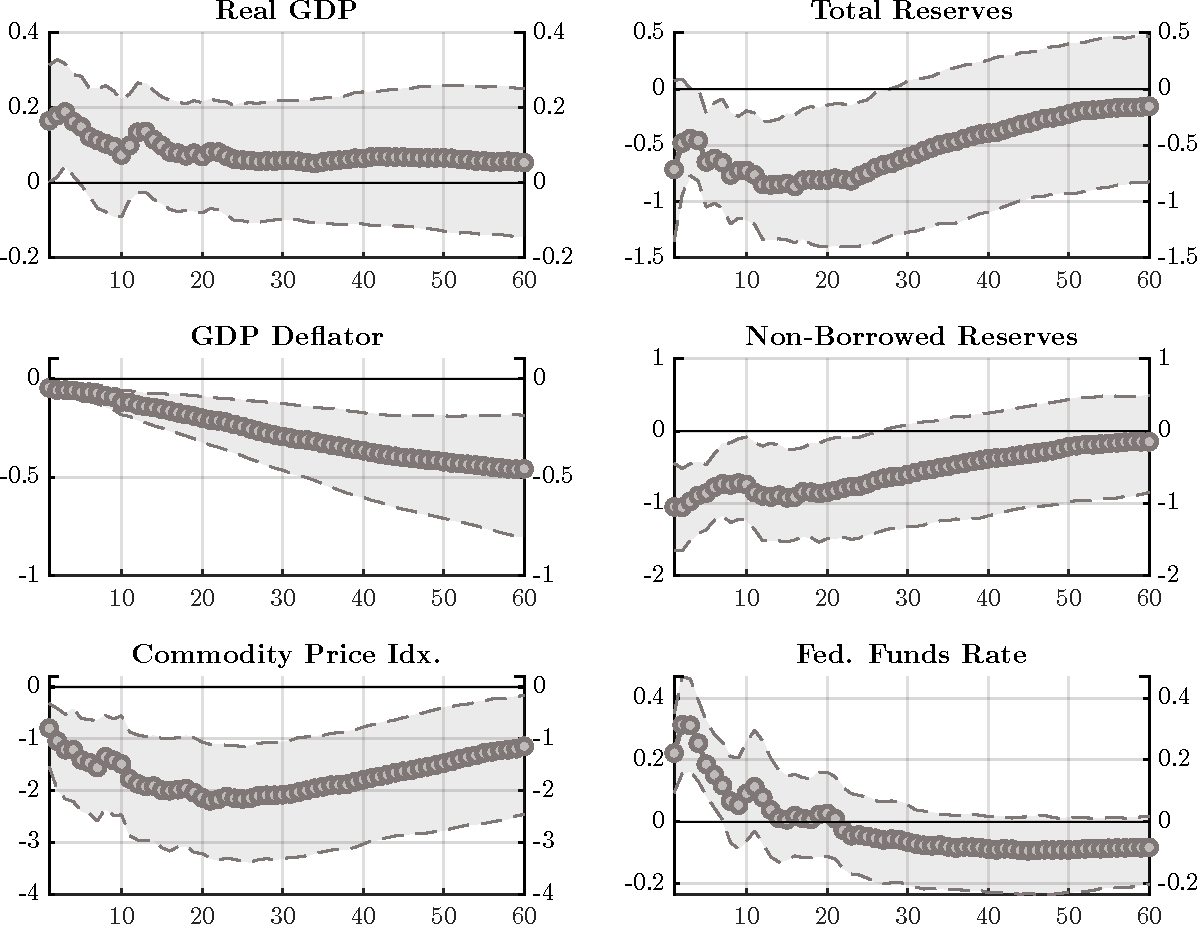
\includegraphics[width=.9\textwidth]{Uhlig_Fig6}
		\end{center}%
		\vspace{0.2cm}
		\caption{\scshape{Uhlig (2005): Figure~6}}
		\vspace{0.2cm}
		\scriptsize{{\scshape Note.} Impulse responses of industrial production, the GDP deflator, a commodity price index, total reserves, non-borrowed reserves, and the federal funds rate to a contractionary monetary policy shock identified by sign restrictions. Six-variable VAR(12) with constant, estimated on monthly US data, 1965:M1--2003:M12. Horizon: 60 months. Solid line: element-wise median (\mci{VAR\_sr.IRmed}); shaded bands: 68\% credible intervals (16th--84th percentiles). No restriction is imposed on industrial production.} 
		\label{fig:Uhlig_Replication}
	\end{minipage}
\end{figure}

Figure~\ref{fig:Uhlig_Replication} reports the impulse responses to the contractionary monetary policy shock. The key finding is that the output response is ambiguous: while the restricted variables respond as assumed --- the federal funds rate rises, the price level and non-borrowed reserves fall --- the impulse response of industrial production (top-left panel) is highly uncertain, with the 68\% credible interval spanning both positive and negative values. Uhlig interprets this as evidence that the data, under minimal identifying restrictions, do not deliver a clear verdict on the output effects of monetary policy.

Two features of the figure are worth emphasizing for interpretation. First, the model is set-identified: each accepted rotation $Q_j$ generates one admissible impulse response, and the shaded bands trace the 16th--84th percentiles of the responses across all accepted draws (\mc{VAR\_sr.IRinf} and \mc{VAR\_sr.IRsup}), with the solid line the element-wise median (\mc{VAR\_sr.IRmed}). The bands thus summarize identification (rotation) uncertainty and, when \mc{VARopt.inference = 1}, sampling uncertainty as well; they are not the confidence intervals of a single point estimate. Second, the restricted responses carry the imposed sign over the constrained horizons $h = 0, \ldots, 5$ by construction, whereas their behavior at longer horizons --- and the entire path of real GDP --- is governed by the estimated reduced-form dynamics. The contrast between the tightly signed responses of the restricted variables and the diffuse response of industrial production is precisely what the agnostic identification is designed to surface.

%------------------------------------------
\subsection{Antol\'{i}n-D\'{i}az and Rubio-Ram\'{i}rez (2018):\\ Narrative Sign Restrictions}\label{sec:app_nsr}

Can narrative evidence about specific historical episodes sharpen inference from sign restrictions? \cite{AntolinDiazRubioRamirez2018} propose to augment the standard sign restrictions approach with \textit{narrative restrictions} --- additional constraints tied to well-documented historical events. They apply this idea to the Uhlig (2005) six-variable monetary VAR, retaining the same sign restrictions but extending the sample to 1965:M1--2007:M11 and estimating without a constant (following footnote~8 of \citealt{AntolinDiazRubioRamirez2018}, p.~27, who demean the data prior to estimation). The additional identifying information comes from October 1979, the month of the Volcker disinflation announcement.

Historical records leave little doubt about two facts regarding that episode. First, the monetary policy shock was strongly positive: the Fed tightened aggressively and unexpectedly. Second, monetary policy was the dominant driver of the unexpected movement in the federal funds rate that month, with no comparably large competing shocks. These two observations motivate two narrative restrictions targeted at 1979:M10:
\begin{itemize}
\item \text{Type~1 (sign):}\quad  $\varepsilon_{1979:M10}^{MonPol} > 0$ \bigskip
\item \text{Type~2 (dominance):}\quad  $\bigl|b_{6m}\,\varepsilon_{1979:M10}^{MonPol}\bigr| > \textstyle\sum_{k\neq m}\bigl|b_{6k}\,\varepsilon_{k,1979:M10}\bigr|$
\end{itemize}
where $b_{6m}$ is the element of $B$ in row~6 (federal funds rate) and column~$m$ (monetary policy shock), so each product $b_{6k}\,\varepsilon_{k,1979:M10}$ measures the contribution of structural shock $k$ to the federal funds rate residual in that month. The Type~2 inequality therefore requires the monetary policy shock to account for more of the unexpected movement in the federal funds rate than all other shocks combined. Any candidate rotation matrix $Q_j$ that satisfies the sign restrictions but violates any narrative constraint is discarded. See Section~\ref{sec:narr} for the algebraic formulation and acceptance-rejection algorithm.

In the VAR Toolbox, narrative restrictions are passed to \mc{VARmodel} via \mc{VARopt.R}, a struct \mc{R} combining the sign restriction matrix with the narrative fields \mc{R.narr\_sign} and \mc{R.narr\_dom}. Assuming the data have been loaded into the \mc{DATA} struct, the key implementation steps are:

\begin{matlabcode}
% Data and lag order
X = [DATA.y, DATA.pi, DATA.comm, DATA.res, DATA.nbres, DATA.ff];
nlags = 12;  detc = 0;
% Identification setup and impulse responses
VARopt = VARoption;
VARopt.nsteps = 60;
VARopt.sr_hor = 6;
VARopt.snames = {bfeps('MonPol')};
VARopt.dates  = dates;
% Sign restrictions matrix (column 1: MP shock)
R.sign = [ 0, 0, 0, 0, 0, 0;
          -1, 0, 0, 0, 0, 0;
          -1, 0, 0, 0, 0, 0;
           0, 0, 0, 0, 0, 0;
          -1, 0, 0, 0, 0, 0;
           1, 0, 0, 0, 0, 0];
% Type 1: MP shock positive at October 1979
R.narr_sign.shock  = 1;
R.narr_sign.period = '1979m10';
R.narr_sign.sign   = 1;
% Type 2: MP shock dominant for ff at October 1979
R.narr_dom.shock  = 1;
R.narr_dom.period = '1979m10';
R.narr_dom.var    = 6;
% Identify with sign + narrative restrictions
VARopt.ident = 'sign';
VARopt.R = R;
\end{matlabcode}

\noindent Identification and the computation and plotting of the impulse responses then follow from the usual lines of code:

\begin{matlabcode}
VAR_nsr = VARmodel(X, nlags, detc, VARopt);
VARirplot(VAR_nsr.IRmed, VARopt, VAR_nsr.IRinf, VAR_nsr.IRsup);
\end{matlabcode}

Figure~\ref{fig:ADRR_Replication} reports the impulse responses to the contractionary monetary policy shock under sign restrictions alone (blue) and under sign plus narrative restrictions (red). Adding the October 1979 narrative restrictions substantially narrows the identified set relative to sign restrictions alone: the red credible bands are noticeably tighter than the blue ones, and the central estimates shift. Both effects reflect the same mechanism: candidates that satisfy the sign restrictions but are inconsistent with the Volcker episode are discarded, leaving a smaller and differently located set of admissible impulse responses. 

In particular, monetary policy now has a clear effect on output: the sign-only response (blue, top-left panel) is positive or indeterminate, whereas the narrative restrictions push the median output response (red) below zero at medium and longer horizons, so that a contractionary monetary policy shock now lowers output --- resolving the ambiguity left by the agnostic identification of \cite{Uhlig2005}. The result is sharper inference about the effects of monetary policy, achieved by conditioning on one well-documented historical episode.

\vspace{0.2cm}
\begin{figure}[ht!]
	\centering%
	\begin{minipage}[b]{.9\textwidth}
		\begin{center}
			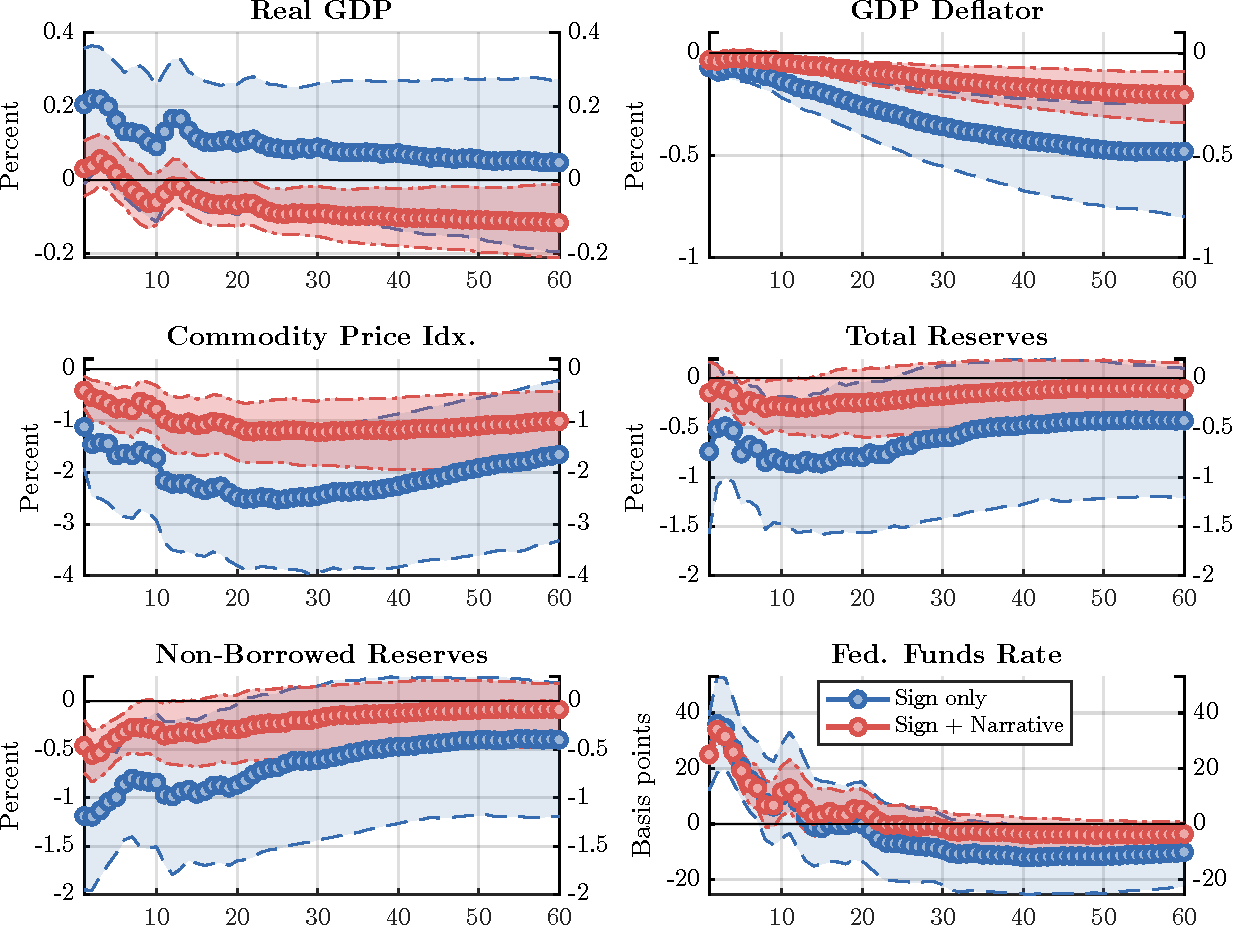
\includegraphics[width=.9\textwidth]{ADRR_Fig6}
		\end{center}%
		\vspace{0.2cm}
		\caption{\scshape{Antol\'{i}n-D\'{i}az and Rubio-Ram\'{i}rez (2018): Figure~8}}
		\vspace{0.2cm}
		\scriptsize{{\scshape Note.} Impulse responses to a contractionary monetary policy shock: sign restrictions alone (blue) versus sign restrictions augmented with narrative restrictions (red). Six-variable VAR(12) without constant, estimated on monthly US data, 1965:M1--2007:M11. Horizon: 60 months. Shaded bands: 68\% credible intervals. Narrative restrictions target October 1979 (Volcker reform): Type~1 requires a positive monetary policy shock; Type~2 requires that shock to be the dominant driver of the federal funds rate that month.}
		\label{fig:ADRR_Replication}
	\end{minipage}
\end{figure}


The mechanism is seen most directly in the distribution of the identified monetary policy shock at the targeted date. Figure~\ref{fig:ADRR_ShockDist} plots, across accepted draws, the structural monetary policy shock in October 1979 under sign restrictions alone (blue) and under sign plus narrative restrictions (red). Under sign restrictions alone the shock is roughly symmetric about zero, so the data are consistent with either an expansionary or a contractionary impulse in that month. The narrative restrictions truncate and reshape this distribution: Type~1 discards every draw with a non-positive shock, removing all mass to the left of zero, while Type~2 retains only draws in which the monetary policy shock dominates the federal funds rate movement, concentrating the surviving mass on large positive values. The tighter impulse response bands in Figure~\ref{fig:ADRR_Replication} are the downstream consequence of this reweighting of the admissible draws.

\vspace{0.2cm}
\begin{figure}[ht!]
	\centering%
	\begin{minipage}[b]{.9\textwidth}
		\begin{center}
			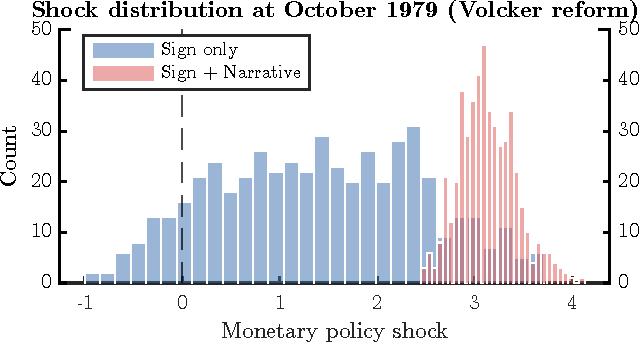
\includegraphics[width=.6\textwidth]{ADRR_Fig5}
		\end{center}%
		\vspace{0.2cm}
		\caption{\scshape{Antol\'{i}n-D\'{i}az and Rubio-Ram\'{i}rez (2018): Distribution of the monetary policy shock at October 1979}}
		\vspace{0.2cm}
		\scriptsize{{\scshape Note.} Distribution of the structural monetary policy shock in October 1979 (the Volcker reform) across accepted draws. Blue: sign restrictions only. Red: sign restrictions augmented with narrative restrictions. The shock is recovered as $\varepsilon = B^{-1}u$ from the reduced-form residuals $u$ and each accepted impact matrix $B$, in structural shock units (not normalized to the 25~basis-point federal funds impact used for the impulse responses). The dashed vertical line at zero marks the boundary imposed by the Type~1 narrative restriction ($\varepsilon^{MonPol}_{1979:M10} > 0$).}
		\label{fig:ADRR_ShockDist}
	\end{minipage}
\end{figure}

%------------------------------------------
\subsection{Gertler and Karadi (2015): External Instruments}\label{sec:app_gk}

How does monetary policy affect credit markets? \cite{GertlerKaradi2015} focus on the credit channel of monetary transmission, exploiting high-frequency movements in asset prices around FOMC announcements to identify monetary policy shocks cleanly.

Using monthly US data from 1979:M7 to 2012:M6, they estimate a VAR(12) with a constant that includes four variables: the 1-year Treasury bill rate (percent), the consumer price index (log), industrial production (log), and the excess bond premium (percent). The excess bond premium (EBP), constructed by \cite{GilchristZakrajsek2012}, measures the component of corporate credit spreads orthogonal to expected default risk; it captures financial market frictions and tightening credit conditions. The policy rate is placed first in the variable ordering; this is required by the VAR Toolbox implementation, which instruments the residual of the first variable, and does not reflect a theoretical restriction of the external-instrument approach.

The instrument is constructed from changes in federal funds futures prices in a narrow window around FOMC announcements:
\begin{equation*}
z_t = -(P_{t,\tau+20} - P_{t,\tau-10})
\end{equation*}
where $P_{t,\tau}$ is the futures price at time $\tau$ (measured in minutes relative to the announcement) on day $t$. The subscripts $\tau-10$ and $\tau+20$ define a 30-minute window; the negative sign converts a futures price increase into a positive rate reading, since futures prices move inversely to interest rates, so $z_t > 0$ corresponds to an unexpected policy tightening. The instrument must satisfy relevance ($\mathbb{E}[\varepsilon_t^{MonPol} z_t'] \neq 0$) and exogeneity ($\mathbb{E}[\varepsilon_t^i z_t'] = 0$ for $i \neq \text{MonPol}$). See Section~\ref{sec:iv} for the identification argument. Assuming the data have been loaded into the \mc{DATA} struct, the key implementation steps are:

\begin{matlabcode}
% Data, instrument, and lag order
X  = [DATA.gs1, DATA.logcpi, DATA.logip, DATA.ebp];
IV = DATA.ff4_tc;  % FF4 futures surprise
nlags = 12;  detc = 1;
% Options
VARopt = VARoption;
VARopt.nsteps    = 48;
VARopt.frequency = 'm';
VARopt.method    = 'wild';
VARopt.ndraws    = 500;
VARopt.inference = 1;
VARopt.pick      = 1;
% (1) Recursive (Cholesky) identification: policy rate ordered first
VARopt.ident     = 'short';
VAR_chol = VARmodel(X, nlags, detc, VARopt);
% (2) External-instrument identification (proxy SVAR)
VARopt.ident     = 'iv';
VARopt.IV        = IV;
VAR_iv   = VARmodel(X, nlags, detc, VARopt);
\end{matlabcode}

Figure~\ref{fig:GK_IR_1} reproduces the central comparison of \cite{GertlerKaradi2015}: the same four-variable VAR(12) is identified two ways, and the two sets of impulse responses are plotted side by side. The left column (red) identifies the monetary policy shock by a recursive (Cholesky) ordering with the policy rate ordered first; the right column (black) identifies it with the external instrument (proxy SVAR) of Section~\ref{sec:iv}, using the FF4 futures surprise. Because the reduced-form dynamics are held fixed and only the identifying assumption changes, the figure isolates the contribution of the identification scheme itself to the estimated transmission.

\vspace{0.2cm}
\begin{figure}[ht!]
	\centering
	\begin{minipage}[b]{.9\textwidth}
		\begin{center}
			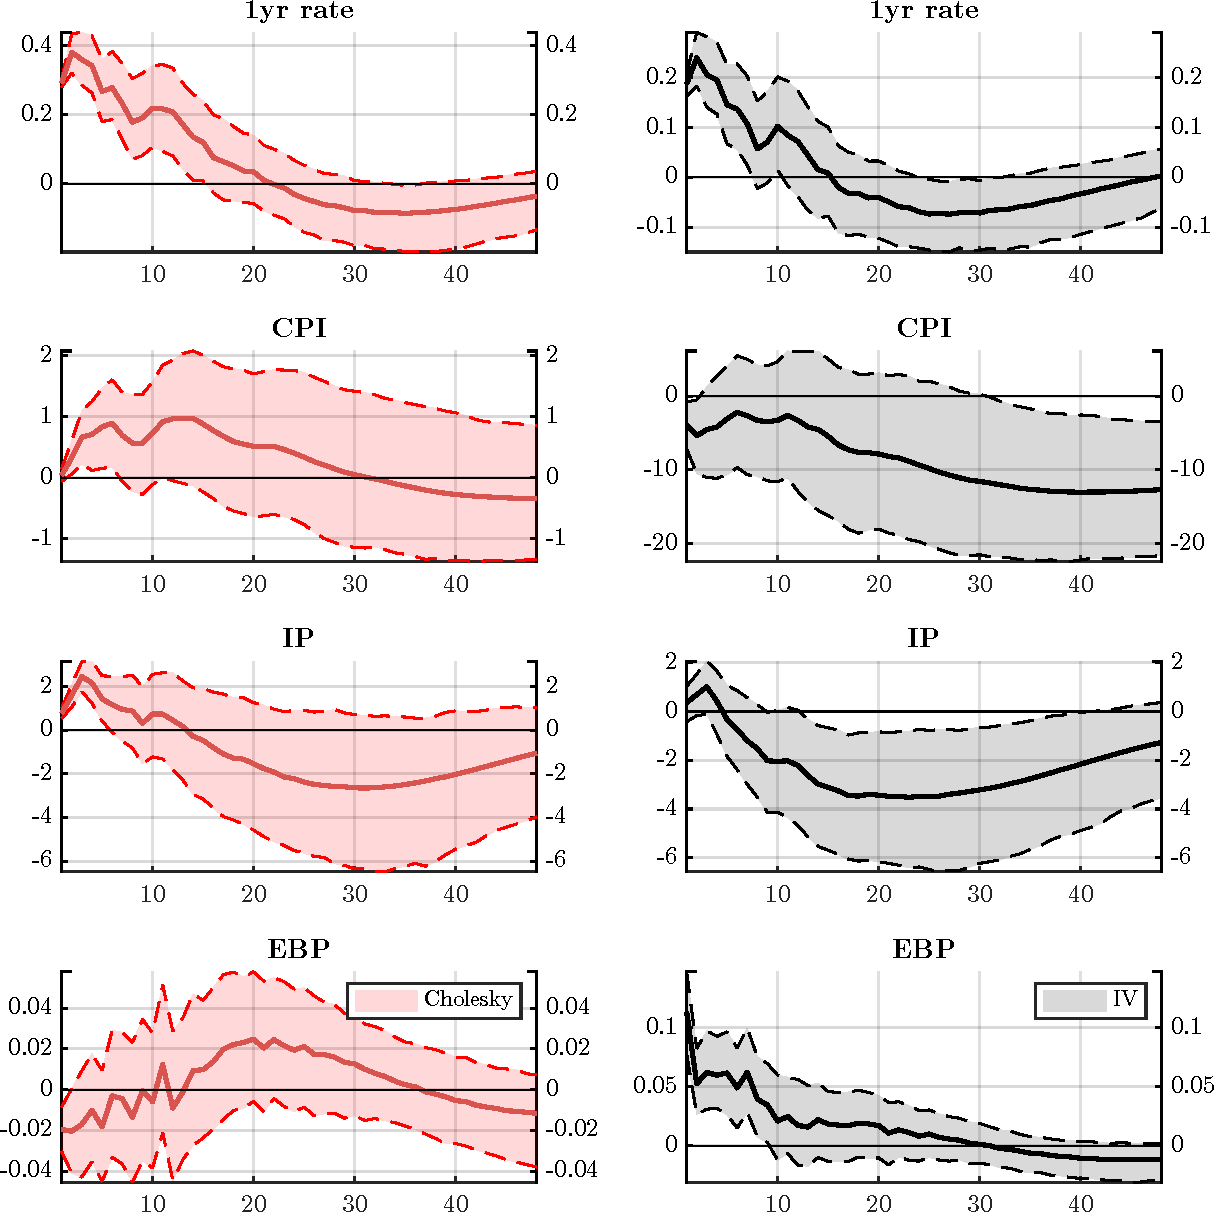
\includegraphics[width=.9\textwidth]{GK_Fig1}
		\end{center}%
		\vspace{0.2cm}
		\caption{\scshape{Gertler and Karadi (2015): Figure~1}}
		\vspace{0.2cm}
		\scriptsize{{\scshape Note.} Impulse responses of the 1-year Treasury bill rate, the consumer price index, industrial production, and the excess bond premium to a contractionary monetary policy shock, comparing two identifications of the same VAR. \textit{Left column (red):} recursive (Cholesky) identification with the policy rate ordered first. \textit{Right column (black):} external-instrument identification (proxy SVAR) using FF4 federal funds futures surprises. Four-variable VAR(12) with constant, estimated on monthly US data, 1979:M7--2012:M6. Horizon: 48 months. Solid line: bootstrap mean. Shaded bands: 95\% wild-bootstrap confidence intervals (500 draws).}
		\label{fig:GK_IR_1}
	\end{minipage}
\end{figure} 

The recursive identification displays the familiar pathologies of timing restrictions in monetary VARs. The price level rises for roughly two years after a contractionary shock --- the \textit{price puzzle} --- and industrial production increases on impact before turning negative, neither of which matches the textbook response to a tightening. The excess bond premium barely moves: its point response hovers near zero and the confidence band straddles zero at every horizon, so the recursive scheme detects no role for credit-spread movements in transmission. 

The external instrument removes these anomalies. The price level now falls and keeps falling over the horizon, industrial production declines to a trough around a two-year horizon, and the one-year rate rises significantly on impact before reverting. Most consequentially for the credit channel, the excess bond premium jumps sharply on impact --- by several basis points --- and the response is statistically significant for the first several months before decaying to zero. The contrast with the muted, insignificant recursive response is the empirical core of \cite{GertlerKaradi2015}: once the policy shock is identified cleanly from high-frequency surprises, a monetary tightening is found to widen credit spreads well beyond the movement in the risk-free rate it induces. This excess-bond-premium response is read as evidence that financial frictions play an important role in the transmission of monetary policy.


%------------------------------------------
\subsection{Jord\`{a} and Taylor (2025): Local Projections and LP-IV}\label{sec:app_jt}

This application illustrates the local projection framework developed in Section~\ref{sec:lp}. In LP-OLS, causal identification rests on the exogeneity of the shock measure $s_t$; in LP-IV, the endogenous treatment $d_t$ is instrumented by an external proxy $z_t$. Both approaches recover impulse responses without fitting a full structural model, but through different identification arguments. \cite{JordaTaylor2025} survey local projections, covering both the case where the shock enters the LP regression directly as the treatment variable (LP-OLS) and the case where the shock instruments an endogenous treatment variable (LP-IV). Their survey also introduces the long-difference specification as a practical device for persistent outcome variables. We replicate their Examples~5 and~6 (Figures~5a and~6a in the paper), which together demonstrate both variants of the LP estimator in the context of monetary policy transmission.

\noindent\textbf{Example~5 (Figure~5a): LP-OLS.}\ The first exercise estimates the response of log CPI (scaled to percent) to a unit Romer-Romer narrative monetary policy shock \citep{RomerRomer2004} using quarterly US data, 1985:Q1--2007:Q4. The Romer-Romer shock $s_t$ is constructed to capture exogenous variation in monetary policy intentions; it enters the LP regression directly as the treatment variable, with no instrumentation required. The dependent variable is specified in long-difference form, $(\log \text{CPI}_{t+h} - \log \text{CPI}_{t-1}) \times 100$. This measures the cumulative change in log CPI from one period before the shock (period $t-1$) to horizon $h$, which is appropriate for persistent series: expressing the outcome as a net change relative to the pre-shock level avoids the level-stationarity problems of a pure level specification. The LP-OLS regression for each $h = 0, 1, \ldots, 18$ is
\begin{equation}\label{eq:lp_ols_jt}
    (\log \text{CPI}_{t+h} - \log \text{CPI}_{t-1}) \times 100 = \alpha_h + \beta_h \, s_t + \gamma_h' w_t + e_{t+h},
\end{equation}
where $w_t$ contains four lags of log real GDP growth, CPI inflation, and the short-term interest rate. The coefficient sequence $\{\hat\beta_h\}_{h=0}^{18}$ directly traces the cumulative CPI response to a unit Romer-Romer shock.

\noindent\textbf{Example~6 (Figure~6a): LP-IV.}\ The second exercise estimates the response of the unemployment rate to a 1 percentage point federal funds rate (FFR) shock using monthly US data, 1985:M1--2000:M1. The FFR is an endogenous variable: the Fed adjusts rates in response to economic conditions, so using it directly as $s_t$ would confound the structural shock with the endogenous policy reaction. The solution is instrumental variables. The Romer-Romer narrative shock $z_t$ \citep{RomerRomer2004}, as used in \citet{JordaTaylor2025}, is a measure of exogenous monetary policy variation constructed from Federal Reserve documents and instruments the FFR. The LP-IV regression for each $h = 0, 1, \ldots, 49$ is
\begin{equation}\label{eq:lp_iv_jt}
    (\text{urate}_{t+h} - \text{urate}_{t-1}) = \alpha_h + \beta_h \, d_t + \gamma_h' w_t + e_{t+h},
\end{equation}
where $d_t$ is the FFR (endogenous treatment) and $w_t$ includes six lags of the unemployment rate, inflation, and the FFR. The instrument set consists of the current Romer-Romer shock and its six lags, $\{z_t, z_{t-1}, \ldots, z_{t-6}\}$. With seven instruments for one endogenous regressor the system is over-identified. The VAR Toolbox estimates the LP-IV horizon by horizon via 2SLS rather than two-step GMM as in \citet{JordaTaylor2025}; this accounts for some of the quantitative differences between the toolbox output and the original paper's results. Under 2SLS with multiple instruments, consistency is maintained but the estimator is not asymptotically efficient relative to two-step GMM. At each horizon, $\hat\beta_h$ recovers the cumulative unemployment response to a unit FFR shock, purged of the endogenous variation in $d_t$.

The conceptual distinction between the two exercises reflects a general principle of the LP framework. In LP-OLS, $s_t$ is a direct, exogenous measure of the structural shock and enters as the treatment: consistency requires that $s_t$ be orthogonal to $e_{t+h}$ (exogeneity) and that $s_t$ retain variation after partialling out the controls $w_t$ (a rank condition). In LP-IV, $z_t$ is a noisy proxy that instruments the endogenous treatment $d_t$: consistency requires both instrument relevance ($\mathbb{E}[d_t z_t'] \neq 0$ after partialling out controls) and exogeneity ($\mathbb{E}[e_{t+h} z_t'] = 0$ for all $h$). The LP-IV estimator applies 2SLS horizon by horizon, without fitting a fully specified dynamic model for the endogenous treatment.

Both exercises use Newey-West standard errors with bandwidth $h - 1$, consistent with the MA($h-1$) structure of the LP residuals discussed in Section~\ref{sec:lp_background}. Confidence bands at 68\% and 95\% are both reported: the narrower 68\% bands are derived from the 95\% bands by rescaling. Under the approximation that the sampling distribution of $\hat\beta_h$ is asymptotically normal, the ratio of standard-normal quantiles $\Phi^{-1}(0.84)/\Phi^{-1}(0.975)\approx 1.00/1.96$ maps the 95\% half-width to the 68\% half-width. Assuming the data have been loaded and samples trimmed to the relevant windows, the key implementation steps are:

\begin{matlabcode}
% LP-OLS -- log CPI response to Romer-Romer shock (quarterly)
LPopt_OLS          = LPoption;
LPopt_OLS.nsteps   = 18;        % 18-quarter horizon
LPopt_OLS.longdiff = 1;         % LHS: lcpi_{t+h} - lcpi_{t-1}
LPopt_OLS.impact   = 1;         % unit shock
LPopt_OLS.pctg     = 95;
CTRL_OLS = [dlrgdp dlcpi dstir];
LP_OLS   = LPmodel(lcpi, rr_shock, CTRL_OLS, 4, 1, LPopt_OLS);
IR_OLS     = LP_OLS.IR;
INF95_OLS  = LP_OLS.INF;
SUP95_OLS  = LP_OLS.SUP;

% LP-IV -- unemployment response to FFR shock (monthly)
LPopt_IV          = LPoption;
LPopt_IV.nsteps   = 49;        % 49-month horizon
LPopt_IV.longdiff = 1;         % LHS: urate_{t+h} - urate_{t-1}
LPopt_IV.impact   = 1;         % unit shock
LPopt_IV.pctg     = 95;
LPopt_IV.IV       = RRCGShock;
LPopt_IV.nlag_iv  = 6;   		   % lags of instrument
CTRL_IV = [urate infl ffr];
LP_IV   = LPmodel(urate, ffr, CTRL_IV, 6, 1, LPopt_IV);
IR_IV     = LP_IV.IR;
INF95_IV  = LP_IV.INF;
SUP95_IV  = LP_IV.SUP;
\end{matlabcode}

Figure~\ref{fig:JT_Replication} reports both exercises side by side: the LP-OLS response in the left panel (the paper's Figure~5a) and the LP-IV response in the right panel (the paper's Figure~6a). The LP-OLS results (Figure~5a) show a negative cumulative response of the price level to a contractionary Romer-Romer shock: log CPI falls by around 2--4 percent (cumulative) over the first 12 quarters, consistent with the standard monetary transmission channel; the magnitude reflects the scale of the Romer-Romer shock measure, which captures large identified policy changes. The LP-IV results (Figure~6a) show that a 1 percentage point contractionary FFR shock raises unemployment, with the response building gradually over 12--24 months before plateauing. Confidence bands are wider in the LP-IV case, reflecting the additional uncertainty from the IV correction and the longer horizon. The comparison between the two exercises illustrates the scope of the LP framework: LP-OLS suffices when a clean shock measure is available, while LP-IV extends the approach to settings where the treatment variable is endogenous and must be instrumented. See Section~\ref{sec:lp} for the general LP framework and its connection to the exogenous-variable SVAR.

\vspace{0.2cm}
\begin{figure}[ht!]
	\centering%
	\begin{minipage}[b]{.9\textwidth}
		\begin{center}
			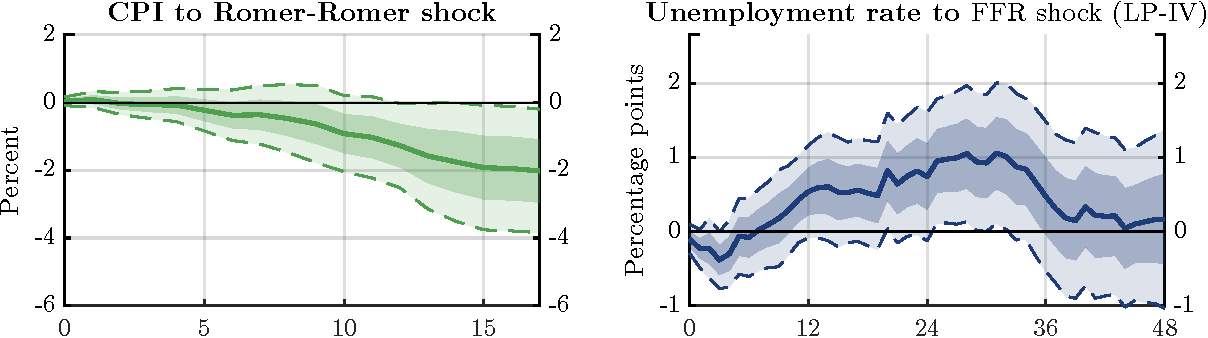
\includegraphics[width=.9\textwidth]{JT_Fig5a_6a}
		\end{center}%
		\vspace{0.2cm}
		\caption{\scshape{Jord\`{a} and Taylor (2025): Figures~5a and~6a}}
		\vspace{0.2cm}
		\scriptsize{{\scshape Note.} \textit{Left (Figure~5a):} LP-OLS impulse response of log CPI ($\times 100$) to a unit Romer-Romer narrative monetary policy shock. Dependent variable in long-difference form: $(\log \text{CPI}_{t+h} - \log \text{CPI}_{t-1}) \times 100$. Controls: 4 lags of log real GDP growth, CPI inflation, and the short-term interest rate. Sample: 1985:Q1--2007:Q4. Horizon: 18 quarters. \textit{Right (Figure~6a):} LP-IV impulse response of the unemployment rate to a 1 percentage point FFR shock, instrumented by the Romer-Romer narrative shock and its 6 lags (2SLS). Dependent variable: $\text{urate}_{t+h} - \text{urate}_{t-1}$. Controls: 6 lags of unemployment, inflation, and the FFR. Sample: 1985:M1--2000:M1. Horizon: 49 months. Shaded bands: 95\% (light) and 68\% (dark) Newey-West confidence bands.}
		\label{fig:JT_Replication}
	\end{minipage}
\end{figure}


\end{document}
  